% arara: xelatex
% arara: xelatex
% arara: xelatex


% options:
% thesis=B bachelor's thesis
% thesis=M master's thesis
% czech thesis in Czech language
% english thesis in English language
% hidelinks remove colour boxes around hyperlinks

\documentclass[thesis=B,english]{FITthesis}[2019/03/21]

\usepackage{todonotes}
\usepackage{graphicx}

\setlength{\fboxsep}{0.005pt}
\newcommand{\tmpframe}[1]{\fbox{#1}}
%\renewcommand{\tmpframe}[1]{#1}


%\usepackage[utf8]{inputenc} % LaTeX source encoded as UTF-8
% \usepackage[latin2]{inputenc} % LaTeX source encoded as ISO-8859-2
% \usepackage[cp1250]{inputenc} % LaTeX source encoded as Windows-1250

% \usepackage{subfig} %subfigures
% \usepackage{amsmath} %advanced maths
% \usepackage{amssymb} %additional math symbols

\usepackage{dirtree} %directory tree visualisation

% % list of acronyms
% \usepackage[acronym,nonumberlist,toc,numberedsection=autolabel]{glossaries}
% \iflanguage{czech}{\renewcommand*{\acronymname}{Seznam pou{\v z}it{\' y}ch zkratek}}{}
% \makeglossaries

% % % % % % % % % % % % % % % % % % % % % % % % % % % % % % 
% EDIT THIS
% % % % % % % % % % % % % % % % % % % % % % % % % % % % % % 

\department{Department of Software Engineering}
\title{Analysis of an IoT solution for assessment of physical difficulty of tourist tracks using smart wearables}
\authorGN{Zuzana} %author's given name/names
\authorFN{Václaviková} %author's surname
\author{Zuzana Václaviková} %author's name without academic degrees
\authorWithDegrees{Zuzana Václaviková} %author's name with academic degrees
\supervisor{Ing. Jan Krákora, PhD.}
\acknowledgements{THANKS (remove entirely in case you do not with to thank anyone)}
\abstractEN{Summarize the contents and contribution of your work in a few sentences in English language.}
\abstractCS{V n{\v e}kolika v{\v e}t{\' a}ch shr{\v n}te obsah a p{\v r}{\' i}nos t{\' e}to pr{\' a}ce v {\v c}esk{\' e}m jazyce.}
\placeForDeclarationOfAuthenticity{Prague}
\keywordsEN{Internet of Things, hiking track difficulty, activity tracking, heart rate monitoring, physical fitness assessment, smart wearables, software analysis, mobile application design, user experience}
\keywordsCS{Internet vecí, náročnosť turistickej trasy, sledovanie fyzickej aktivity, meranie tepu srdca, posudzovanie telesnej kondície, nositeľná elektronika, softvérová analýza, dizajn mobilnej aplikácie, užívateľské skúsenosti}
\declarationOfAuthenticityOption{1} %select as appropriate, according to the desired license (integer 1-6)
% \website{http://site.example/thesis} %optional thesis URL

\graphicspath{ {./Images/} }

\begin{document}

% \newacronym{CVUT}{{\v C}VUT}{{\v C}esk{\' e} vysok{\' e} u{\v c}en{\' i} technick{\' e} v Praze}
% \newacronym{FIT}{FIT}{Fakulta informa{\v c}n{\' i}ch technologi{\' i}}


\setsecnumdepth{part}
\chapter{Task - temporary chapter}
\linebreak
Analysis of an IoT solution for assessment of tourist track physical difficulty

The aim of this thesis is to analyse, design and implement a proof-of-concept \todo{maybe change the way the acronyms are introduced?} (PoC) Internet-of-Things (IoT) solution for tourist track difficulty estimation.
Using a mobile application, the user shall be able to select a track and assess how difficult the specific part of the track will be for them, based on data collected from similarly fit users.
\begin{itemize}
    \item Analyse and compare similar existing solutions.
    \item Analyse and design an IoT solution for data processing.
    \item Design a mobile application for data visualization and track selection.
    \item Create a PoC of the IoT platform and of the mobile application.
    \item Collect raw data from smart watch heart rate sensors and smart phone GPS locators and propose relevant statistics to process this data.
\end{itemize}


\setsecnumdepth{all}
\chapter{Introduction}
With the increasing popularity of smart wearables in the general public, a growing number of people have been able to benefit from adjustments in their behaviour according to the way their data gets processed and fed back to them.
Runners can barely imagine not checking how fast and how efficiently they just ran their daily track or how much they have improved over the last month,
people with sedentary jobs attempt to keep their daily step count above a currently recommended number,
masses of people have been saving up for the Apple Watch 5~\cite{AppleWatch5} in spite of the ECG health monitor being virtually unnecessary for those not at risk of cardiac disease~\cite{ecg-screening}, etc.

All of this data is collected from a variety of devices, such as smartwatches, textiles with integrated sensors, jewelry, or more invasive ones such as implants or tattoos, all of which are meant to be worn on the user's body and which measure and send data for analysis - hence the name \textit{wearable technology}, or \textit{smartwear}~\cite{what-is-wearable-tech}.

Thanks to the data collected from these devices, the users have been keeping track of their health and fitness, setting goals for themselves and tracking personal achievements.
However, all of this is related to the past of each individual user, while the true potential of smartwear lies in collecting data from thousands of people,
finding patterns and correlations in large datasets and using the results to increase precision and improve upon whatever the data is being used for by the virtue of prediction.

That being said, the result of this thesis will be a design for an IoT solution, mainly to be used by hikers who want to not only pick a track on a map and see how long it is going to take them to get from point A to point B (which generally isn't tailored to the individual's fitness and often doesn't account for the possible rapid changes in the track's elevation profile),
but also an objective difficulty level of particular sections of said track, which may have additional benefits for people with cardiac issues or those trying to lose weight, who are interested in some more detailed insight into the exertion induced by the track in order to keep their heart rate in a specific range.
All of this will be available to the user before stepping foot on said track, thanks to the data collected from users with various fitness levels and their own history,
while the user's fitness will be presented more accurately as they continue to use the application.

I will study how fitness is assessed in regard to feasibility, availability for the general public, and precision, in order to provide fundamentals for further work.

Using methods of software engineering, I am going to analyse the use of wearable technology in existing applications and document the most common features as well as their outstanding traits and their use of IoT principles (or lack thereof).
Based on this analysis, I will pick the most relevant features to include in my design and extend them with features of my own devising, which will set my solution apart from existing software.

I will design and implement a PoC IoT solution -- a mobile application which will collect data from the smartwear sensor and an available GPS locator, along with a backend IoT platform to receive and process collected data, and the communication channels used between these two modules.
I will neither design nor implement a full-fledged IoT platform as that's not in the scope of this thesis.
I will design (not implement) the frontend mobile application for displaying of processed data, track selection with integrated maps and explore the necessary legal requirements for the use of such maps.

I will examine the use of different device types with heart rate sensors and choose one with which I will build my PoC.

I will collect and perform suitable operations on the collected data in order to visualize it.


\chapter{Aims}
The aim of this thesis is to analyse and design the functionality \todo{reword} of an IoT solution for assessment of tourist track difficulty, based on the individual's fitness.

In the theoretical chapters I will analyse existing applications in the domain of fitness trackers and e-health, assess the importance of specific features to the application's main usecases
and apply the results of this research to my own approach when determining the requirements for the system.
Based on these requirements, I will design the front-end of a mobile application for track selection and data visualization.
I will also design the overall architecture of the PoC solution.

In the practical part of the thesis I will focus on implementing a PoC of the designed solution - a mobile phone application for data collection and a platform for data receiving, with emphasis on usage of relevant data science methods. \todo{reword}

\chapter{Fitness assessment}
Since the platform should estimate how a user will be affected by a hike, there needs to be some way of assessing their fitness to make the estimates legitimate instead of just guessing.
This is why this chapter studies modern methods of fitness testing, the variables that need to be considered, and the accuracy and feasibility of such tests.

A physical fitness test usually evaluates multiple components of one's health, including cardiovascular endurance, muscular strength, muscular endurance, flexibility and body composition.

I will focus on familiarizing the reader with cardiovascular endurance testing since the heart, lungs and blood vessels are what gets exerted the most during hiking.
There are other indicators that one can measure (such as the lactate threshold - a non-linear increase in blood lactate concentration~\cite{lactate-threshold}), 
but the most popular and easiest to measure with affordable sensors is VO2 max.

\section{VO2 and VO2 max}

The volume of consumed oxygen (VO2) is closely correlated with heart rate, respiration rate, and on/off-dynamics, all of which can be derived from RR interval data (time elapsed between two successive R waves -- the tallest spikes on an ECG),
with respiration rate being able to differentiate between metabolic (physical activity-induced) and non-metabolic (mental and non-exercise related physical stress) changes in heart rate,
which makes models that take it into account highly accurate compared to those which only use heart rate~\cite{vo2-hr-firstbeat}.

VO2 max, the maximal value of VO2, is considered the most accurate metric of cardiovascular fitness.

Measured in millilitres of oxygen consumed per minute or millilitres of oxygen per kilogram of bodyweight per minute, it is the amount of oxygen the body is able to effectively use (transform to energy) during intense or maximal exercise.
With the growing amount of oxygen the body can consume, it can perform better during strenuous activity and give improved results~\cite{vo2max-definition}.
This is limited by the ability of the cardiorespiratory system to deliver oxygen to the exercising muscle, thus making it impossible for an athlete to operate above 100\% of their VO2 max for extended periods~\cite{vo2max-oxygen-delivery}.

\begin{figure}[h]
    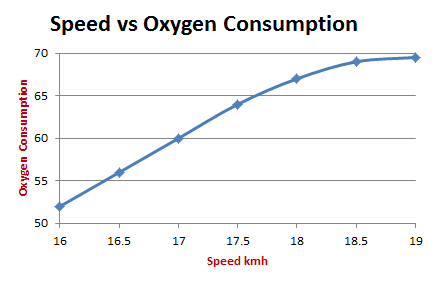
\includegraphics[width=\textwidth]{V02max-running.png}
    \caption{With increasing speed of the runner, oxygen consumption increases linearly and plateaus around 18.5 kilometres per hour - the VO2 max~\cite{vo2max-speed-img}.}
\end{figure}

\subsection*{How to measure Vo2 max}

\subsubsection*{Laboratory test}

Typically, VO2 max is measured directly in laboratory conditions while wearing a respiratory mask, by analyzing inspired and expired breathing gases during maximal exertion~\cite{vo2max-definition}, usually running on a treadmill or riding a stationary bike.

This method of determining VO2 max is highly accurate, but given the need for expensive equipment and trained staff, laboratory testing just isn't feasible for everyday population-wide testing.
On the other hand, results from laboratory tests are often used as reference values for determining the accuracy of alternative methods.

\subsubsection*{Cooper test - Twelve-Minute Run-Walk}

First suggested in the 1970's, Cooper's Twelve-Minute Run-Walk is an endurance test, where the main goal is to run (or walk) as long a distance as possible in twelve minutes.
It was originally developed mainly for armies and police agencies, but it's also popularly (and unnecessarily~\cite{cooper-pupils}) used in schools on untrained pupils.
It is inaccurate for people who do not train running and swim or bike instead, as their bodies are used to a completely different set of movements.

There is a high correlation between the distance an individual can run and their VO2 max value, which can be calculated thusly:

$VO2max = (22.351 \times distance\_in\_kilometers) - 11.288$~\cite{cooper-vo2max}.

\subsubsection*{Multistage Fitness Test - Beep test}

Introduced by a Canadian sports scientist Luc Léger in the 1970s, this aerobic test has consistently been found a reliable way of finding a person's VO2 max.

The original version of the beep test (the Track Test) had the participants running back and forth in the interval of two minutes while the running pace was increased, so they always had to run further than in the previous iteration.

This test was highly efficient, however, given the long intervals and spatial requirements, it couldn't be performed indoors, giving rise to modifications, such as the Twenty-Metre Shuttle Run Test.
As the name suggests, two markers are placed twenty metres apart and again, the participants run back and forth between them, trying to reach the opposite marker before the next -- shorter -- stage begins, that is, before the next beep.
Once the test subject fails to reach a marker, turns without touching the marked line, or starts running before the signal, after one warning, their test is over.
They can also choose to stop when they have reached their maximum physical limit.

The test is divided into stages with recommended running speeds, each stage consisting of multiple shuttles - see the table at~\cite{beep-test-scoring-table}.
From the stage and shuttle reached, one can calculate the VO2 max using the formula

\[VO2max (\frac{ml}{kg*min-1}) = 31.025 + 3.238X - 3.248A + 0.1536AX\]

where $A$ is age of the participant and $X$ is the speed in the final shuttle.
This formula fits the commonly used version of the Beep test (starting at 8.0 km/h, jumping to 9.0 km/h and continuing to rise by 0.5 km/h per level) and may vary depending on the version used~\cite{beep-test-versions}~\cite{beep-test-20m-valid}.

This modified version (just like the original) has been recognized as a valid method to determine VO2 max of male and female adults, individually or in groups, on most gymnasium surfaces~\cite{beep-test-20m-valid}.

In 2017, Tomkinson et al. published a complex systematic study of nearly 1.2 million 9-17 years old children from 50 countries with data from beep tests as old as 1981,
setting standardized norms for testing of fitness in the world's youth~\cite{beep-test-youth-large-study}.


\subsubsection*{Six-Minute Walk Test}

There are also some non-running tests which can be used to measure an individual's VO2 max.

The Six-Minute Walk Test, or 6MWT for short, originated from the Cooper test in the 1980's as a more feasible and less exhausting alternative~\cite{6mwt-history}.

The main objective is for the participant to walk as long a distance as they can in the provided six minutes on a 15- or 30-metre long track, making sharp turns at the end.
Mänttäri et al. published a study in 2018~\cite{6min-walk-test-mantarri}, aimed to develop a prediction model for VO2 max based on 6MWT results combined with heart rate at the end of the 6MWT and easy-to-measure anthropometric and demographic data (such as weight, height, age and gender).
The different track lengths only showed negligible differences between distances walked (on average, 23.5 m longer on the 30-m course).
\textit{For men, the best predictors for VO2max were walking distance, age, BMI, heart rate at the end of 6MWT and height, and for women, walking distance, age and weight} -- surprisingly, heart rate wasn't a significant factor for the female participants.

The formula they developed for men:

 $VO2 max=110.546 + 0.062\times distance - 0.25\times age - 0.486\times BMI - 0.42\times height - 0.109\times HR$

 and for women:

 $VO2 max=22.506 - 0.271\times weight + 0.051\times distance - 0.065\times age$

 \textit{where $weight$ is body weight (kg), $distance$ is distance walked in 6 min (m), $age$ (years), $BMI$ is calculated body mass index (kg/m2), $height$ is body height (cm) and $HR$ is heart rate at the end of the walking test (bpm).}

The authors themselves conclude that their output should be cross-validated with new independent samples of the adult population,
but they consider it a precise enough method to be used for public health monitoring in adults.

Another study from 2015~\cite{6min-walk-test-burr} instead used resting heart rate and arrived at this formula:

$VO2 max =70.161 + 0.023 \times distance - 0.276 \times weight - 6.79 \times sex - 0.193 \times resting_HR - 0.191 \times age$

using $distance$ walked during 6MWT (m), $weight$ (kg), $sex$ -- 1 for female, 0 for male, and $resting_HR$ for resting heart rate in beats per minute.

\subsubsection*{Sit-to-Stand test}

Another test that doesn't require much in terms of space or equipment and is in fact a common daily activity, which is often used to test lower body strength and endurance in older adults, has been studied for correlation with VO2 max values.
The Sit-to-Stand test, which consists of repetitive sitting down and standing up, has acquired a number of different forms just like most other tests used by the general public.
The versions include but aren't limited to the incremental twelve-minute STS test -- sit and stand in incrementally shorter periods of time, repeated for twelve minutes, often controlled by a metronome~\cite{seat-height-sit-to-stand};

Having been closely studied by Nakamura et al., it is a potentially valid test (when done with arm support, to increase the complete exhaustion threshold, and the right chair height, among other factors), but more research needs to be carried out to find a suitable version~\cite{frequencies-sit-to-stand}~\cite{validity-sit-to-stand}.

\subsubsection*{Non-exercise tests}

There are also some tests that do not require exercise and instead, have the individual fill out a questionnaire, such as the Jackson test~\cite{nonexercise-vo2max-test-jackson} or the George test~\cite{nonexercise-vo2max-test-george},
which ask questions on the topic of an individual's exercise habits, such as their perceived level of activity over the last six months.
Every answer has a specific weight in the resulting equation, based on which the person's fitness is evaluated.

These tests, however, should not be used as a sole source of information especially in medicine, as the data is self-reported and may be influenced by bias or conscious falsehood.

\section{The Performance Condition}

A person's VO2 max is recognized as their baseline fitness level index, however, everybody has days when they perform better, and days when they perform worse, while the factors in play are the amount of sleep they get, being sore from previous workouts, and general physical and mental wellbeing.

That is why Firstbeat introduced the Performance Condition.

Firstbeat is a provider of physiological analytics for sports and well-being who have translated human physiology into mathematical models based on heart rate variability (see below).
They provide their analytics engine as a service to a number of fitness device manufacturers, such as Garmin, Xiaomi, Honor and others.

The Performance Condition is a real-time index of a user's immediate fitness and fatigue level compared to their baseline fitness level.

This indicator is measured on a scale of -20 to +20, with each point representing roughly 1\% of their Vo2 max.
So if the user's current Performance Condition is +4, they can expect to perform outstandingly,
but at the same time, during the course of a workout, this number will decrease as fatigue from the exercise gets closer~\cite{performance-condition-firstbeat}~\cite{performance-condition-garmin}.

According to Firstbeat's support personnel, the formula behind the Performance Condition is protected information,
but generally, it uses a combination of personal background data, internal and external workload data, and special guidance from the Firstbeat analytics engine~\cite{firstbeat-performance-condition-emails}.
Garmin's support website provides similar information: it is calculated based on the user's pace, heart rate and heart rate variability (HRV)~\cite{performance-condition-garmin}.

HRV is the variability in intervals between cardiac cycles.
It can be demonstrated, for example, by feeling one's pulse on the wrist while resting and breathing deeply - the interval shortens (heart beating faster) when breathing in, and lengthens (heart beating slower) when breathing out~\cite{hrv}.
It's a complicated enough metric that to calculate it accurately, HRV should be measured using a chest strap,
an intrusive heart rate monitoring method which generally isn't available to a runner on a daily basis.

Additionally, the only activities that are currently supported for determining the Performance Condition, are running and cycling,
and the methods Firstbeat has developed to measure it has failed to satisfy a number of users, leading to them not paying much attention to the metric or outright ignoring the values~\cite{performance-condition-unreliable1}~\cite{performance-condition-unreliable-reasoning}.
One of the reasons behind their dissatisfaction is the fact that the metric only connects the effort the user is making with the distance they are covering,
without taking into account the steepness of the slope, the humidity, temperature, and other external factors 
and should be perceived more as an indicator of simply how much effort your body is making (as explained in BHerman's comment on a post~\cite{performance-condition-unreliable-reasoning} in Firstbeat's forum), 
while being marketed as a highly precise metric that shows you how your training is going and not really explained well to the users.

\section{Heart rate zones}

Everybody has a resting heart rate (for example, right after waking up from a good night's sleep), and a maximum heart rate (the highest number of beats per minute achievable).
The range between HR min and HR max is commonly divided into five zones, based on the effort necessary and the effects the heart rate induces in a person:
\begin{itemize}
    \item Zone 1 (Warm-up and very light exercise) --
    The trainee is relaxed at an easy pace and breathes rhythmically. Keeping one's heart rate in this zone helps with recovery from previous activities.
    \item Zone 2 (Easy, light exercise) --
    The trainee exercises at a comfortable pace, is able to hold a conversation and breathes slightly deeper. This zone is good for endurance practice.
    \item Zone 3 (Aerobic, moderate exercise) --
    At a moderate pace, it is more difficult to hold a conversation. Training in this zone helps improve aerobic capacity.
    \item Zone 4 (Threshold, hard exercise) --
    Training at a fast pace is somewhat uncomfortable, the trainee breathes forcefully. This zone is good for improving speed.
    \item Zone 5 (Maximum) --
    The trainee is at a sprinting pace, which is unsustainable for long period of time, and their breathing is laboured.
    This zone helps increase power in the trainee's body~\cite{garmin-heart-zones}~\cite{polar-heart-zones}.
\end{itemize}

Calculating HR min is an easy enough task - just measure your heart rate right after enjoying some good sleep; HR max is trickier.

\subsection*{Running methods to calculate HR max}
There are some methods to get HR max by running, such as running towards a hill at a high intensity and then ascending the hill at as high intensity as possible,
or, on flat ground, running 400 metres at high intensity and then increasing the intensity for another 400 metres.
These tests are considered stress tests, and individuals who are not highly active are not advised to take them~\cite{hrmax-running-tests}.
Another method is based on interval running:
two intervals, four minutes each, in which the trainee is short of breath, interspersed by three minutes of active rest, and finished by a third interval, where two minutes in the trainee increases their speed as much as they can and run for as long as they can.
HR max is the maximum heart rate achieved~\cite{hrmax-running-tests-intervals}.

\subsection*{Age-based methods to calculate HR max}
As the running methods are generally too difficult to do `on the spot', there have been attempts to calculate HR max based on readily available data.

The most commonly used formula to get one's maximal heart rate,\linebreak $HRmax=220-age$ also known as the Fox formula, has been time and time again found largely inaccurate.
Originally intended as a rough formulation, with cross-sectional data from participants who are by no means representatives of a population~\cite{220-hrmax-new-formula} and based on unoriginal research~\cite{220-hrmax-disproved},
a number of researchers have tried to find similarly simple but more accurate formulas, most of them claiming to have found the right one.
One of the popularly used is the cross-sectional research of Tanaka et al., who formulated the equation $208-0.7\times age$.
This formula was later validated by Gellish et al. in 2007 by conducting an analysis of longitudinal data from participants from various groups and developing a similar formula $207-0.7\times age$,
however, both Fox and Tanaka were disproved by Sarzynski et al. in 2014 as not precise enough based on standard error of estimate (12.4 and 11.4 bpm respectively) of the two formulas~\cite{hrmax-age-disproved}.
In that study, Sarzynski stresses \textit{the importance of finding and validating other measures to be used in exercise prescriptions for the determination of intensity of exercise, the estimation of fitness levels, and as a criterion for achieving maximal exertion.}

The HUNT fitness study carried out on over three thousand people by Nes et al. found a more accurate formula $211-0.64\times age$, with the standard error of estimate of 10.8 bpm, but couldn't find evidence of interaction with gender, physical activity, VO2 max or BMI~\cite{hrmax-Nes-HUNT}.


It seems that computational models for peoples' fitness leave a lot to be desired,
but this can all be remedied with further research.

\chapter{Existing solutions}
There's a plethora of applications taking advantage of wearable tech, not all of them using the available bio sensors, ranging from basic real-time heart rate monitoring to progress tracking, to calorie measuring, and to social network sized fitness communities.

In this chapter I will research a few such applications, compare and rate them based on following criteria. \todo{add weight to individual points}
\begin{itemize}
    \item Use of IoT possibilities -- use of available sensors, data collection from the community,
    \item User fitness assessment -- how the user's fitness is assessed (attempt self-assessment, fill out a questionnaire, or take a physical test),
    \item Track difficulty assessment -- how the track's difficulty is assessed (user-reported, or calculated)
    \item Community -- built-in sharing options, possibility for interaction between users,
    \item Extra features -- interesting perks outside of the scope of my app,
    \item User-friendliness -- navigation around the mobile application - finding the general settings, creating and clearing a route, general user experience,
    \item Availability -- is the application or its parts free, paid or are there microtransactions,
    \item Cross-platform -- major operating systems supporting the mobile application and sensors, if any are used,
    \item Propriety -- whether the solution is open-source, closed-source or else.
\end{itemize}


\subsection{komoot}
The cross-platform application for outdoor track suggestion can also be used as a tour planner, a map and a navigation system.

\todo[color = green]{add numeric ratings}

\subsubsection*{Use of IoT possibilities}
Given its use of GPS sensors, komoot does qualify as a basic IoT system, however, it also relies heavily on user input for track rating.
The smart watch only gets used for displaying of routes and navigation, not taking any advantage of the available sensors.
\subsubsection*{User fitness assessment}
When a user is creating a route, they can set its difficulty as one of five levels, 
describing the user's self-reported physical fitness and their current taste for a challenge (or lack thereof): Couch Potato, Average, In Good Shape, Athletic, and Pro.
This parameter is considered when the app is generating a suitable route -- presumably by trying to adjust the elevation profile of the possible routes.
The user's real fitness is not taken into account.
\subsubsection*{Track difficulty assessment} 
Thanks to the maps provided by the OpenStreetMap, users are able to pick a starting point, a destination, as well as any number of waypoints in between for their route.
Once the route is chosen, the user can go through the route's stats - the estimated time it will take to get from start to finish, its length, the elevation profile (uphill, downhill, highest and lowest points, estimated average speed) and the surfaces and their use in proportion to the route's length.
All this information is delivered in easy-to-understand charts as well as interactive mappings -- using a slider, the user can see which stat applies in which part of the route.

\begin{figure}[h]
    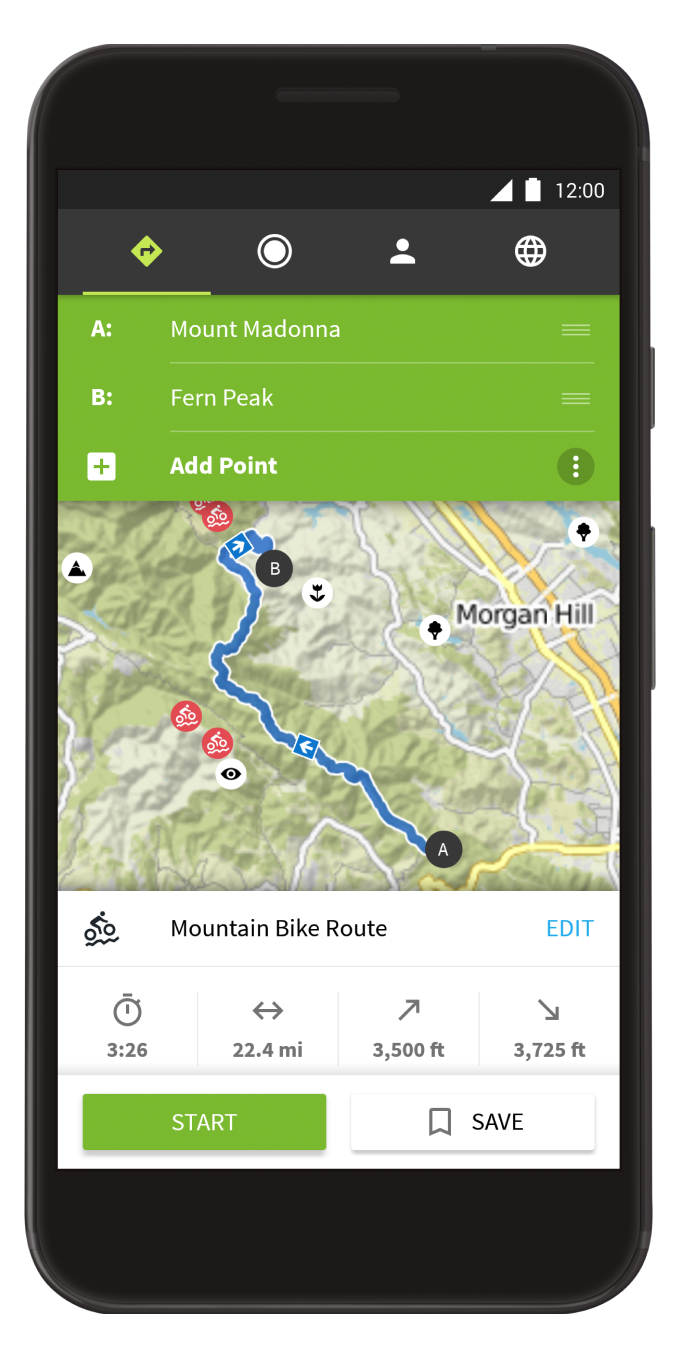
\includegraphics[width=\textwidth]{komoot-nav.png}
    \caption{Offline maps in the komoot app\cite{komoot-nav-img}}
\end{figure}

\begin{figure}[h]
    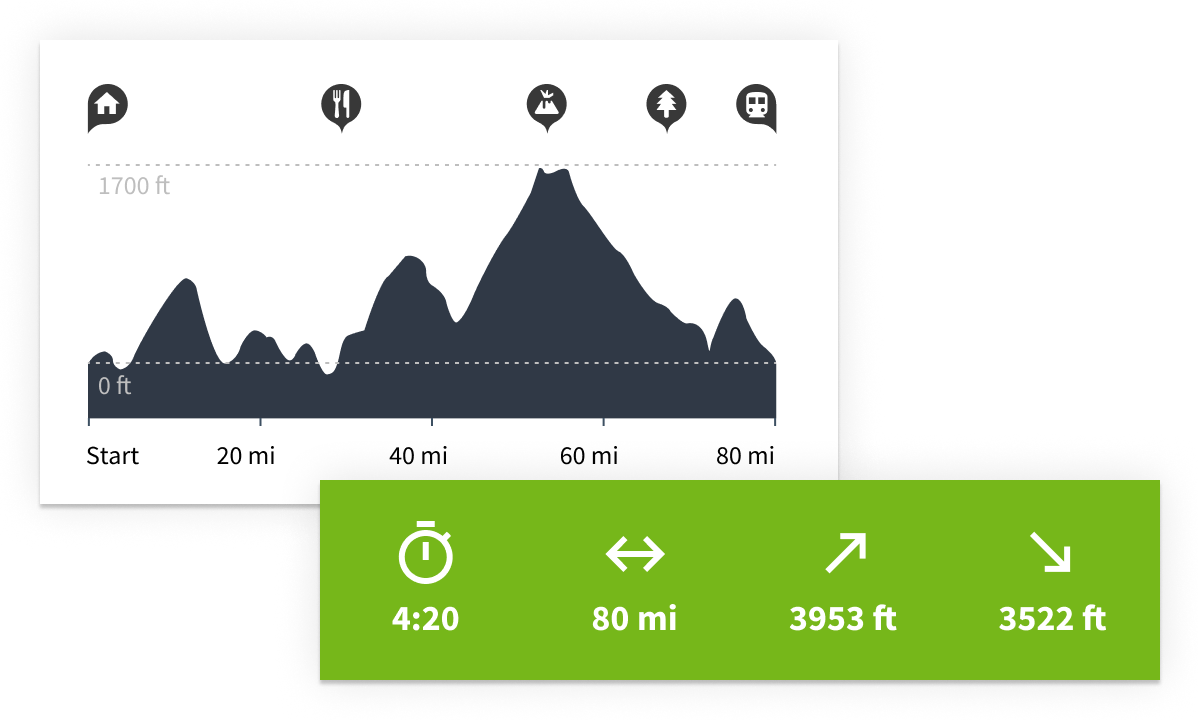
\includegraphics[width=\textwidth]{komoot-route-details.png}
    \caption{Route elevation profile\cite{komoot-route-details-img}}
\end{figure}

\begin{figure}[h]
    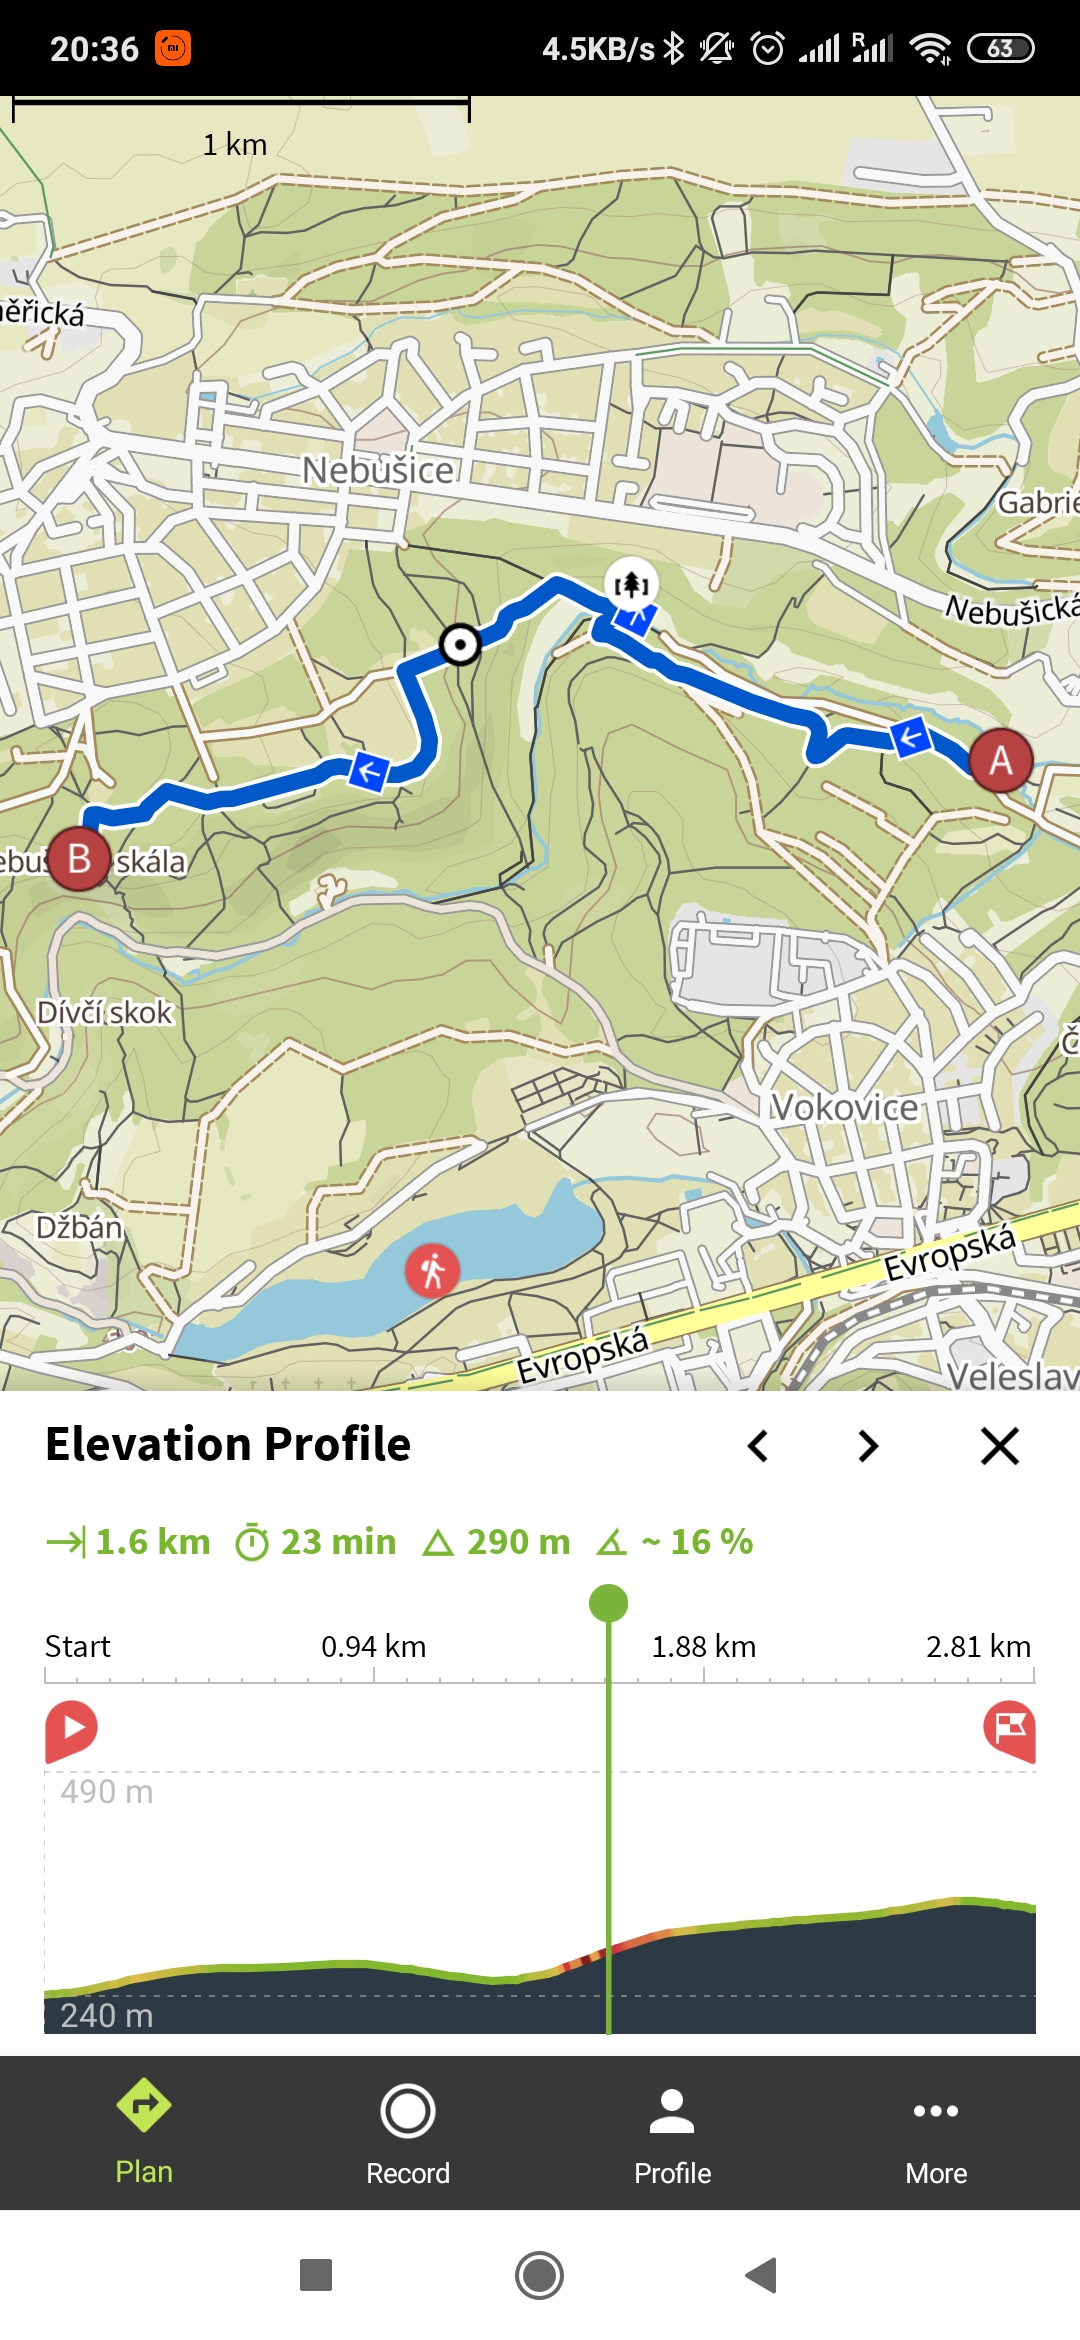
\includegraphics[width=\textwidth]{komoot-route-elevation-detail.jpg}
    \caption{Detailed view of the route's elevation\cite{komoot-route-elevation-detail-img}}
\end{figure}

\begin{figure}[h]
    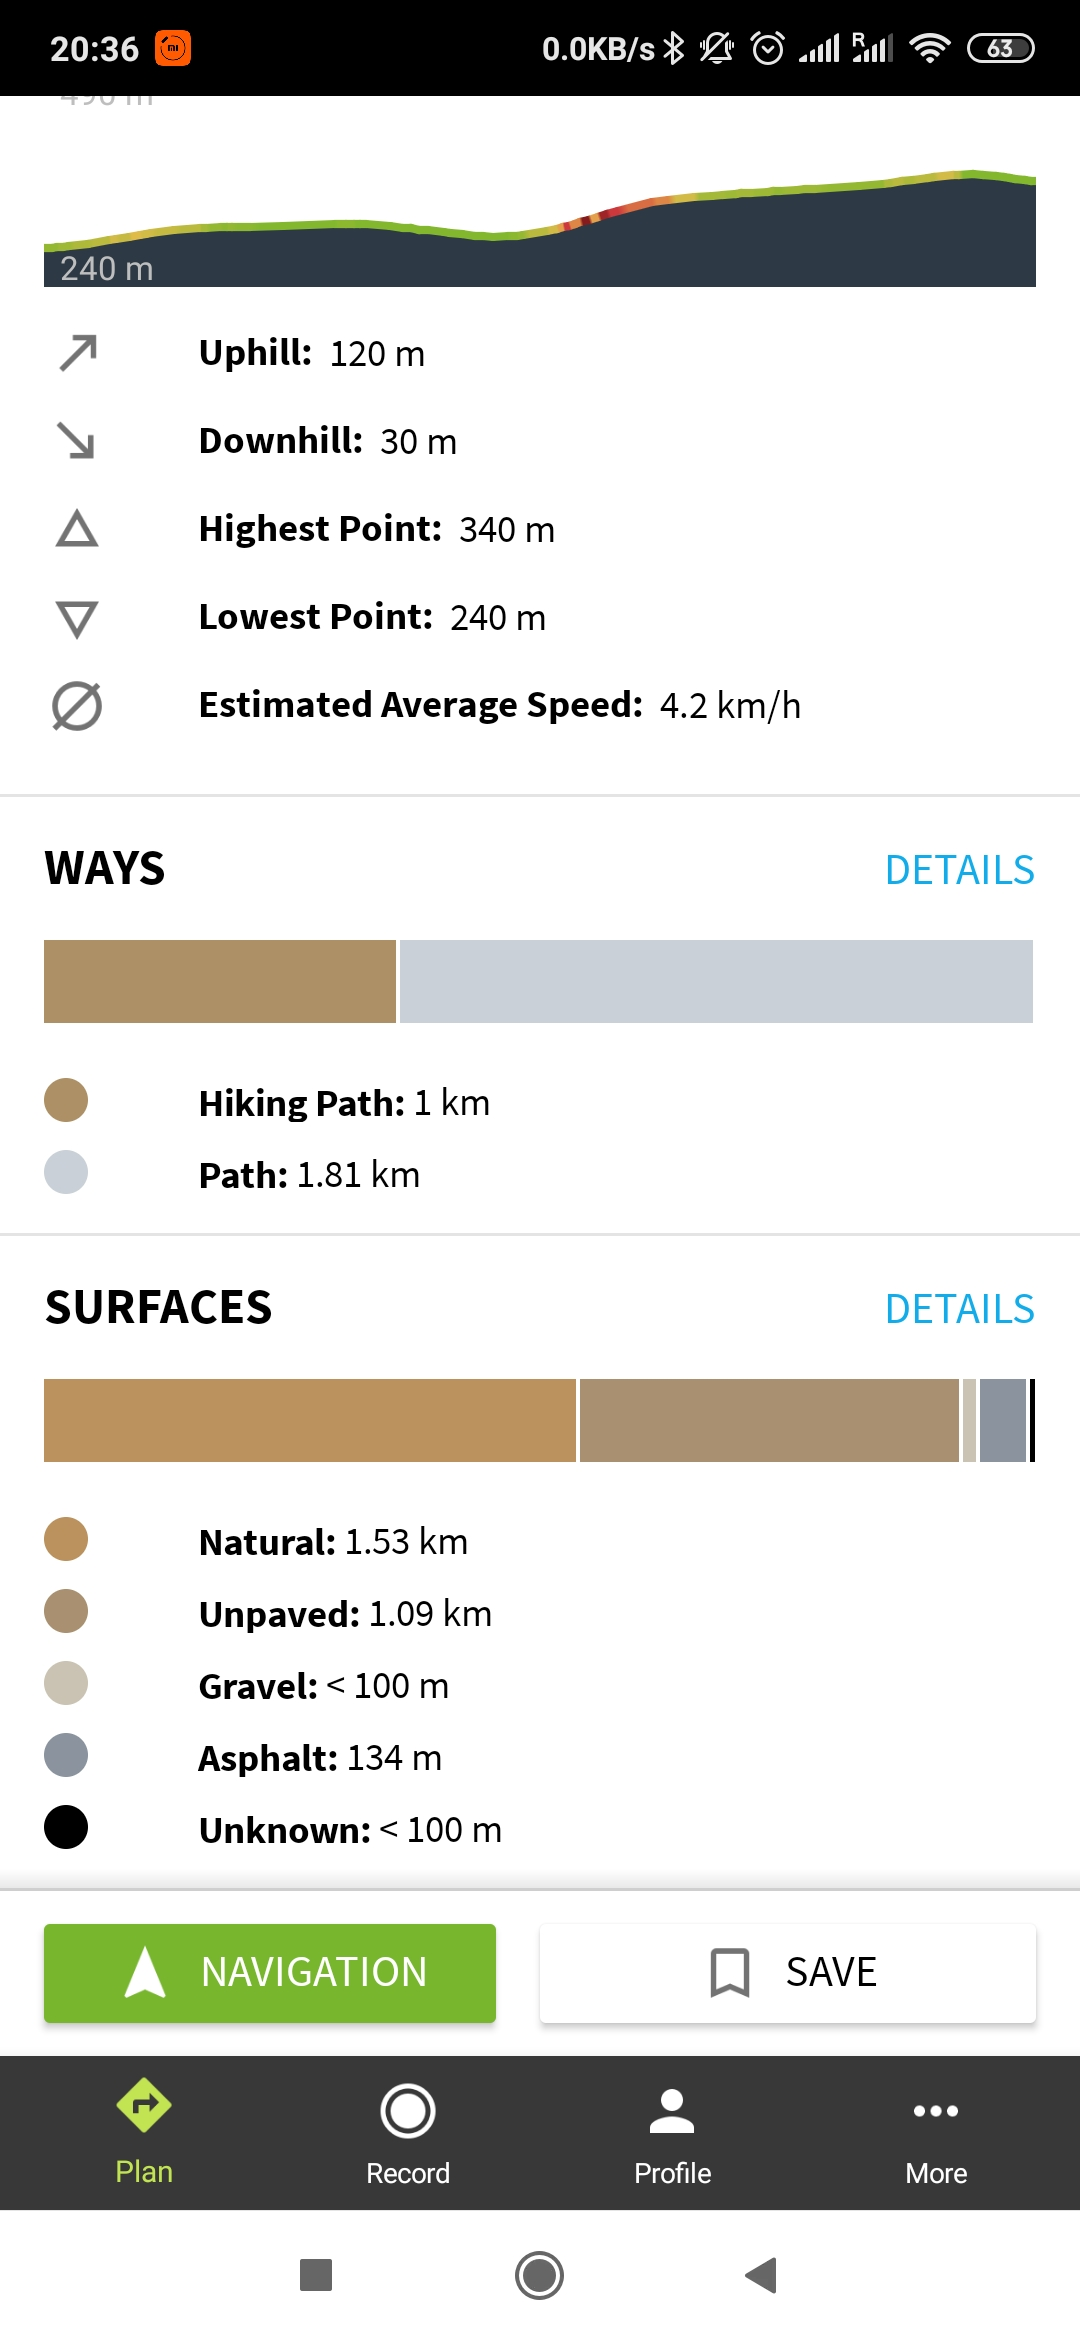
\includegraphics[width=\textwidth]{komoot-route-surface-detail.jpg}
    \caption{Overview of the route's surface. The detailed view is similar to the elevation detail.\cite{komoot-route-surface-overview-img}}
\end{figure}


\subsubsection*{Availability}
The region-based pricing model allows users who do not travel too much to use the app for free,
since the first region is provided at no cost.
In the other pricing options Single Region, Region Bundle and All Regions -- the price-performance ratio seems to grow at a reasonable scale.\todo[color = green]{anything to add?}
\subsubsection*{Community}
With features like sharing of routes users have taken, following of other users, upvoting and commenting on their posts, the mobile application integrates a full-fledged social network.
\subsubsection*{Extra features}

\subsubsection*{User-friendliness}
The navigation through the mobile app takes some time to get used to -- it took me a while to find the Settings after I didn't see them in the burger menu on the bottom navigation bar, which contained only the different pricing options.
Once I created a route, the information provided was well-delivered and easy to read, however, there was no obvious way of completely cancelling the chosen route and picking another one.
Instead, hiding in the Options of the route -- which at first I didn't even notice -- I found the "Reset route" option, which did just what I needed.
Overall, the app has some great parts and some not-so-great ones.
\subsubsection*{Cross-platform}
The system is fully integrated with the Apple Watch and Samsung gear, and -- at least limitedly -- supports a number of other brands of smart watches and other Bluetooth-enabled devices.
The mobile application runs both on iPhones and Android phones.
\subsubsection*{Propriety}
The system is not entirely open-source, as a few of their repositories are public, but the core components remain proprietary. \todo[color = green]{recheck}\todo[color = green]{cite https://github.com/komoot}

\subsubsection*{Overall evaluation}
While being rich with features, komoot doesn't base its functionality on objective data -- it's the users themselves who rate and recommend the specific routes,
an approach in its nature prone to error and with only limited ways of eliminating the human factor.

\subsection{endomondo}
https://www.endomondo.com/
\subsubsection*{Use of IoT possibilities} --
\subsubsection*{User fitness assessment} --
\subsubsection*{Availability} --
\subsubsection*{Community} -- 
\subsubsection*{Extra features} -- 
\subsubsection*{User-friendliness} -- 
\begin{figure}[h]
    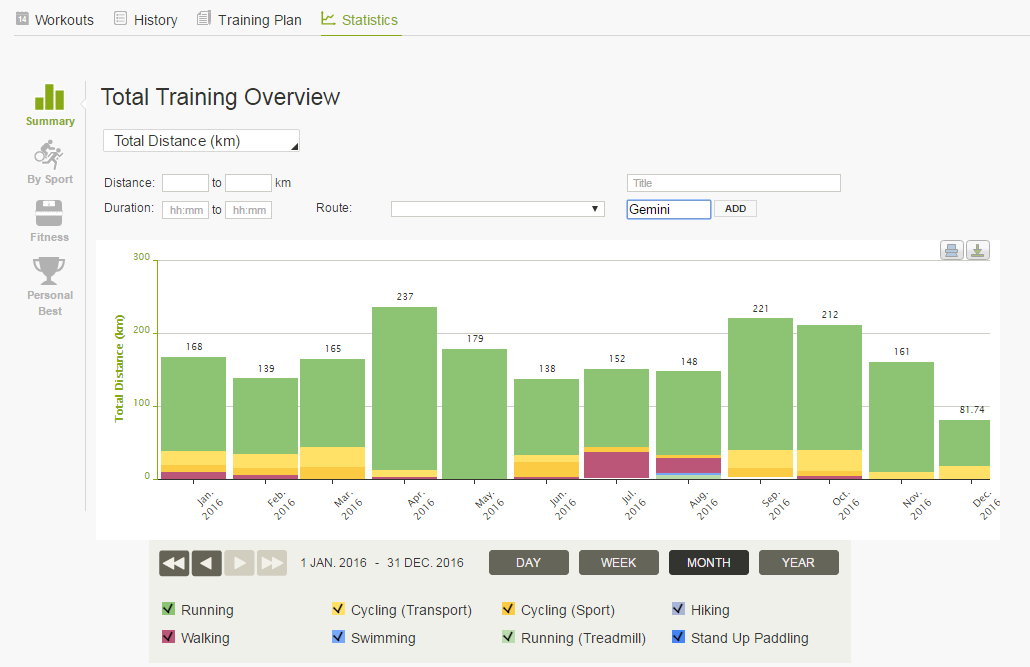
\includegraphics[width=\textwidth]{endomondo-history-example.png}
    \caption{endomondo history example\cite{endomondo-history-img}}
\end{figure}

\begin{figure}[h]
    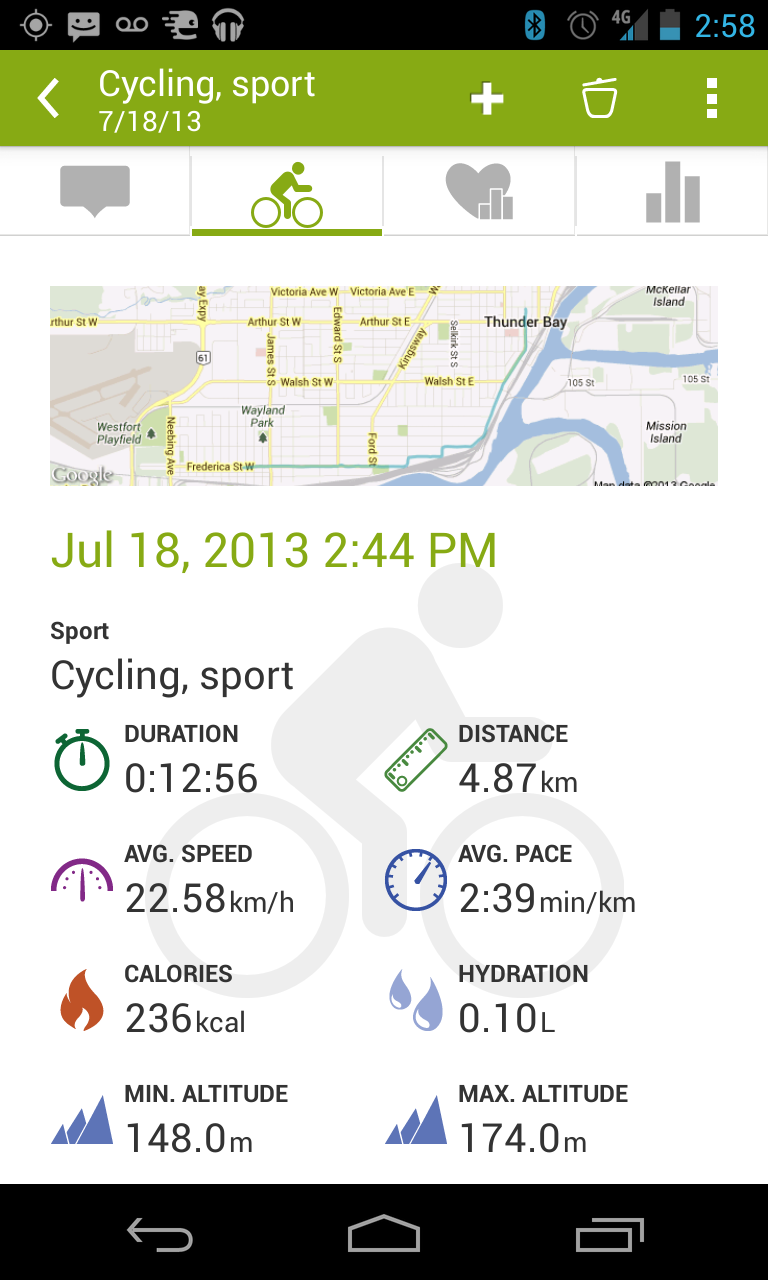
\includegraphics[width=\textwidth]{endomondo-bike-stats.png}
    \caption{Statistics of a biking trip on endomondo\cite{endomondo-bike-stats-img}}
\end{figure}

\subsubsection*{Cross-platform} -- 
\subsubsection*{Propriety} -- 
\subsubsection*{Overall evaluation}

\subsection{Strava}
https://www.strava.com/
\subsubsection*{Use of IoT possibilities} --
\subsubsection*{User fitness assessment} --
\subsubsection*{Availability} --
\subsubsection*{Community} -- 
\subsubsection*{Extra features} -- 
\subsubsection*{User-friendliness}
\begin{figure}[h]
    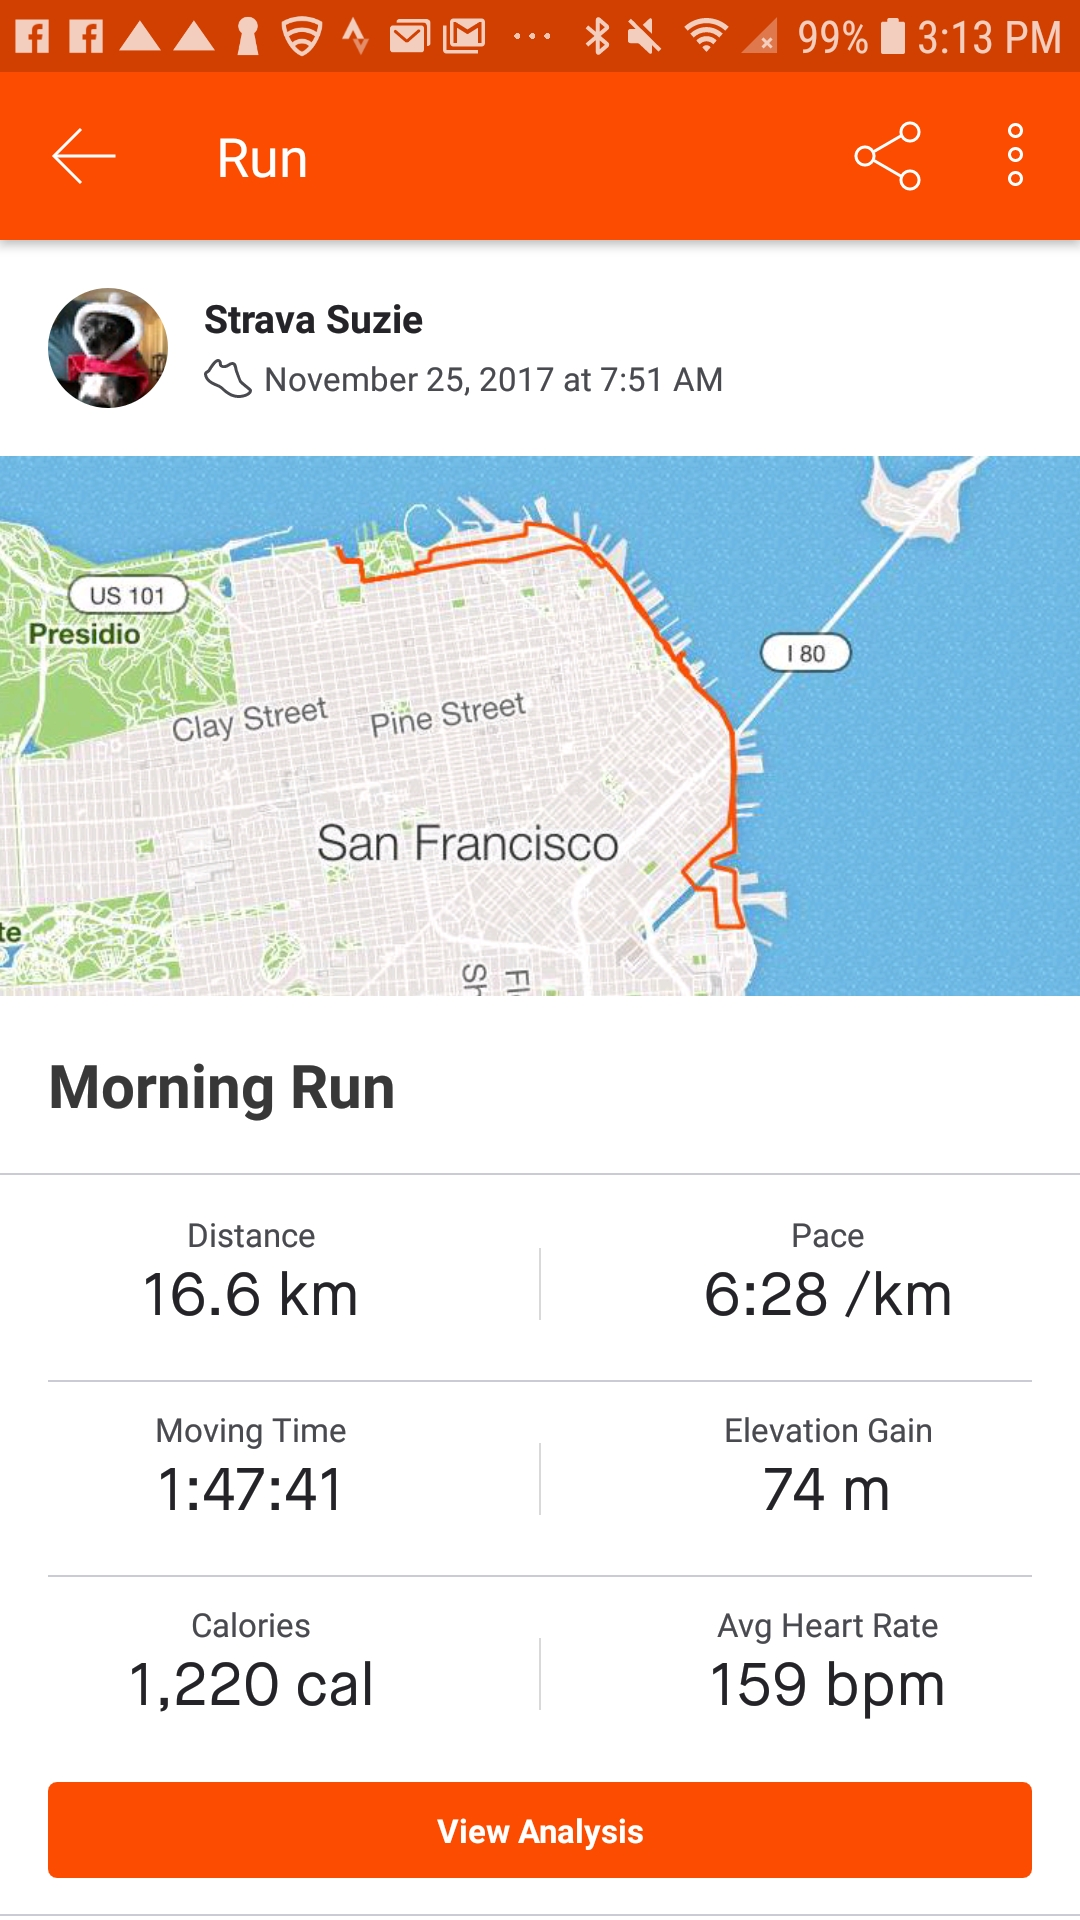
\includegraphics[width=\textwidth]{strava-morning-run-stats.jpg}
    \caption{Statistics of a run on strava\cite{strava-run-stats-img}}
\end{figure}
\subsubsection*{Cross-platform} -- 
\subsubsection*{Propriety} -- 
\subsubsection*{Overall evaluation}

\subsection{myFitnessPal}
https://www.myfitnesspal.com/
\subsubsection*{Use of IoT possibilities} --
\subsubsection*{User fitness assessment} --
\subsubsection*{Availability} --
\subsubsection*{Community} -- 
\subsubsection*{Extra features} -- 
\subsubsection*{User-friendliness} -- 

\begin{figure}[h]
    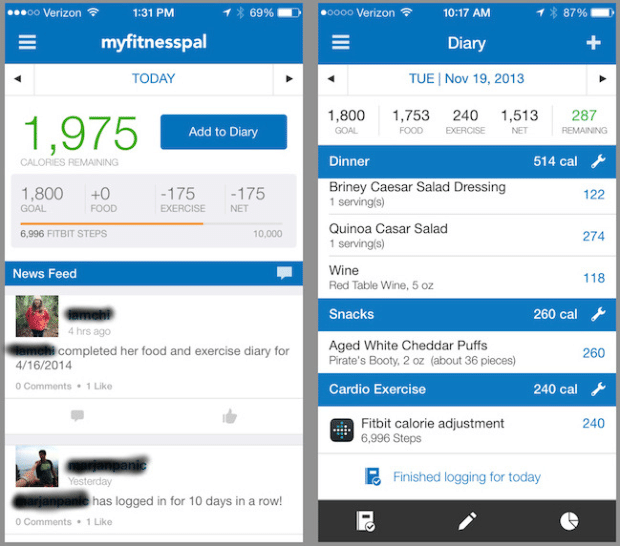
\includegraphics[width=\textwidth]{myfitnesspal-researchgate.png}
    \caption{myFitnessPal feed and diary entry\cite{MFP-diary-img}}
\end{figure}

\subsubsection*{Cross-platform} -- 
\subsubsection*{Propriety} -- 
\subsubsection*{Overall evaluation}

\subsection{Walk with Map My Walk}
https://www.mapmywalk.com/
\subsubsection*{Use of IoT possibilities} --
\subsubsection*{User fitness assessment} --
\subsubsection*{Availability} --
\subsubsection*{Community} -- 
\subsubsection*{Extra features} -- 
\subsubsection*{User-friendliness} -- 

\begin{figure}[h]
    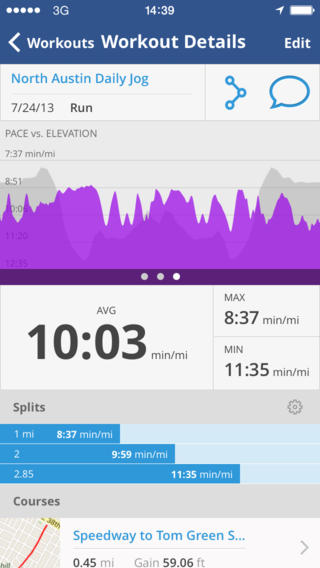
\includegraphics[width=\textwidth]{map-my-fitness-workout-details.jpg}
    \caption{Map my Fitness workout details\cite{map-my-walk-img}}
\end{figure}


\subsubsection*{Cross-platform} -- 
\subsubsection*{Propriety} -- 
\subsubsection*{Overall evaluation}

\subsection{Garmin Explore and Garmin Connect}
The vast ecosystem Garmin has created for their users is filled with an assortment of wearables, radars, smart lights, navigations, customized maps, and plenty more, providing features which are presented to the user via modular mobile apps.

Here I will analyse the Garmin Explore application, which is targeted at hikers, in tandem with Garmin Connect, which functions as a fitness tracker.

\subsubsection*{Use of IoT possibilities}
Most fitness-focused Garmin watches do have a heart rate sensor and all of them include a step counter, however, this data is never compared with that of other users, keeping focus on the user's activity history with no prediction.
\subsubsection*{User fitness assessment}
Some of the heart-rate-monitor enabled watches allow a user to set the zones in which they would like to keep their heart rate depending on the activity they choose to do. The standard zones are:
\textit{
\begin{itemize}
    \item Zone 1 (Warm Up) --
    Perceived exertion: Relaxed, easy pace, rhythmic breathing. Benefits: Beginning-level aerobic training, reduces stress.
    \item Zone 2 (Easy) --
    Perceived exertion: Comfortable pace, slightly deeper breathing, conversation possible. Benefits: Basic cardiovascular training, good recovery pace.
    \item Zone 3 (Aerobic) --
    Perceived exertion: Moderate pace, more difficult to hold conversation. Benefits: Improved aerobic capacity, optimal cardiovascular training.
    \item Zone 4 (Threshold) --
    Perceived exertion: Fast pace and a bit uncomfortable, breathing forceful. Benefits: Improved anaerobic capacity and threshold, improved speed.
    \item Zone 5 (Maximum) --
    Perceived exertion: Sprinting pace, unsustainable for long period of time, labored breathing. Benefits: Anaerobic and muscular endurance, increased power.\cite{garmin-heart-zones}
\end{itemize}
}

\begin{figure}[h]
    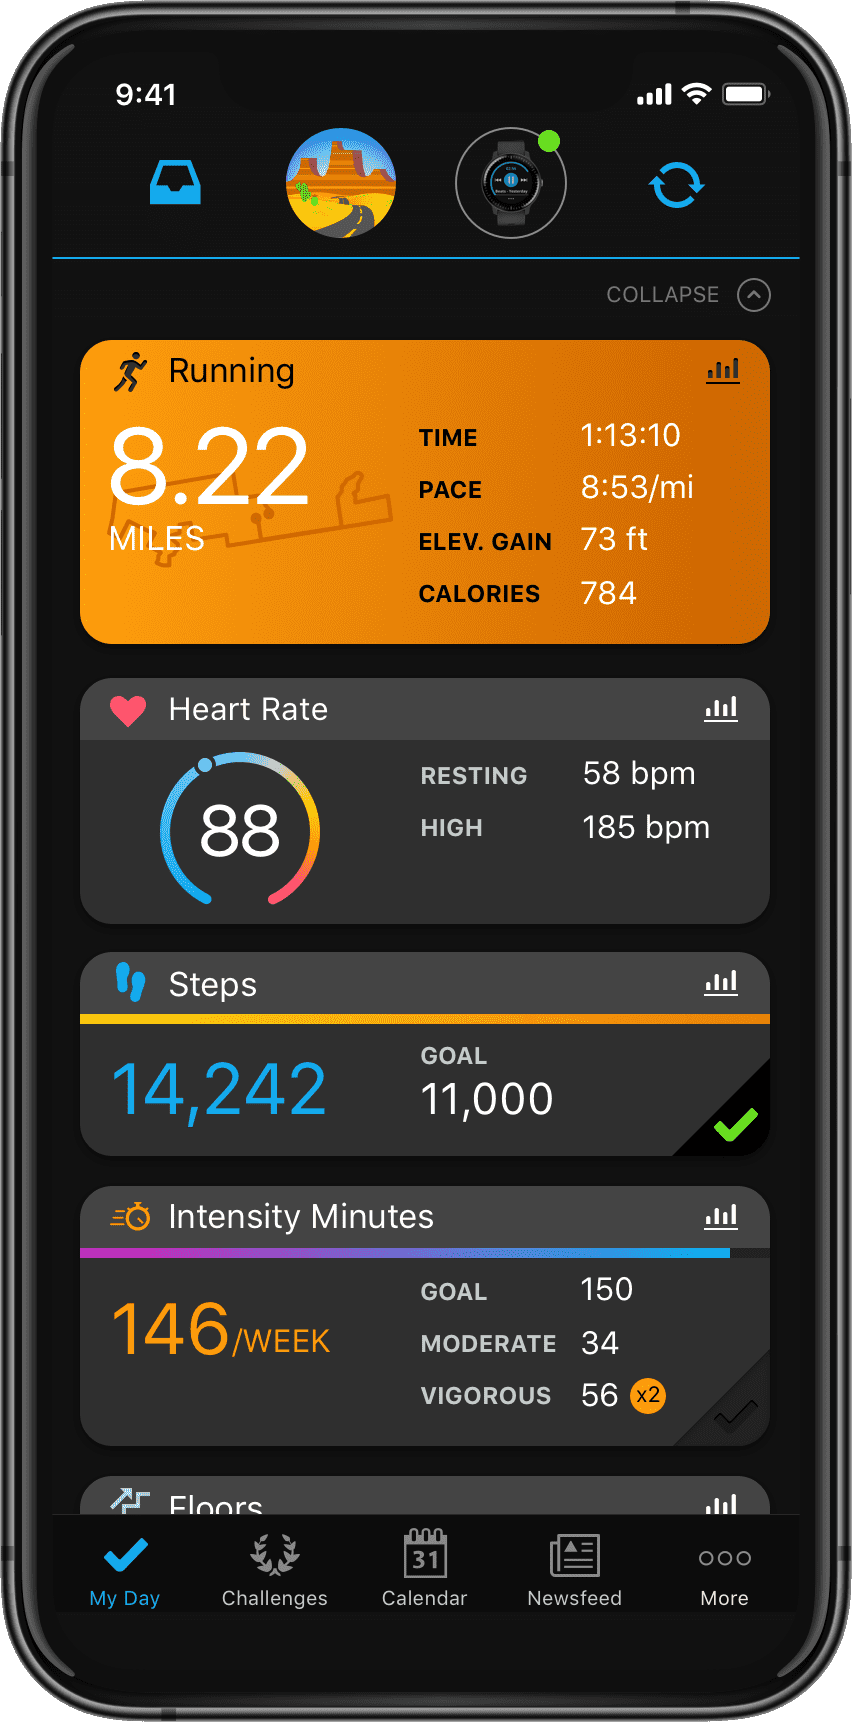
\includegraphics[width=\textwidth]{garmin-connect-myday-screen.png}
    \caption{My day - Garmin Connect's home screen displays statistics of the user's recent activity\cite{garmin-my-day-img}}
\end{figure}

\subsubsection*{Track difficulty assessment}

\subsubsection*{Availability}
In general, Garmin's pricing model relies on the user buying one of their high-end smartwatches, whereupon the rest of the components (apps, basic maps, support, etc.) are free, with some exceptions, such as advanced maps. 
The company's smartwatches are considered premium quality, with a wide price range - target groups include \textit{potential Rolex buyers}\cite{garmin-expensive} as well as ordinary users.\cite{garmin-watches-review}
\subsubsection*{Community}
The Connect application handles the data from the point of view of a fitness tracker, with social features like groups, competitions, likes, comments, and badges of accomplishment.\cite{garmin-connect}
\subsubsection*{Extra features} -- 
\subsubsection*{User-friendliness}

\subsubsection*{Cross-platform}
All of Garmin's applications can be installed both on Android and iPhone.
However, they can only be paired with watches inside Garmin's ecosystem, which is a drawback for users who already own a smartwatch.
\subsubsection*{Propriety}
Some of the Garmin applications are completely open-source, either due to the software that they are derived from, or simply to provide the general public with opportunity to customize their Garmin experience.\cite{garmin-open-source}\cite{garmin-connect-github-repos}
These apps are mostly concerned with map handling, navigation and sound codecs, but also include some bits of functionality like widgets, low power watch apps and others.

While some of this code may be used in the Explore or Connect applications, these repositories don't contain their core functionality.

\subsubsection*{Overall evaluation}
As a fitness tracker, Garmin Connect can definitely be considered acceptable...

\chapter{Functionality}
I decided to construe the user-focused features as one would in a real-life agile project,
as this is in my experience more straightforward and easier to alter when necessary than flooding the reader -- for example, a developer -- with a long list of elaborate use cases right away.
The discussions that take place before reaching a specific decision should be well documented -- brief enough and detailed enough at the same time to provide good value after a quick read.
If the reader has access to a good transcript of these discussions, it is less likely that they will misunderstand the requested functionality;
in the best-case scenario, if the reader is the potential developer, they are an active part of those discussions, so they have a substantial impact on the outcome, thus diminishing the ``coding monkey'' phenomenon.

The top-down approach of the agile methodology which is perhaps the most common and natural to grasp is creating epics, decomposing them into user stories,
and with good knowledge of the project's architecture and after due consideration, adding technical subtasks in an issue tracker of choice.

Epics are complex, high-level characterizations of desired functionality, which usually take longer to deliver than a few weeks.
An epic is usually comprised of description and multiple user stories, which cover the extent of the epic in higher granularity.
Once all the stories are delivered, the whole epic is considered finished.
Epics are sometimes formulated using the same format as user stories.

User stories (US) are short, simple descriptions of a feature told from the perspective of the person who desires the new functionality, usually a user of the system~\cite{user-story-definition}.
They are not system specifications or functional requirements.
Rather, they are the beginning of a conversation that can lead to such specifications or requirements.
However, they provide context and scope of the requested feature.
Often they are written in simple, non-technical language, as most systems do not have tech-savvy users.
The typical template for a user story is:
\textit{As a < type of user >, I want < some goal >, so that < some reason >}~\cite{user-story-definition}, where the reason part is optional but recommended.
Another important component of a US are \textit{acceptance criteria}, which define the functionality which needs to be working for the story to be finished, often including not only the happy path, but a sad path as well.
In general, acceptance criteria should be testable, which is why they are often used as starting points by testers, to get a better idea of what has been done, and provide them with some inspiration.

Based on the analysis of existing solutions, I will now describe the most important features that should be provided by my software.

The main focus of this chapter will be to document my internal analytical discussions.
I will always start with a high-level description of the requested feature formulated as an epic or a user story and elaborate on its details incrementally, summing all of this up in acceptance criteria.
Some stories will also contain hints toward completion for the potential developer, which will be based on research done in previous parts of this thesis.
Since a part of this thesis will focus on implementing a proof of concept, some of the most imperative stories will also be fully processed and finished.

The platform will be referred to as the APP.

%================================================================================================================================
\section{Heart rate monitoring}\label{epic:HRM}
The application should monitor a user's heart rate unobtrusively and reliably.

The user needs a method for getting their data to the mobile application and then to the backend, do it comfortably, preferably without any need for direct user---computer interaction.

\subsection{Manage devices paired with the APP}\label{US:HRM-device-management}
\begin{quote}
As an APP user, I want to pair and unpair my wearables with the APP, so that the APP can use the data of all devices that I currently own.
\end{quote}
The app should provide the user with the list of the phone's paired devices, so that they can choose their fitness gadgets to use on their next hike.
However, since the APP can only support some wearable vendors, the ones that are not compatible should not be pairable.
Also, if this is programmatically possible, non-wearables should not be displayed in the list, or at least should not be pairable,
so that the user does not get confused by the presence or pairability of their Bluetooth speaker.

\paragraph*{Acceptance criteria}
\begin{quote}
    \begin{itemize}
        \item The user can pair any number of compatible wearables.
        \item The user can unpair any number of compatible wearables down to zero.
    \end{itemize}
\end{quote}

\subsection{Activate a device}\label{US:HRM-device-activate}

\begin{quote}
As an APP user, I want to mark a wearable I'm using as active, so that only its data is relevant to the statistics.
\end{quote}

The user should be able to activate a device they want to use for monitoring of current activity or activity in the near future.

\paragraph*{Acceptance criteria}
\begin{quote}
\begin{itemize}
    \item The user can mark a device as active.
    \item When a device is active, the platform can receive data from it.
    \item The user can mark a device as inactive.
    \item Only one device at a time is active; if activating a new one, the old device must be deactivated.
\end{itemize}    
\end{quote}

\subsection{Choose and integrate a wearable}\label{US:HRM-device-integrate}
\begin{quote}
As an APP user, I want my heart rate-enabled wearable to work with the APP, so that I do not have to buy a new one.
\end{quote}

Based on the analysis of existing applications, the most often used type of wearable tech are smartwatches.
While most applications support other devices, such as chest straps, watches are the most convenient and wide-spread gadgets to be used by the general public.
There are a few quite popular smartwatch vendors, most of whom have proprietary protocols of communicating with the system for data processing.
At the time of writing, however, Garmin seems like the most popular option, in spite of being more than a little costly.


\paragraph*{Acceptance criteria}
\begin{quote}
\begin{itemize}
    \item A popular kind of wearables can communicate with the APP in both directions.
\end{itemize}
\end{quote}

It will be more difficult to integrate some devices.
Some vendors do not disclose their devices' API, or the API's documentation is only available for use exclusively by partners of the given vendor,
some do not get paired with the phone itself and communicate with a proprietary app using server-based pairing instead (such as the Xiaomi Mi Band 4 I initially intended to use in the PoC) and there is no easy or straightforward way to get the data.
For example, getting data from the Mi Band 4 would require root access to the user's phone~\cite{miband4-server-based}, which is just not an option for a normal user.
Therefore I recommend limiting the supported devices to those that do not use server-based pairing, as this would cover most of the currently available gadgets,
or take advantage of (and contribute to) existing open-source software for wearables integration, such as Gadgetbridge~\cite{Gadgetbridge}.
By building on existing integrations it will be easier to spread across the market.

In addition to these restrictions, continuous heart rate monitoring causes an extreme drain of the watch's battery, which is fine for short activities (sprints, swimming, cardio workouts), but can be a considerable issue while hiking.
This is why I recommend supporting mostly devices which have a large capacity in this regard.

For my PoC in this thesis, I chose the XXXXXXXXX.\todo{add what and why}

%================================================================================================================================

\section{Objective user fitness assessment}\label{epic:fit}
\begin{quote}
As an APP user, I want my fitness to be assessed, so that I can get relevant estimations of route difficulty.
\end{quote}

Having analyzed the conventional ways of user fitness assessment in a previous chapter, the application should allow a user to use one of the multiple ways to get their fitness level.
The outcome of the assessment should be the individual's VO2 max index and their heart rate zones -- so that if they need to maintain their heart rate in a specific range, they can cross-reference it with the exhaustion they perceive and learn to recognize when they are in the desired zone.

If the user has no physical impairments, they can have their HR max assessed by a simple age-based formula, such as the one developed by Nes et al. (see the chapter on fitness assessment).

Users with physical impairments could self-evaluate how much their condition affects their fitness, and based on this their HR max can be set by using one of the standard formulas and subtracting a smaller or larger number of beats per minute (further research needs to be done on how many beats this should be).
This self-assessed value should be corrected as more data is available about the user.

As far as objective assessment, I see plenty of potential for the use of machine learning and neural networks.
The networks can learn from the data collected from a good number of users over a longer period, and then categorize the new users into fitness groups based on this data, which will then be used to predict the users' future hikes.

\subsection{Implement support for VO2 max tests}\label{US:fit-vo2max}
\begin{quote}
As an APP user, I want to be able to take a guided test of my fitness in the APP, so that I do not have to look for tests elsewhere.
\end{quote}

The APP should implement a guide to multiple tests of VO2 max, with instructions on what they should do, and signals to direct the user while taking the test.
The instructions should also contain a description of the signals the user will receive.
The initial instructions should be textual and possibly audible, so that the user understands the aim of the test before taking it.
During the test, a watch vibration should alert the user about an incoming signal which will be displayed on the watch.
This signal would contain directions like 'Turn in N seconds' where N is a countdown to 'Turn now!'.
When no signals are occupying the device's screen, there should be pep talks like 'Keep going!' and 'Great job!'.
At all times during the test, there should be the test status on the device's screen: remaining time, distance walked, and any other metric relevant to the test.

As it is the most accurate of the more feasible tests, the application should encourage the user to take the 6-Minute Walking Test, and let them take it using the app in both 15- and 30-metre-long variations.
In order to calculate VO2 max, the APP can use Mänttäri's formulas.

\paragraph*{Acceptance criteria}
\begin{quote}
\begin{itemize}
    \item The user can take at least one VO2 max test using the APP.
    \item During the test, the user gets directions on their smartwatch.
\end{itemize}
\end{quote}

\subsection{Implement support for HR max and HR min tests}\label{US:fit-HR}
\begin{quote}
As an APP user, I want to be able to take a guided test to find my heart rate zones in the APP, so that I do not have to look for tests elsewhere and get as accurate heart rate zones as possible.
\end{quote}

The implementation should be similar to VO2 max tests; if possible, both metrics should be measured by a single test to reduce the time a user has to spend setting up the APP.

\paragraph*{Acceptance criteria}
\begin{quote}
\begin{itemize}
    \item The user can take at least one HR max test using the APP.
    \item The user can take at least one HR min test using the APP.
    \item During the tests, the user gets directions on their smartwatch.
\end{itemize}
\end{quote}

%================================================================================================================================

\section{Manual input of biometric data}\label{epic:manual}

The users might not want to take an exhausting test at the time of setting up the APP.
This is why they should be allowed to input the data in other ways.

If a public universal database with all people's medical data existed, it would make sense to get the necessary information directly via an API.
However, as no such thing exists (and for good reasons), we will let the user enter their biometric data manually.

\subsection{Allow manual input of basic biometric values}\label{US:manual-basic}
\begin{quote}
As an APP user, I want to provide the APP with my basic metrics, so that the results are relevant to me.
\end{quote}

If the user has a smart scale, it could be integrated to get the most recent values, however, that seems like a bit of an overkill, considering that it's just one number - the weight.

The APP needs the user's height, weight, biological sex and age.
The age should be calculated based on their date of birth, so that it is always reasonably accurate.
However, I myself have had issues with disclosing my exact date of birth to just any application that asks for it, and the accuracy would be good enough with even just the month and year.
Yet again, it is reasonable to consider whether a user who does not have an issue giving out their heart rate and fitness data would show similar concern.

\paragraph*{Acceptance criteria}
\begin{quote}
\begin{itemize}
    \item User can enter their basic metrics - height, weight, age, sex - manually.
\end{itemize}
\end{quote}

\subsection{Allow manual input of advanced biometric values}\label{US:manual-advanced}
\begin{quote}
As an APP user who has recently done lab fitness tests, I want the APP to use these values instead of taking the APP's tests, so that I do not have to take fitness tests that are most probably less accurate than what I know.
\end{quote}

A user should be able to manually enter the VO2 max, resting heart rate and maximum heart rate, as well as the severity of the effect a potential condition might have on the individual's fitness.
The APP should ask whether the user has such a condition and if there is a maximum heart rate (perhaps recommended by a doctor) the user should not exceed when active.

\paragraph*{Acceptance criteria}
\begin{quote}
\begin{itemize}
    \item User can enter their advanced biometric data - VO2 max, HR max, HR min - manually.
    \item The APP asks about the severity of any conditions that the user has and its impact on their fitness.
    \item The APP asks about a recommended maximum heart rate the user should not exceed.
\end{itemize}
\end{quote}

%================================================================================================================================

\section{Routes and maps}\label{epic:map}

\subsection{Integrate a map}\label{US:map-integrate}
\begin{quote}
As an APP user, I want to use a map to visualize my hikes, so that I can follow them easily.
\end{quote}

Since the APP is meant to be used as a hike planner, the user needs an easy to follow aid to help them plan their routes.
The whole APP should be focused around the hikes a user takes and around their difficulty given the user's fitness level.

\paragraph*{Acceptance criteria}
\begin{quote}
\begin{itemize}
    \item An interactive map is displayed in the APP.
\end{itemize}
\end{quote}

There is not a large variety of maps available for use by developers.
While Google Maps would probably be a popular choice, Google decided to put their maps behind a paywall~\cite{google-maps-paywall} in 2018.
Therefore it makes sense to choose the open-source OpenStreetMap~\cite{OpenStreetMap} and use one of its derivatives with a public API for route planning (such as OpenRouteService~\cite{OpenRouteService}).

It is important not to forget to credit the map's creator in their preferred way.

\subsection{Plan a route}\label{US:map-plan}
\begin{quote}
As an APP user, I want to plan a route from point A to point B.
\end{quote}

Hikers often do not want the easiest, fastest, or shortest possible path from A to B -- they look for a challenge and nice things to see.
This is why they might make extra effort to take their hike through a specific spot, which might not be on the ideal route.
Therefore, it should be possible to add such places to the route.

Since there are often multiple ways to get from A to B even through the chosen waypoints, the user should be able to choose which one they want to take.

Another option that is related to route planning is choosing whether or not to plan a round trip.
Especially in hiking, when a lot of people come to the starting point by car, they want to return to the same point where they started.
In order to keep the route interesting, the way back should be different than the way to the destination point, if possible.

\paragraph*{Acceptance criteria}
\begin{quote}
\begin{itemize}
    \item User can pick a starting point from the map.
    \item The user's current location can be automatically found and set as the starting point.
    \item User can choose points on the map through which they want to pass.
    \item User can choose a destination point from the map.
    \item User can remove points from the planned route.
    \item The points in a planned route can be rearranged in any order.
    \item If the last waypoint is removed, the previous waypoint becomes the last point.
    \item If multiple different routes are available, the user can compare their attributes.
    \item If multiple different routes are available, the user can only choose one of them.
    \item Allow the user to do a round trip.
\end{itemize}
\end{quote}

\subsection{History of hikes taken}\label{US:map-history}
\begin{quote}
As an APP user, I want to see which routes I've hiked while using the APP, so that I can remind myself of the impressions of the hike.
\end{quote}

A user might want to remind themselves of a specific hike they went to -- if it's because of fond memories, or just to make sure who went with them, or when it happened.
This is why it's important to keep a log of the hikes the user has taken ever since logging in to the APP.

Every route is planned over a network of geographical coordinates, which means one can create thumbnails from its projection on a map.
This, along with the names of nearby prominent landmarks, such as the mountain range through which the user hiked, and the date of the hike, should be enough for the user to identify the route they were searching for.
Since there is a number of attributes a route can have, it should be possible to filter by them.
Filters should include the date on which the hike was taken, the time it took to complete it, the route's length, and other quantitative attributes.

\paragraph*{Acceptance criteria}
\begin{quote}
\begin{itemize}
    \item Show a filterable list of hikes taken by the user.
\end{itemize}
\end{quote}

\subsection{Saved routes}\label{US:map-saved}
\begin{quote}
As an APP user, I want to save some routes, so that I can do not have to create the same route again when I want to retake it.
\end{quote}

Since the process of creating a route from scratch is somewhat lengthy, the user should be able to save it and find it later.

\paragraph*{Acceptance criteria}
\begin{quote}
\begin{itemize}
    \item User can plan a brand new route and save it.
    \item User can choose an existing route made by their friend and save it.
    \item User can remove a route from saved routes.
    \item User can choose a saved route and hike it again.
\end{itemize}
\end{quote}

\subsection{Share routes}\label{US:map-share-route}
\begin{quote}
    As an APP user, I want to link routes, so that I can discuss with my friends if we want to take it.
\end{quote}

A group of friends is likely already using some sort of messaging, so sharing a link to the route and its details can make discussions about where to go faster.

\paragraph*{Acceptance criteria}
\begin{quote}
    \begin{itemize}
        \item User can get a link to a route.
        \item When the link is opened, the route's details are shown.
    \end{itemize}
\end{quote}

A group of friends is likely already using some sort of messaging, so sharing a link to the route and its details can make discussions about where to go faster.

\paragraph*{Acceptance criteria}
\begin{quote}
    \begin{itemize}
        \item User can get a link to a route.
        \item When the link is opened, the route's details are shown.
    \end{itemize}
\end{quote}

\subsection{Display planned route details}\label{US:map-planned-details}
\begin{quote}
As an APP user, I want to see interesting information about a route that has been planned for me, so that I can make an informed decision whether or not to take it.
\end{quote}

When tapping a route, its details should be shown: its outline on a map, length, terrain in its segments, its elevation profile, colours of each official hiking route it uses, and interesting places to see along the route.
This is also the place for information that is customized for the user's fitness -- such as how long it will probably take them to hike it, how difficult its segments will be for the user in terms of perceived exertion and expected heart rate zones.
This should take into account the limitations of the user's fitness, which they may have entered according to \ref{US:manual-advanced}.

\paragraph*{Acceptance criteria}
\begin{quote}
\begin{itemize}
    \item User can interactively see basic details of a planned route, including the route on a map, its length, terrain analysis, and elevation profile.
    \item User can see customized biometric details of a planned route, including the amount of time the hike will take them, the relative difficulty of the route's segments, and expected heart rate zones.
\end{itemize}
\end{quote}

\subsection{Display old hike details}\label{US:map-old-details}
\begin{quote}
As an APP user, I want to see interesting information about a route I've hiked, so that I can check it in a few days and show my friends.
\end{quote}

\paragraph*{Acceptance criteria}
\begin{quote}
\begin{itemize}
    \item User can see all the basic info as on a planned route.
    \item User can see the originally estimated values of biometric indicators and real values.
    \item User can see a graph of their heart rate during the hike.
\end{itemize}
\end{quote}

\subsection{Hike a route}\label{US:map-hike}
\begin{quote}
As an APP user, I want to hike the route that I planned before.
\end{quote}

Navigation is a core feature of this APP since the planned hike is almost useless if the user cannot follow it in the APP.
But since it is not the only important feature, it should also be possible to temporarily escape the navigation mode, so that the user can do other things in the APP.

\paragraph*{Acceptance criteria}
\begin{quote}
\begin{itemize}
    \item User can start a planned hike on the day it was planned for.
    \item User can follow the directions of the APP to stay on track.
    \item Once the destination is reached, navigation mode is automatically turned off.
    \item The navigation mode can be temporarily put in the background to use other parts of the APP.
    \item Information about current segment is shown -- the slope, the user's heart rate zone.
    \item While hiking, the user can see if they're following the plan -- whether they're on time, or should go faster.
\end{itemize}
\end{quote}

\subsection{Change the hike date}\label{US:map-hike-change}
\begin{quote}
As an APP user, I want to replan my existing planned hike to a different day, so that if the weather is bad, I do not have to cancel it and plan all of it again.
\end{quote}

\paragraph*{Acceptance criteria}
\begin{quote}
\begin{itemize}
    \item User can change the date of a planned hike they have planned.
\end{itemize}
\end{quote}


%================================================================================================================================

\section{User profile}\label{epic:user}
\begin{quote}
The user needs a place to review and change their provided information, as well as a possibility to take the provided tests.
\end{quote}

\subsection{Management of provided biometric information}\label{US:user-manage-info}
\begin{quote}
As an APP user, I want to be able to change the information I've entered into the APP, so that the values are always up to date and my estimates remain accurate.
\end{quote}

\paragraph*{Acceptance criteria}
\begin{quote}
\begin{itemize}
    \item User can add and delete weight entries.
    \item User can edit the height entry, the recommended maximum heart rate, and the severity of potential health conditions.
    \item User can edit the advanced biometric data.
\end{itemize}
\end{quote}

\subsection{Profile picture management}\label{US:user-manage-pic}
\begin{quote}
As an APP user, I want to be able to upload and delete my profile picture or use one from social media, so that my friends can recognize me in their friends list quickly.
\end{quote}

\paragraph*{Acceptance criteria}
\begin{quote}
\begin{itemize}
    \item If the user does not have a profile picture, there is a substitute placeholder.
    \item User can upload a profile picture.
    \item User can see the new profile picture once uploaded.
    \item User can delete their uploaded profile picture, which is replaced by a placeholder.
\end{itemize}
\end{quote}

\subsection{Log in options}\label{US:user-log-in}
\begin{quote}
As an APP user, I want the APP to recognize me on different devices, so that my data is still connected to me when I change my phone.
\end{quote}

People change their phones every few years, some even months, but want their new phone to have all the data as the old one.
This can be done with manual backups.
However, since our APP has a server where most of the data is stored anyways, the data should be linked to the person's account and not the phone.
The user should be able to sign up with e-mail, as well as social media platforms so that multiple user groups are targetted.

I considered allowing the user to use the APP without an account, at the risk of them losing all their data, but it would not only be a nuisance for the user --
a lot of processing power would have to be reinvested into the same user, and the previous data would not be as useful as they could be.

\paragraph*{Acceptance criteria}
\begin{quote}
\begin{itemize}
    \item User can create an account using their e-mail.
    \item User can create an account using at least one social media platform.
    \item User can sign in to the same account on different devices and see all their data.
\end{itemize}
\end{quote}

%================================================================================================================================

\section{Hike with friends}\label{epic:friends}

Since hiking is generally an activity for small groups of people, it makes sense to be able to create groups in which everybody will know the hike's details and will be able to navigate.

Here I was able to discern between two main use cases -- on the one hand, a user knows what is the group of friends they want at the hike and wants to just find a good route,
and on the other hand, they want to hike a specific route and want the right people to join in.
There is a third use case, the mix of the previous two, where the hike host knows about some people they want at the hike (for example their spouse) and would just like people to join in if they want to.

\subsection{Adjust the calculations to friends' fitness}\label{US:friends-fitness}
\begin{quote}
As an APP user, I want the estimations to be accurate even if I'm hiking with friends.
\end{quote}

In a diverse group of people, someone's fitness level will likely be lower than that of the others, which means that the whole hike will take longer than if this person was not in the group.
This is why the estimated time spent on the hike should be calculated based on the weakest link, and each participant's expected heart rate zones and all other biometric estimations should be adjusted accordingly.

The estimations can be adjusted either to the weakest participant's capabilities, or the system can acknowledge the motivation that they will feel when with others and slightly overestimate.

It would not be user-friendly to expose the name of the weakest individual, as they might feel ostracised, disheartened and less likely to go on hikes with their friends for fear of holding them back
(and, by extension, stop using the APP that made them feel that way).
But at the same time, the aim of the solution is to provide accurate estimations for its users.
This is why it should provide the information carefully.

\paragraph*{Acceptance criteria}
\begin{quote}
\begin{itemize}
    \item When a hike is planned for a group of people, the predicted total time should be based on the time it would take the least fit user.
    \item The biometric values such as heart rate zones should be recalculated for all participants based on the total time the hike should take.
\end{itemize}
\end{quote}

%==========Invite friends to hikes======================================================================================

\subsection{Invite friends to hikes}\label{US:friends-invite}
\begin{quote}
As an APP user, I want to invite friends to my hikes, so that we all have access to the same track when hiking it and preparing for it.
\end{quote}

The invitation should include the proposed date of the hike and all the hike's details, including the time the hike will take if the user joins the group.

\paragraph*{Acceptance criteria}
\begin{quote}
\begin{itemize}
    \item When user A is planning a hike, they can invite their friend user B to join. 
    \item When user A invites user B to a hike, user B receives an invitation with the hike's details.
\end{itemize}
\end{quote}

\subsection{Refuse an invitation to hike with friends}\label{US:friends-invite-refuse}
\begin{quote}
As an APP user, I want to refuse invitations to hikes that I do not want to attend, so that the hike organiser knows I will not come and my invitation list is not cluttered.
\end{quote}

\paragraph*{Acceptance criteria}
\begin{quote}
\begin{itemize}
    \item When user A receives an invitation from user B, user A can refuse the invitation.
\end{itemize}
\end{quote}

\subsection{Accept an invitation to hike with friends}\label{US:friends-invite-accept}
\begin{quote}
As an APP user, I want to accept invitations to hikes that I want to attend, so that I get updates and plan around the event.
\end{quote}

\paragraph*{Acceptance criteria}
\begin{quote}
\begin{itemize}
    \item When user A receives an invitation from user B, user A can accept it. From then on, user A is an active participant of the hike.
\end{itemize}
\end{quote}

%=============Friends and friendship request management================================================

\subsection{Add friends}\label{US:friends-add}
\begin{quote}
As an APP user, I want to add new friends, so that I can invite them to hikes.
\end{quote}

The only people that can be added, need to be users of the system.
In order to add friends, the APP can use user profile links (primarily textual, but QR codes could be a popular option) and social media.
A nice-to-have way would be using the phones' proximity if the two people are close to one another, for example with Bluetooth or NFC.

\paragraph*{Acceptance criteria}
\begin{quote}
\begin{itemize}
    \item User A can send a friendship request to user B via a link to user A's profile.
    \item User A can send a friendship request to user B via popular social media.
    \item If the request is accepted, user A can invite user B to hikes and vice versa.
\end{itemize}
\end{quote}

\subsection{Remove friends}\label{US:friends-remove}
\begin{quote}
As an APP user, I want to remove people I no longer meet with from friends, so that they cannot invite me to hikes anymore.
\end{quote}

\paragraph*{Acceptance criteria}
\begin{quote}
\begin{itemize}
    \item If user A and user B are friends, both can remove the other user from their list of friends.
    \item If user B is removed, neither user A or user B can see each other's profiles or invite each other to hikes.
    \item If user B is removed, the hikes (and related data) user A and user B took together remain in their respective histories.
\end{itemize}
\end{quote}

\subsection{Accept a friendship request}\label{US:friends-accept}
\begin{quote}
As an APP user, I want to accept a friendship request that someone sent me, so that we can invite each other on hikes.
\end{quote}

\paragraph*{Acceptance criteria}
\begin{quote}
\begin{itemize}
    \item When user A sends a friendship request to user B, user B can accept the request.
    \item When user B accepts a friendship request from user A, they can both invite each other for hikes.
    \item When users are friends, they cannot send new friendship requests to each other.
\end{itemize}
\end{quote}


\subsection{Dismiss a friendship request}\label{US:friends-dismiss}
\begin{quote}
As an APP user, I want to dismiss a friendship request when I do not know the sender or do not want to hike with them, so that my request list is not cluttered.
\end{quote}

\paragraph*{Acceptance criteria} 
\begin{quote}
\begin{itemize}
    \item When user A sends a friendship request to user B, user B can dismiss the request.
    \item When user B dismisses a friendship request from user A, neither of them can invite the other one for hikes.
    \item When user A sends a friendship request to user B, user B cannot send a friendship request to user A; they can only accept or dismiss the existing request.
\end{itemize}
\end{quote}

\subsection{Share a link to a profile}\label{US:friends-share}
\begin{quote}
    As an APP user, I want to share my and my friends' profiles, so that we can connect more easily.
\end{quote}

\paragraph*{Acceptance criteria}
\begin{quote}
    \begin{itemize}
        \item User A can share a link to their own profile.
        \item User A can share a link to their friends' profiles.
    \end{itemize}
\end{quote}

%=======Joinable hikes=======================================================================================================

\subsection{Joinable hikes}\label{US:friends-join-hikes}
\begin{quote}
As an APP user, I want to let my friends join my hikes, so that if I do not know who exactly I want there, my friends can decide for themselves if they want to come and I do not have to text everybody myself.
\end{quote}

When planning a hike, not always do we know who might want to come, and sometimes we really want to try out a specific route.
This is why the APP should allow the user to not only invite people, but also allow the user's friends to join if they want to.
The user's friends need to find out about the upcoming plans, this is why the APP should have a feed of the community's plans.

At the same time, if the hike is already meant to be long, the user will not want someone to simply join because they want to, if it should mean extra two hours added to the total time.
That is why the potential participant's request should be reviewed by the hike's host.
This request should let the host know how much time this new person would add to the hike.

To look at this from the side of the requester, they should also be able to tell if the hike is going to be too hard for them, and whether them joining would make the hike ridiculously long.

Another point to consider is the capacity of such a hiking trip -- the hike's host should be able to stop the joining requests when they've decided there are enough or the right people, and receive them again if somebody cancels.

\paragraph*{Acceptance criteria}
\begin{quote}
\begin{itemize}
    \item When planning a hike, it can be marked as joinable.
    \item User can see their friends' upcoming plans and their difficulty, relative to this user's fitness.
    \item User A can ask to join user B's joinable hike.
    \item When user B receives a request from user A to join one of their hikes, they can see how this changes the hike's total time so that they can make an informed decision.
    \item A hike can be marked as \code{not joinable} after being joinable and vice versa.
    \item When a hike is marked as \code{not joinable}, all pending joining applications should be dismissed.
\end{itemize}
\end{quote}

\subsection{Cancelling a hike}\label{US:friends-cancel-hike}
\begin{quote}
As an APP user, I want to let my friends know that I will not be able to go to the hike, so that their metrics are accurate when I'm not there.
\end{quote}

When different plans come up, a user will want to cancel their participation on a hike.
This can happen both to an invited attendee and the hike's host.
This is why it should be possible to appoint a new host from the invited friends if the original host needs to cancel -- there should always be a host.

\paragraph*{Acceptance criteria}
\begin{quote}
\begin{itemize}
    \item When user A accepts an invitation from user B, user A can let user B know that they have changed their mind and will not attend. The total time and the attendees' biometric estimates should be recalculated.
    \item A hike's host can cancel, but they have to appoint a new host.
\end{itemize}
\end{quote}

\subsection{Hike active on all participants' phones}\label{US:friends-hike-active}
\begin{quote}
As a guest on a hike, I want to be able to navigate, so that if the host's phone battery dies, there's someone to keep track of the route.
\end{quote}

\paragraph*{Acceptance criteria}
\begin{quote}
\begin{itemize}
    \item When a hike is started, it is started on the phones of all attendees.
\end{itemize}
\end{quote}

%====================================================================================================================================

\section{Notifications}\label{epic:notif}
Everything important that happens on the APP should have notifications.

\subsection{Notifications for friends tab}
\begin{quote}
As an APP user, I want to receive notifications about friend requests.
\end{quote}

\paragraph*{Acceptance criteria}
\begin{quote}
\begin{itemize}
    \item If user A sends user B a friendship request, user B receives a notification.
    \item If user A sends user B a friendship request and user B accepts, user A receives a notification.
\end{itemize}
\end{quote}

\subsection{Notifications for planned hikes}\label{US:notif-plans}
\begin{quote}
As an APP user, I want to receive notifications about my planned hikes.
\end{quote}

The hike host should receive notifications about activity of this hike: join requests, accepted and refused invitations.

A hike guest should receive notifications about activity of the hike: change in attendance, change of date.

Everybody who attends the hike should get a notification about the hike's planned date coming up soon (for example, in a week, and on the next day).

\paragraph*{Acceptance criteria}
\begin{quote}
\begin{itemize}
    \item If user A requests to join user B's hike, user B receives a notification.
    \item If user A sends user B a join request and user B accepts, user A and user C (another hike guest) receive a notification.
    \item If user A as the host of the hike changes the date of the hike, all attendants except for the host should receive a notification.
    \item If user A's hike is planned to seven days from now, every attendee receives a notification.
    \item If user A's hike is planned next day from now, every attendee receives a notification.
\end{itemize}
\end{quote}

%=========Considered features================================================================================================

\section{Considered features}
One feature that could help make the platform into a social network is messaging.
I decided against it because everybody is already using their messaging apps of choice to communicate and it would be distracting the user from planning their hikes.
However, letting people see their friends' previous hikes and letting them react to all that is happening could be a good community feature.

Some other features that would be interesting to see in the application are
\begin{itemize}
    \item integration with geocaching~\cite{geocaching} for gamification,
    \item showing the weather forecast for the planned day in the details of the hike,
    \item user groups for users who always hike together, so that they would not have to search for their friends every time,
    \item multiple hike hosts, so that there are multiple people who can oversee the hike's activity,
    \item collecting data of non-planned, spontaneous hikes,
    \item cancelling the hike once it has started, so that if the user decides they do not actually want to go, the APP does not force them,
    \item pausing the hike so that the attendees can have a lunch break,
    \item offline maps and navigation,
    \item optional notifications for when the user is not following the plan (when being too slow or wandering off-route).
\end{itemize}


\chapter{Mobile app UI design}
Thanks to the functionality of the platform described in the previous chapter, I was able to create a design for the user interface -- UI of the mobile application.

In the beginning of this UI design project, I first looked at what would be the platform the project should run on.
Since it is a mobile application, the range of options was slimmed down to two -- either Android or iOS,
given their prevalence on the market (Android on the first place with 70.68\% of the market share, iOS second with 28.79\% as of April 2020). \cite{market-share-mobile-os}
It is partially due to Android's crushing lead on iOS devices, but also because of my personal experience with the more popular OS, that I decided to design the app for Android.

One of the most important decisions to make when designing an application is the navigation in it, and from there there's only a small step to information architecture (IA) -- the \textit{science of organizing and structuring content of the [\dots] mobile applications} \cite{information-architecture}.
The IA of an application helps the designer decide which concepts in the application are high-level and discrete enough
to be used as an `umbrella terms' for navigating to other, deeper concepts, while feeling intuitive to the user.

However, when reading up on design guidelines for either of the systems, I realised that Android's instructions seem outdated.
Backed by plenty of discussions online as well as my own user experience with the native applications, the typical hamburger menu ☰ has gone out of style.

One of the reasons is the increasing size of handheld devices.
A hamburger menu (or `navigation drawer') located in the top left corner is nearly inaccessible for the majority of users, who are right-handed and use their thumb to operate the device. \cite{thumb-zone-article} 
\todo{insert pic of thumb zone on small to large phones}

Another reason is the fact that the hamburger menu decreases discoverability of features, as they are hidden by default. \cite{hamburger-discoverabillity}

Lastly, using the hamburger menu often tempts the designer to just put everything there, without giving too much consideration to the use of the features.

One of the most popular alternatives is the tab bar -- or `bottom navigation' in Android documentation.
This type of navigation is mainly implemented by Apple's designers, but is fast spreading to Android-powered devices.
It's a bar on the bottom of the screen containing three to five labelled icons representing \textit{tabs} where each leads to a different location in the app.
It enforces the idea that a user should always know where in the application they are, what they can do there and where they can go because it's always on the screen (except when the keyboard is being used).
Another one of its advantages is the possibility of inobtrusive notifications using icon badges -- little red circles in the top right corner of the icon, often containing a number to show the number of notifications.
Other navigation options include dropdown menus, scrollable menus, single page dot navigation, and others. \cite{hamburger-alternatives}

I chose the tab bar with five tabs: `Plans', `Routes', `Map', `Friends', and `Profile'.
However, when installing the APP, the user needs to set the APP up.

\section{Set up screens}
The welcome screen contains all the options for signing up, with a button to switch to the sign-in screen if the user already has an account.
Signing up with e-mail creates a new account for the user based on their e-mail~(fig.\ref{fig:sign-up-email}), while using a social network account takes the user to a sign-in screen of the specific social network.
Similarly, the user can sign in to their existing account~(fig.\ref{fig:sign-in-email}).

\begin{figure}[h!]
    \centering
    \tmpframe{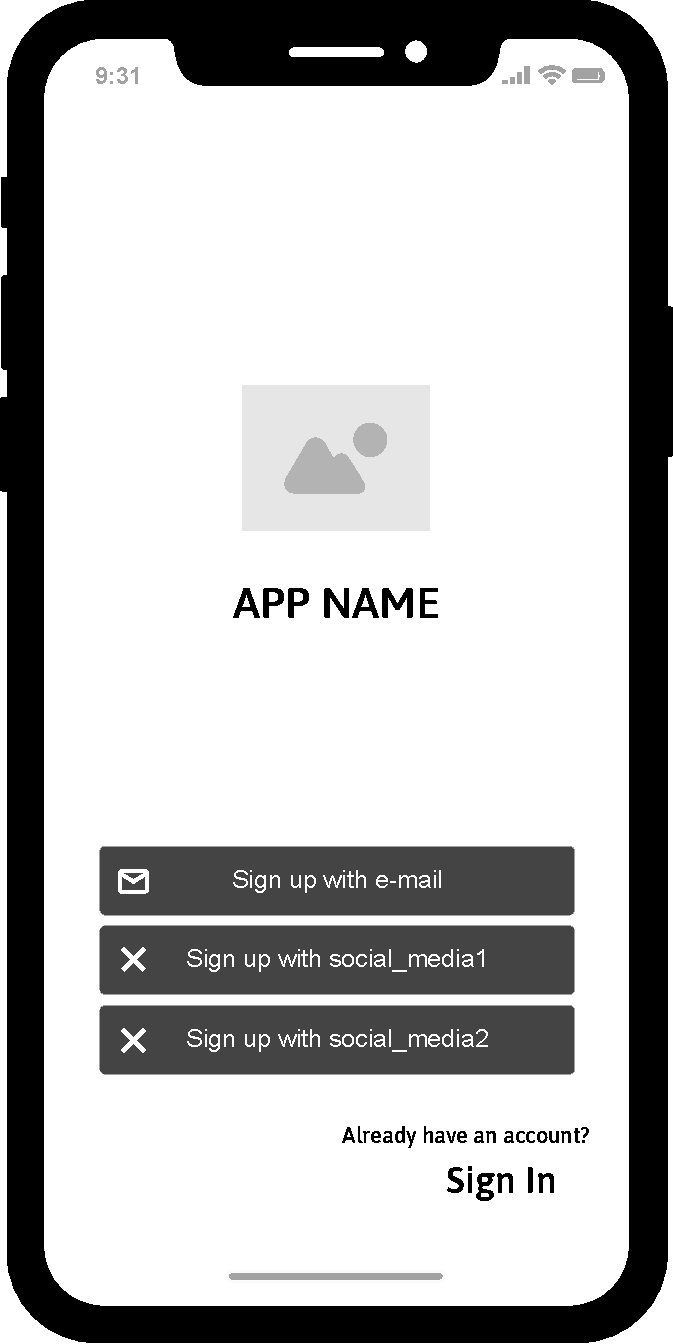
\includegraphics[width=0.4\textwidth]{Images/appScreens/signUp1.pdf}}\hfill
    \tmpframe{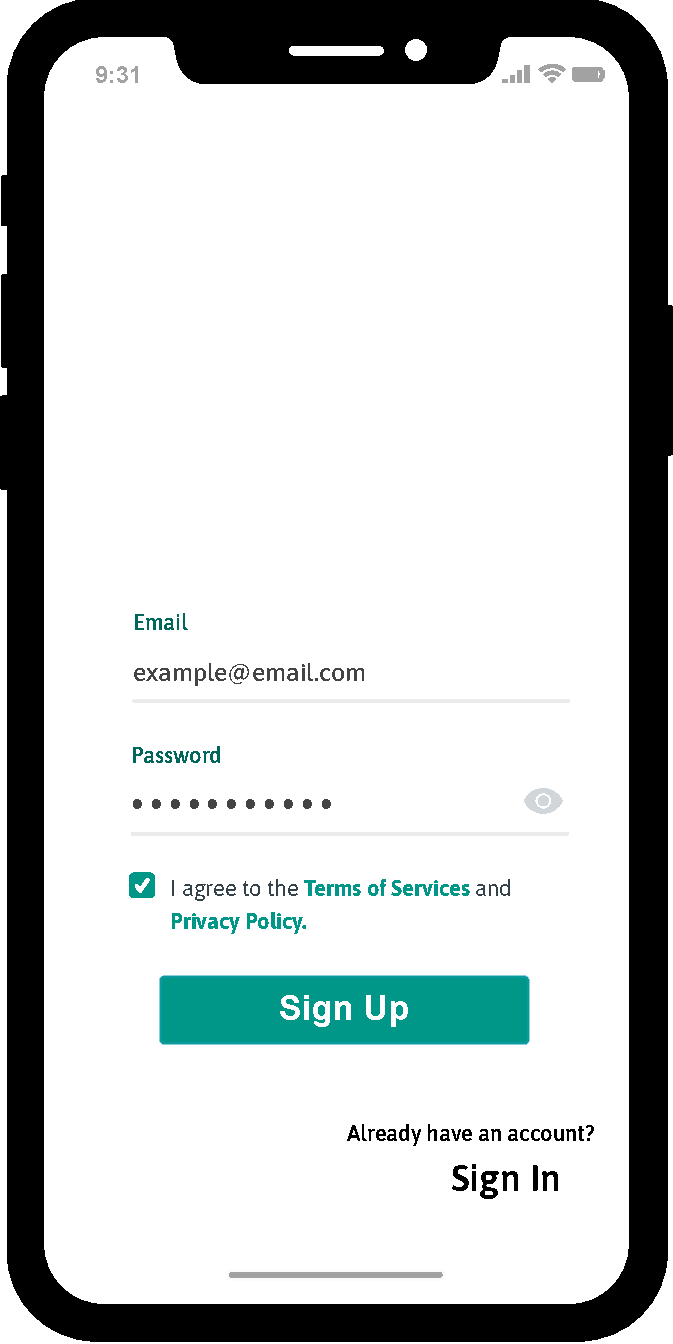
\includegraphics[width=0.4\textwidth]{Images/appScreens/signUp2.pdf}}
    \caption{Welcome screen with sign-up options and e-mail sign-up screen}
    \label{fig:sign-up-email}
\end{figure}

\begin{figure}[h!]
    \centering
    \tmpframe{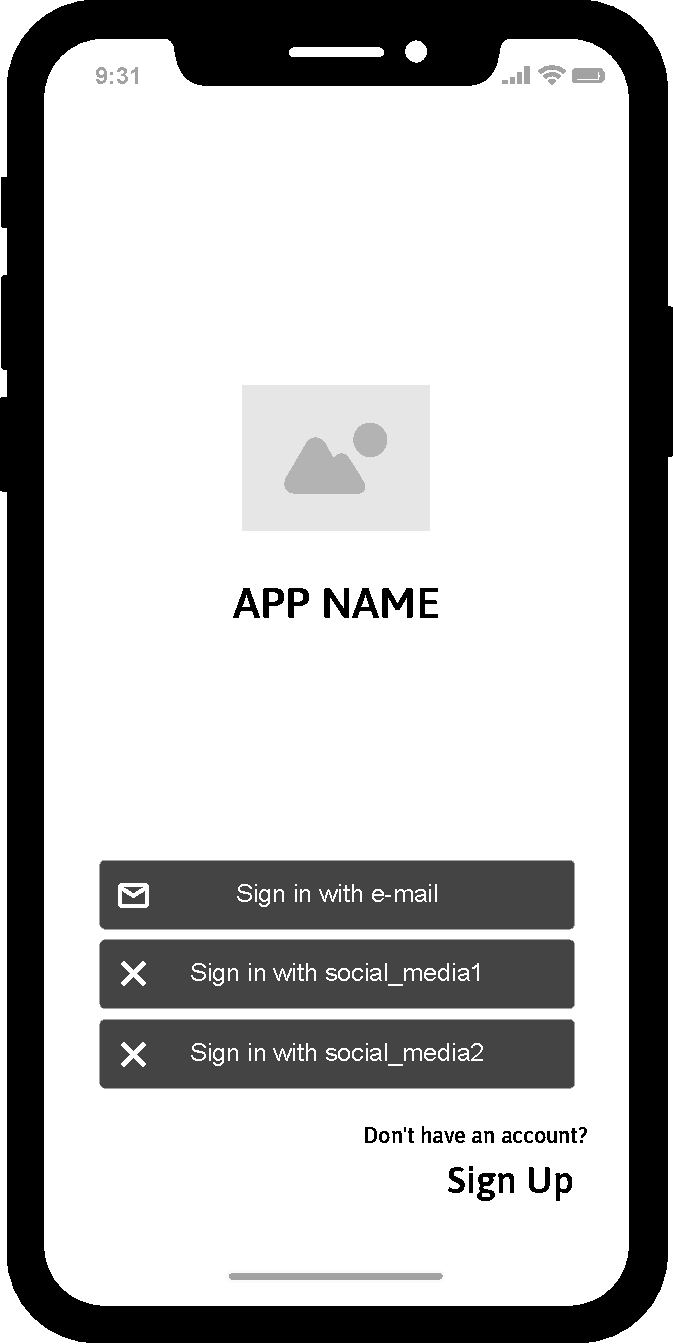
\includegraphics[width=0.4\textwidth]{Images/appScreens/signIn1.pdf}}\hfill
    \tmpframe{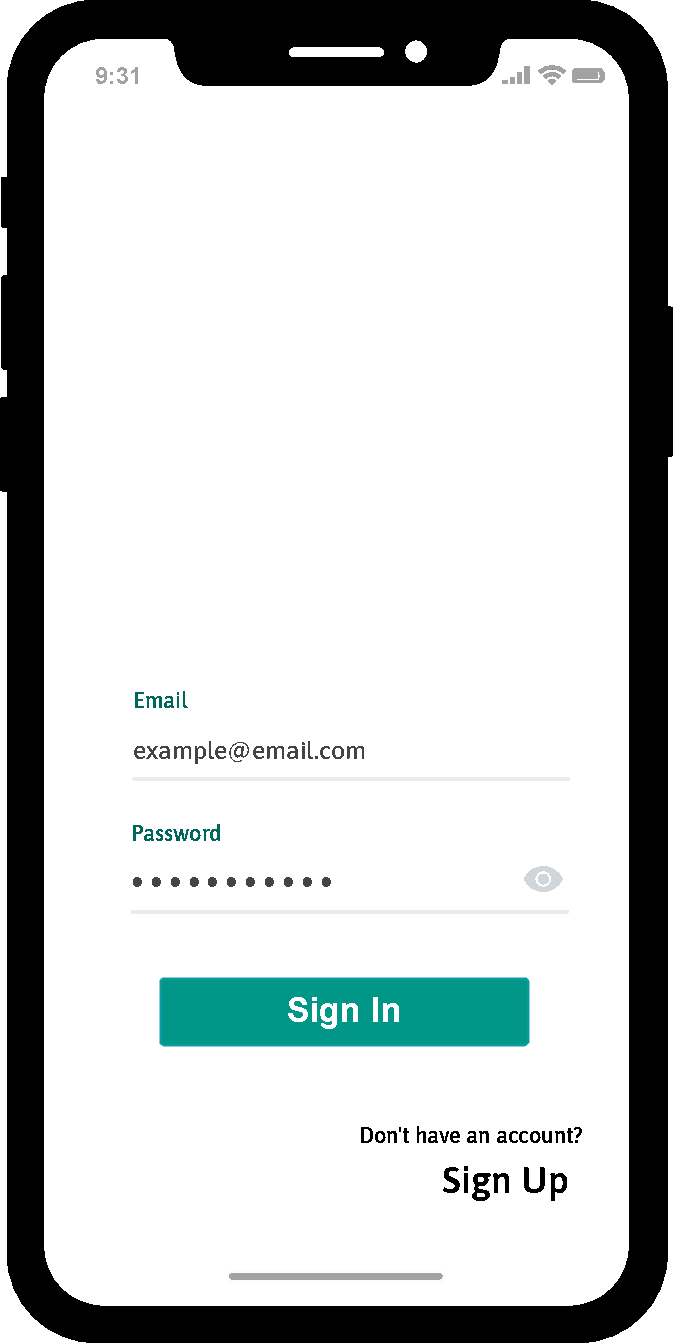
\includegraphics[width=0.4\textwidth]{Images/appScreens/signIn2.pdf}}
    \caption{Welcome screen with sign-in options and e-mail sign-in screen}
    \label{fig:sign-in-email}
\end{figure}

After signing up and creating a new account, there is a sequence of screens asking for the user's personal data, such as height, weight, biological sex, birth date, and whether they know about a condition that means their heart rate should be limited, and if so, how much (on a scale of 1 to 5).
Another screen asks the user to pair a watch with the APP, showing a list of Bluetooth devices paired with the phone.
The last one asks the user to take a fitness test, so that their fitness can be assessed.
This step can be skipped, but there's a warning about the inaccuracy of methods based on readily available data compared to taking a fitness test.
At the same time, the user is assured that the test can be taken later.

If the user decides to take the test, they are rerouted to the screen with fitness tests (without the bottom navigation bar).
Again, it is possible to quit this screen.

\section{Profile tab}
After setup, the APP opens on the `Profile' tab, displaying all entered and calculated information on cards, as well as the option to log out, and the currently active device~(fig.\ref{fig:profile1}).

\begin{figure}[h!]
    \centering
    \tmpframe{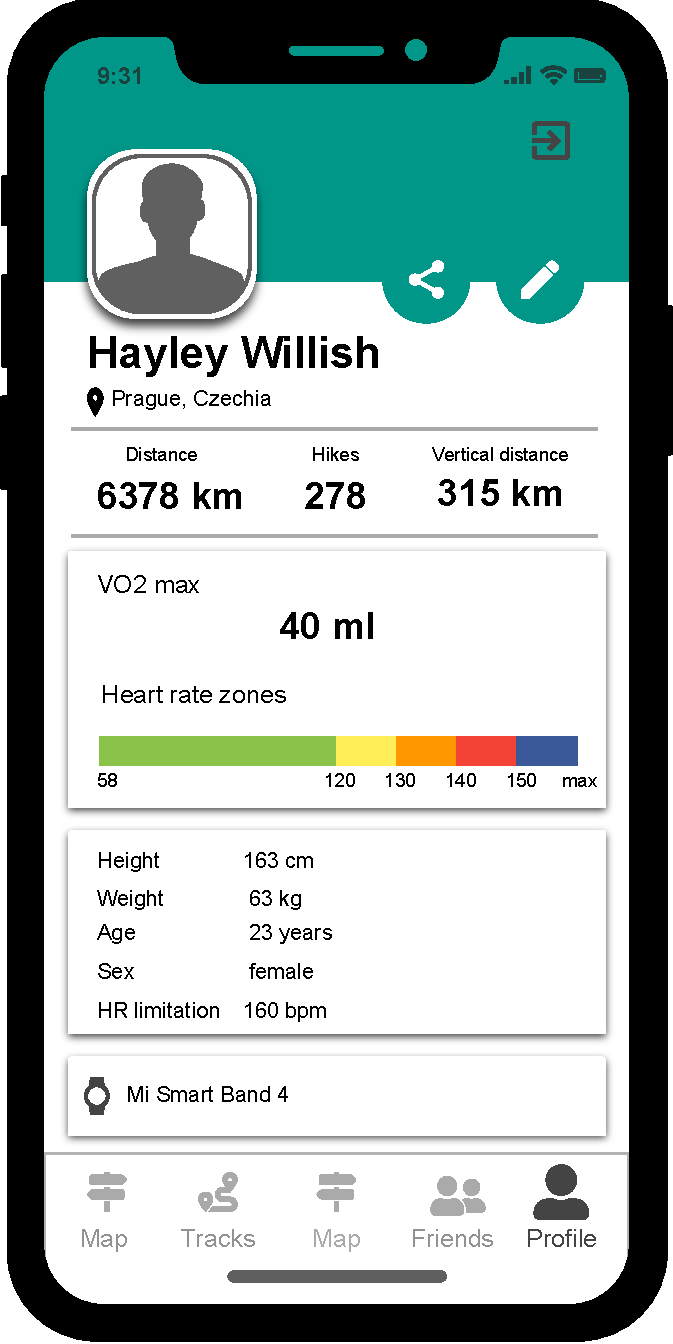
\includegraphics[width=0.4\textwidth]{Images/appScreens/profile1.pdf}}\hfill
    \caption{The Profile screen}
    \label{fig:profile1}
\end{figure}

The card with fitness opens to show the user's fitness data -- VO2 max, heart rate zones, and minimum and maximum heart rate.
The heart rate zones are color-coded; these colors occur in the whole application to signify difficulty.
There's an icon to get more information about the metrics (excerpts from the Fitness Assessment chapter), and the option to take a fitness test~(fig.\ref{fig:fitnessInfo}).
The pictures are placeholders for charts of development of the metric over time.

\begin{figure}[h!]
    \centering
    \tmpframe{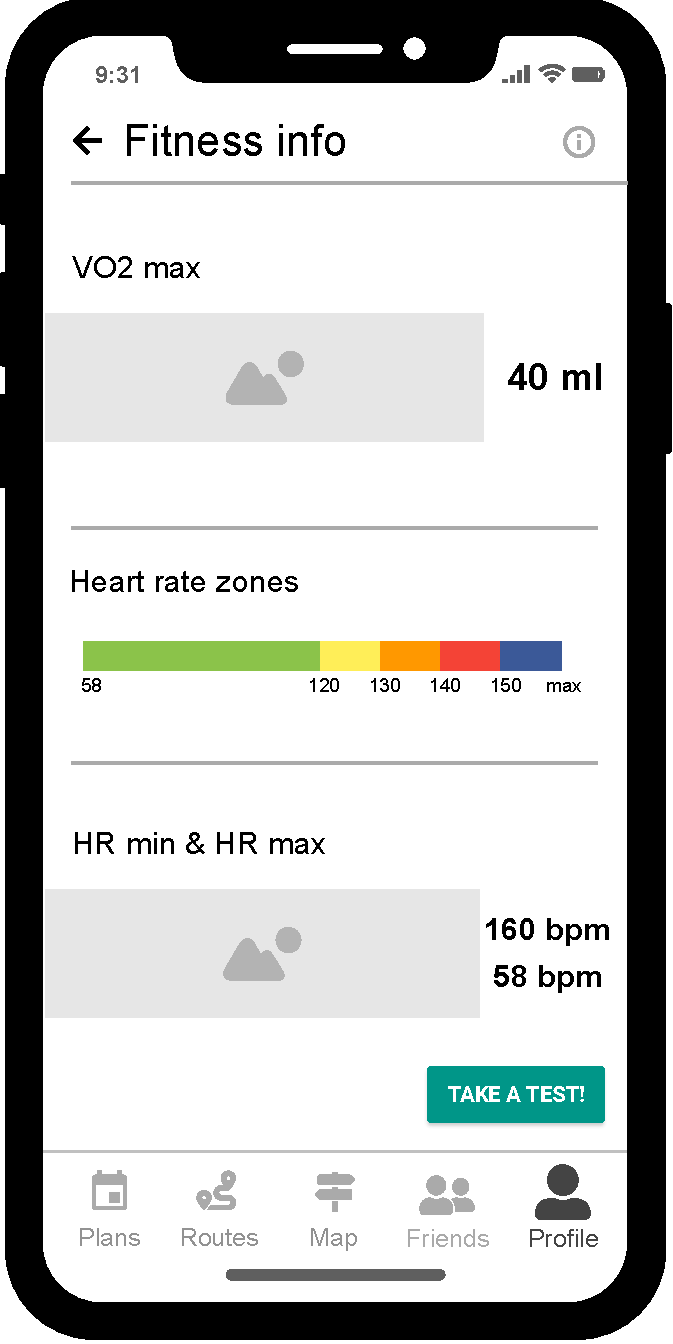
\includegraphics[width=0.4\textwidth]{Images/appScreens/profile-fitnessInfo.pdf}}\hfill
    \caption{Fitness information}
    \label{fig:fitnessInfo}
\end{figure}

On the `Fitness tests' screen, the user can choose between multiple tests, each of which has a tag saying what it tests~(fig.\ref{fig:fitnessTests}).
As an example, the `6 Minute Walking Test' screen has directions on what the user should do, and after the test, there is a screen with results~(fig.\ref{fig:6mwt}).
Again, the pictures will contain the charts of the metric's values over the course of the test.

\begin{figure}[h!]
    \centering
    \tmpframe{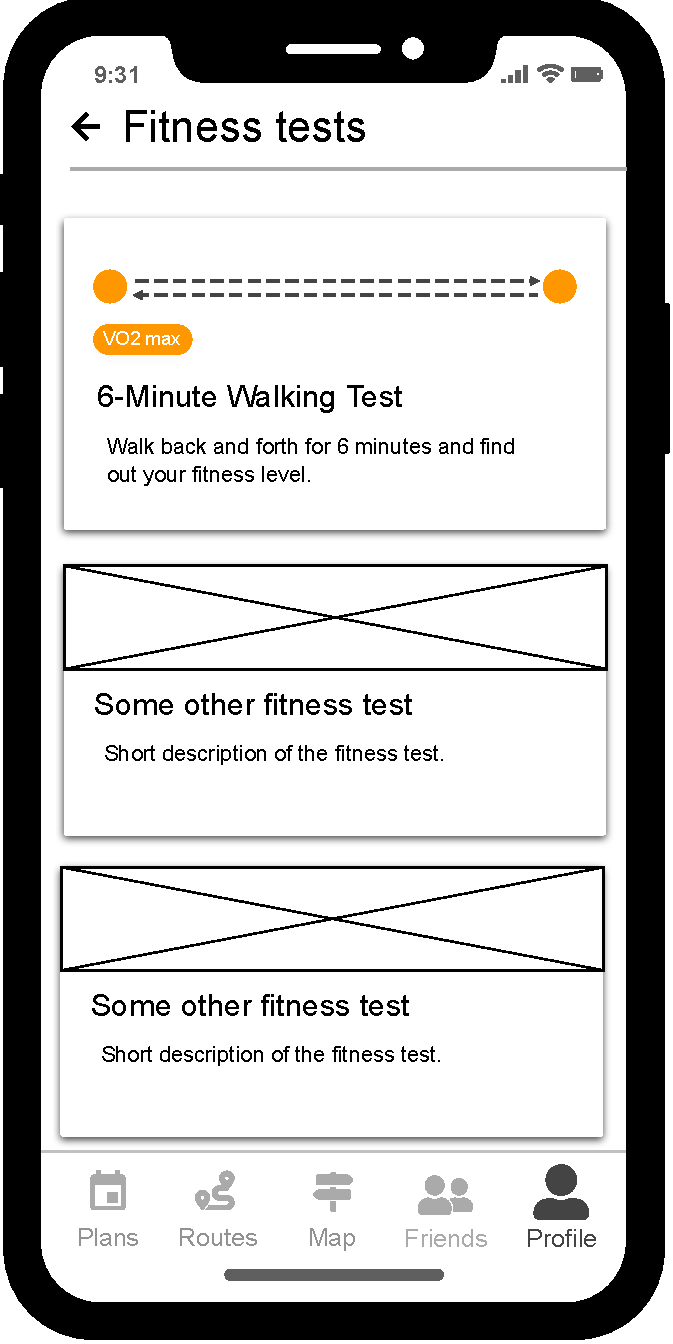
\includegraphics[width=0.4\textwidth]{Images/appScreens/profile-fitnessTests.pdf}}\hfill
    \caption{Fitness tests}
    \label{fig:fitnessTests}
\end{figure}

\begin{figure}[h!]
    \centering
    \tmpframe{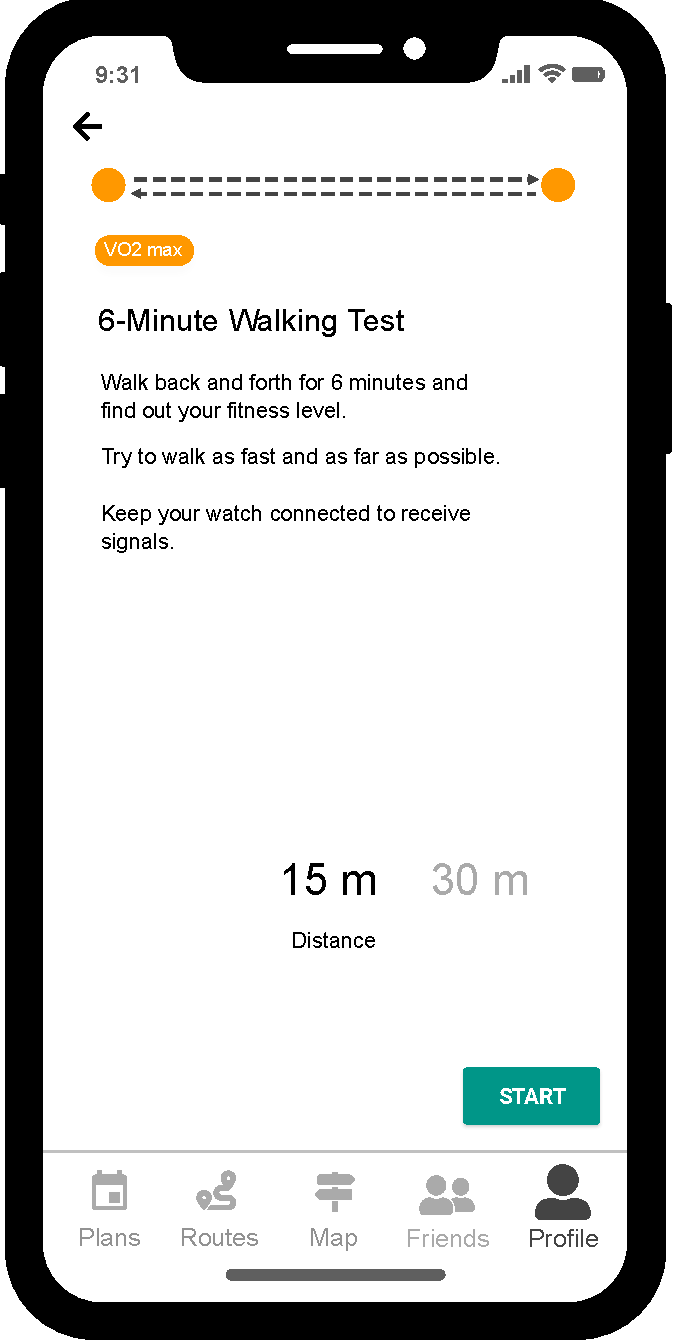
\includegraphics[width=0.4\textwidth]{Images/appScreens/profile-fitness-6mwt.pdf}}\hfill
    \tmpframe{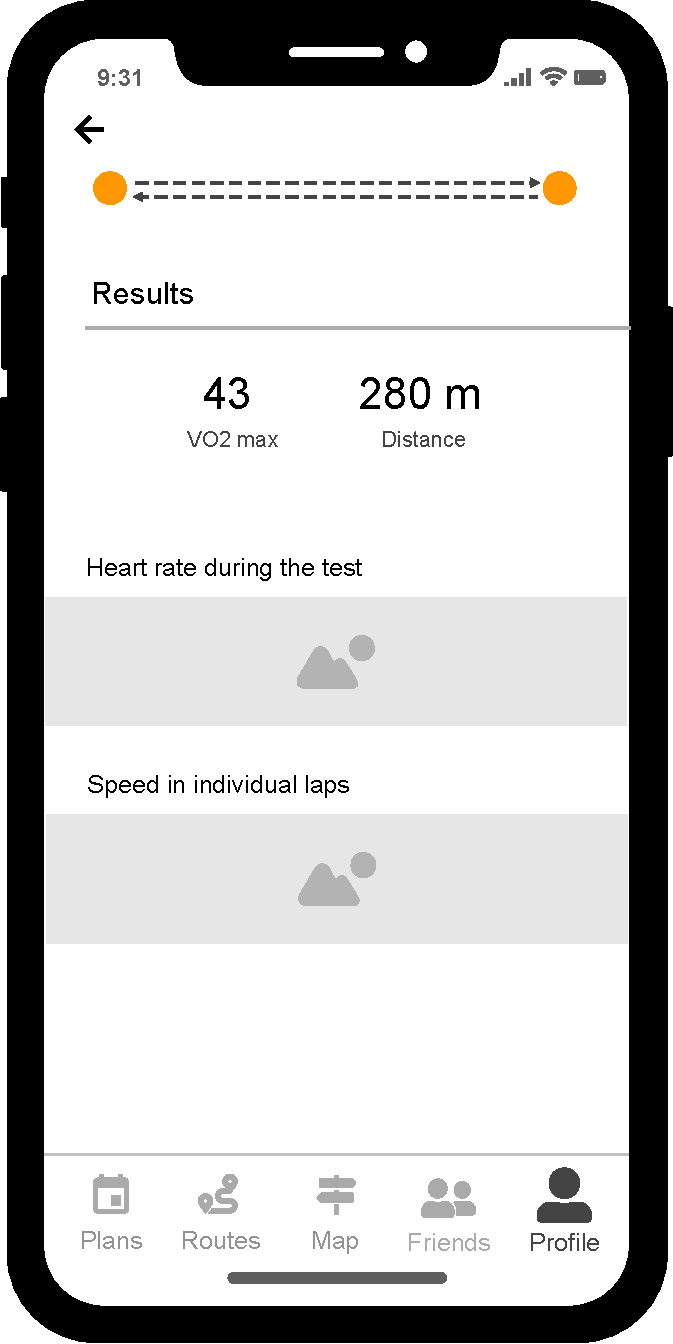
\includegraphics[width=0.4\textwidth]{Images/appScreens/profile-fitness-6mwt-results.pdf}}
    \caption{6 Minute Walking Test}
    \label{fig:6mwt}
\end{figure}

When we come back to the `Profile' screen (fig.\ref{fig:profile1}), we can also manually edit all the information the user has provided.
The profile picture, basic data like height etc., as well as the fitness information.

Another option from here is to see the devices by expanding the card with the active device.
The `Devices' screen~(fig.\ref{fig:devices}) contains the active device which can be deactivated, as well as other paired devices, which can be either activated or unpaired.
The user can also pair a new device with the app (opening a list of devices paired with the phone).
Tapping the `Activate' button will deactivate the currently active device.

\begin{figure}[h!]
    \centering
    \tmpframe{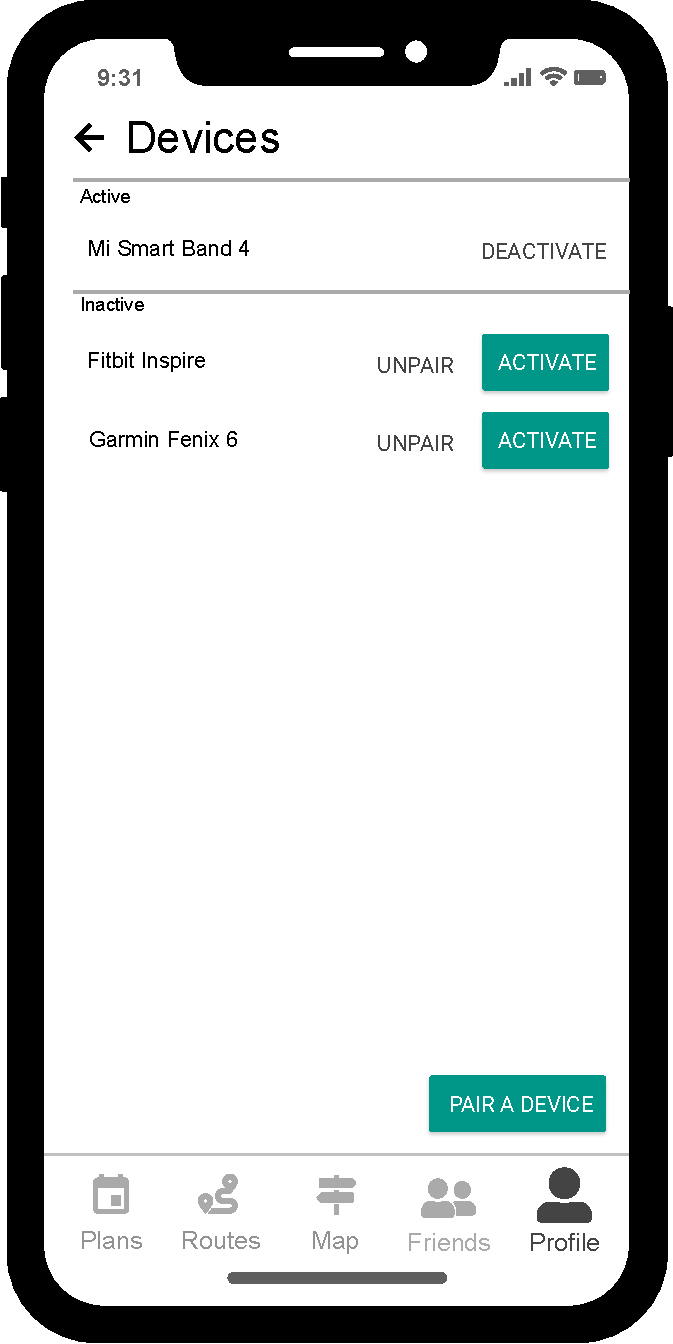
\includegraphics[width=0.4\textwidth]{Images/appScreens/profile-devices.pdf}}\hfill
    \caption{Devices}
    \label{fig:devices}
\end{figure}

\section{Map tab}
The default tab on which the application opens is the `Map' tab~(fig.\ref{fig:map}).
This is where the user can look at the integrated map, as well as search for specific places~(fig.\ref{fig:map-searchPlace}) and add them as waypoints to the planned route.
The waypoint will be added to the route as the `next' waypoint.

\begin{figure}[h!]
    \centering
    \tmpframe{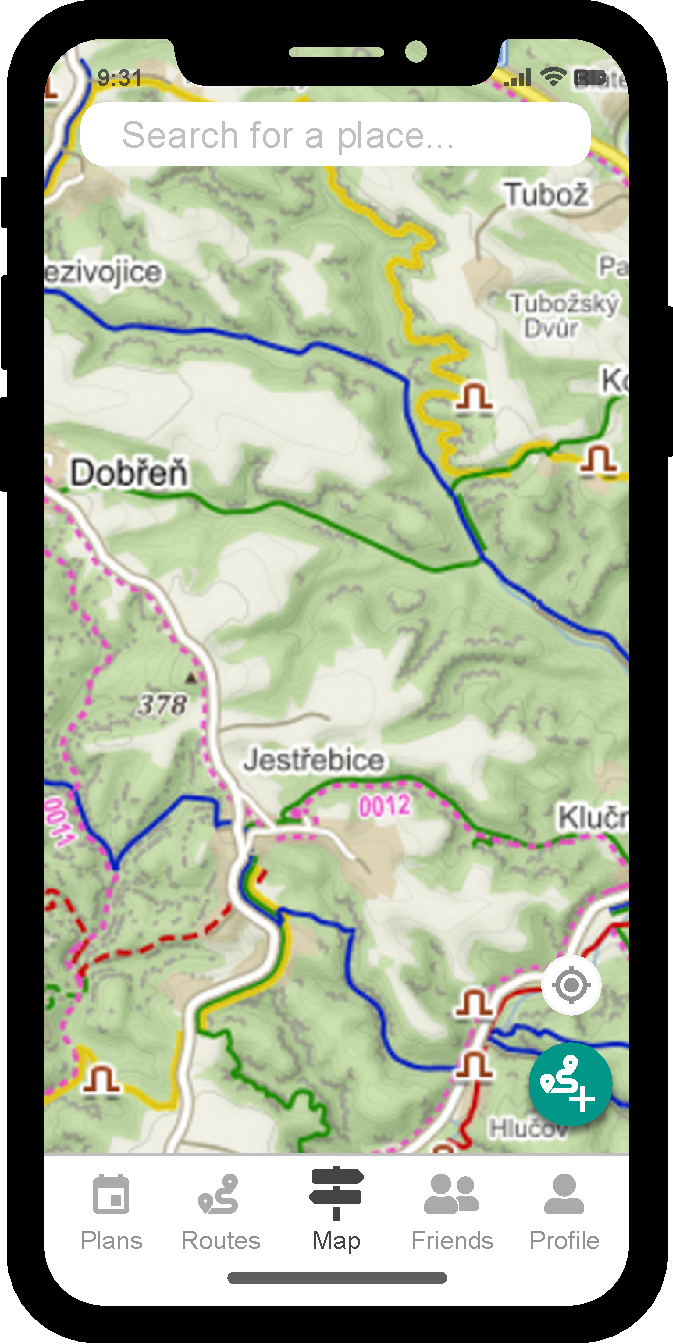
\includegraphics[width=0.4\textwidth]{Images/appScreens/maps1.pdf}}\hfill
    \caption{Map screen}
    \label{fig:map}
\end{figure}

\begin{figure}[h!]
    \centering
    \tmpframe{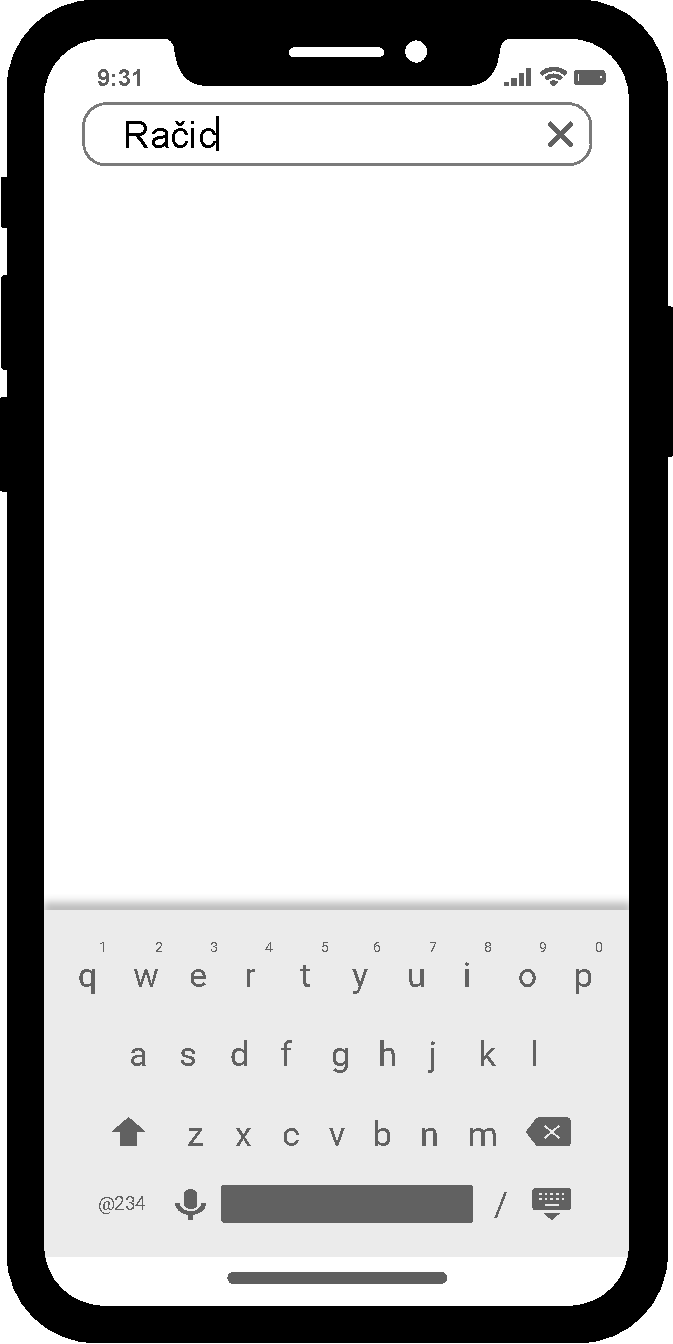
\includegraphics[width=0.3\textwidth]{Images/appScreens/map-search1.pdf}}\hfill
    \tmpframe{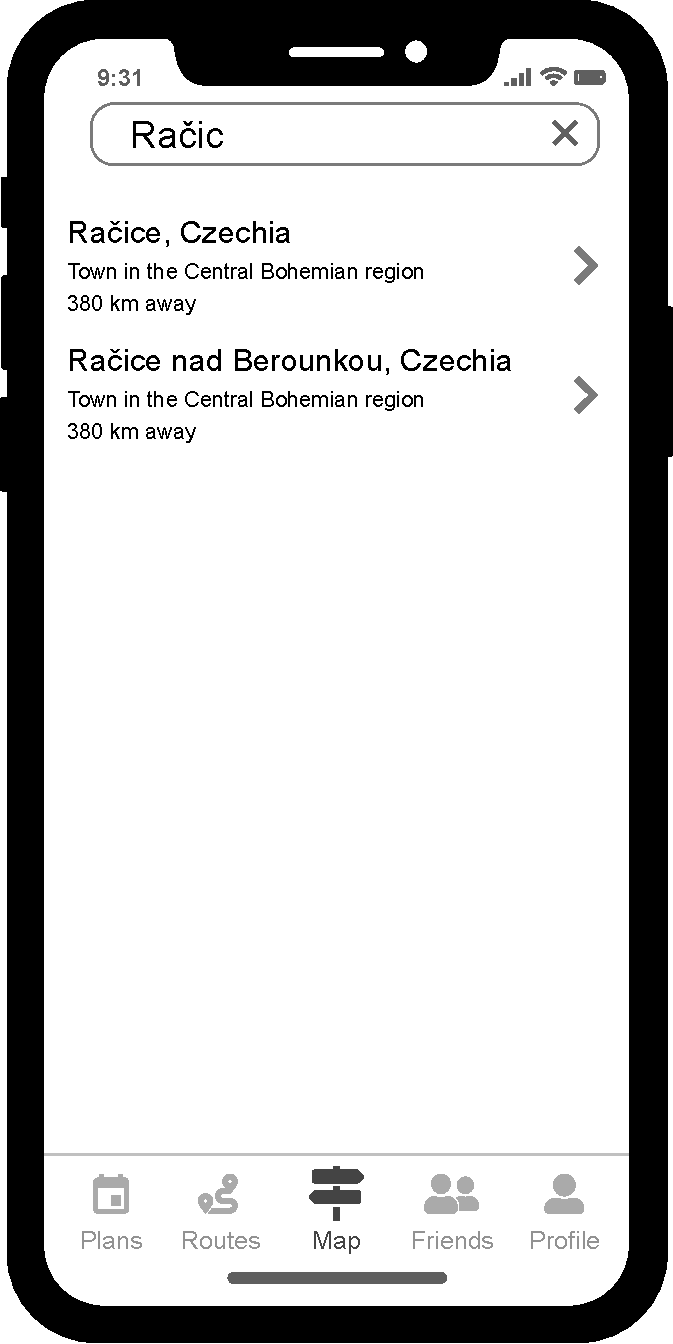
\includegraphics[width=0.3\textwidth]{Images/appScreens/map-search2.pdf}}\hfill
    \tmpframe{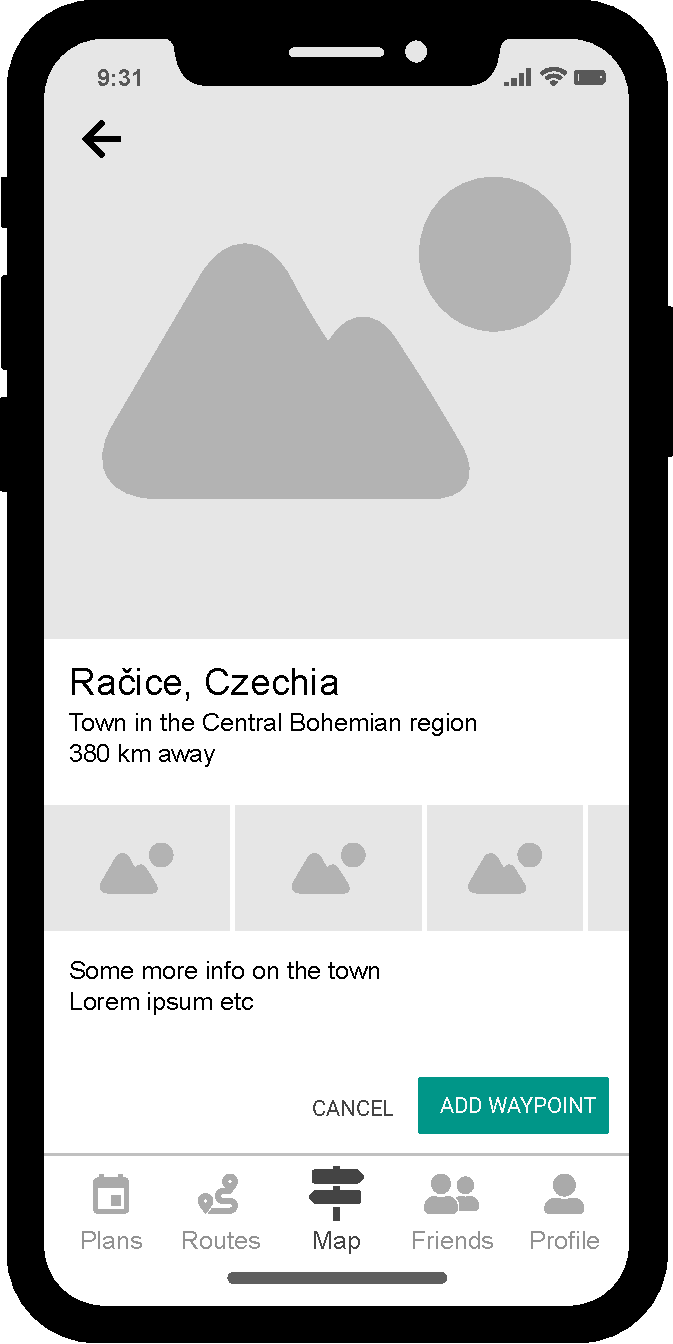
\includegraphics[width=0.3\textwidth]{Images/appScreens/map-search3.pdf}}\hfill
    \caption{Search for a place}
    \label{fig:map-searchPlace}
\end{figure}

Planning a new route can also be started with the floating button on the bottom right of the screen~(fig.\ref{fig:map}).

The planning process consists of three steps:
\begin{enumerate}
    \item waypoints,
    \item pick a route, and
    \item plan a hike.
\end{enumerate}

In the `Waypoints' step~fig.\ref{fig:plan-waypoints}), the user picks where they want to start their route, the destination, and all the points through which they want to pass.
Each of the points can be picked directly from the map with a long press, or by searching for a place~(fig.\ref{fig:map-searchPlace}).
The current location can also be used as a starting point.
The intermediate points can be added using the plus button, and all the waypoints can be rearranged by drag'n'dropping each line by the menu icon on the left.
The user can also remove individual waypoints using the X icon on the right: when removing the starting or destination point, only the text is removed, since every route needs two points.

Another option is to choose a return trip, where the platform should offer routes that start in the starting point, go through the destination, and either give a different route to go back if possible, or has the user retrace their steps.

\begin{figure}[h!]
    \centering
    \tmpframe{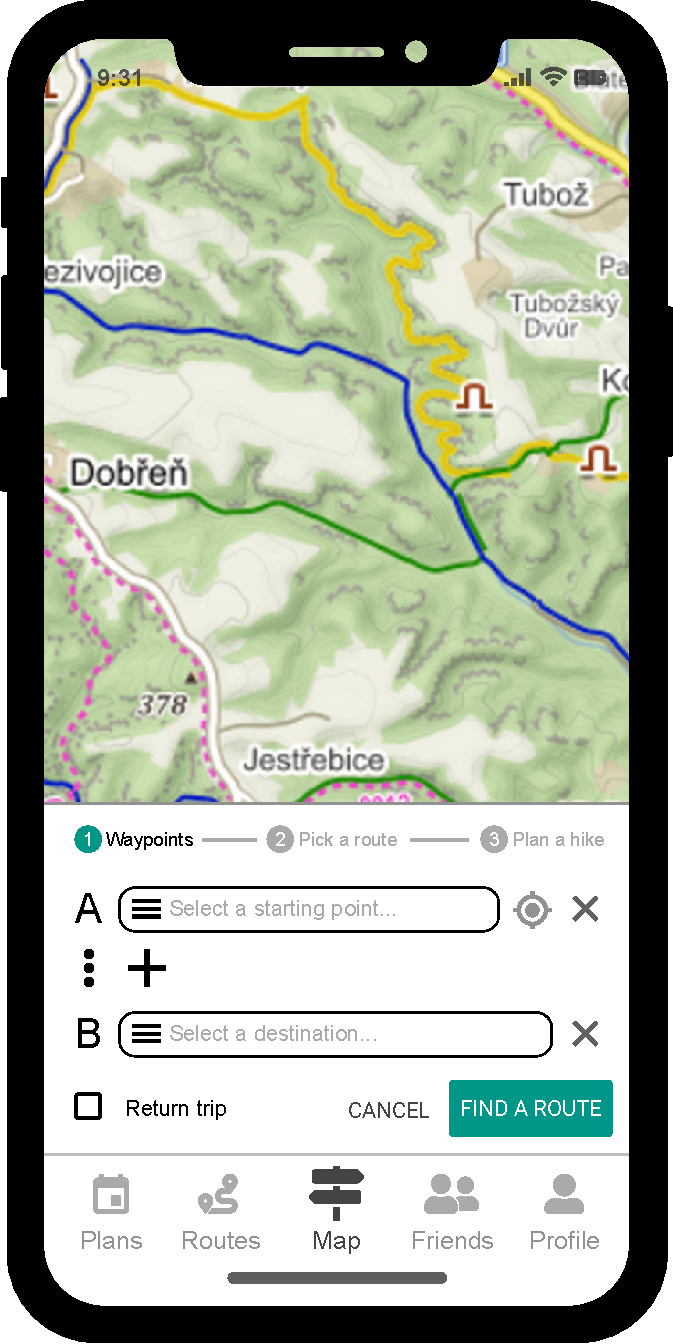
\includegraphics[width=0.4\textwidth]{Images/appScreens/map-plan1.pdf}}\hfill
    \tmpframe{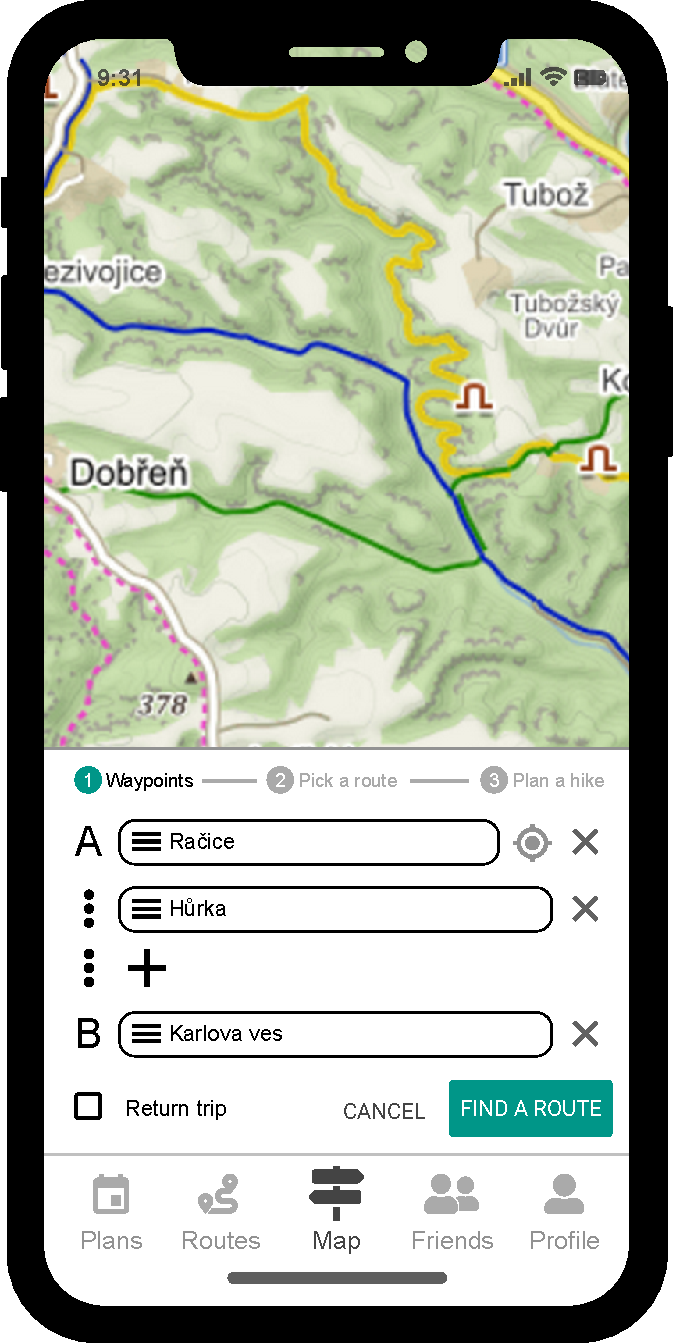
\includegraphics[width=0.4\textwidth]{Images/appScreens/map-plan2.pdf}}\hfill
    \caption{Planning a route with waypoints}
    \label{fig:plan-waypoints}
\end{figure}

When the user is satisfied with the waypoints, they tap the `Find a route' button.
In this step the planning UI pulls up higher, covering a larger part of the map, while the visible part of the map contains all the route options on an appropriately zoomed-in map.
The chosen option is highlighted, while the others are less opaque.
The options can be switched between by tapping on the map.

The middle of the planning UI now contains the details of the chosen route -- the time it will get the user to hike it if they go alone, its elevation, length, prevalent surface type, and a difficulty chart.

The bottom part of the planning UI has information on individual segments of the route.
The picture is a placeholder for the route's elevation profile, which has two interactive sliders to pick the segment whose details the user wants to know.
These details include its elevation, surface, and a difficulty chart.

The route can be saved and unsaved by tapping the bookmark icon, and shared via link by tapping the share icon.

If the user wants to just start the hike without planning for a different day or inviting friends, they can press the `GO' button and the APP navigates him,
or they can continue to the next step: Plan a hike.

\begin{figure}[h!]
    \centering
    \tmpframe{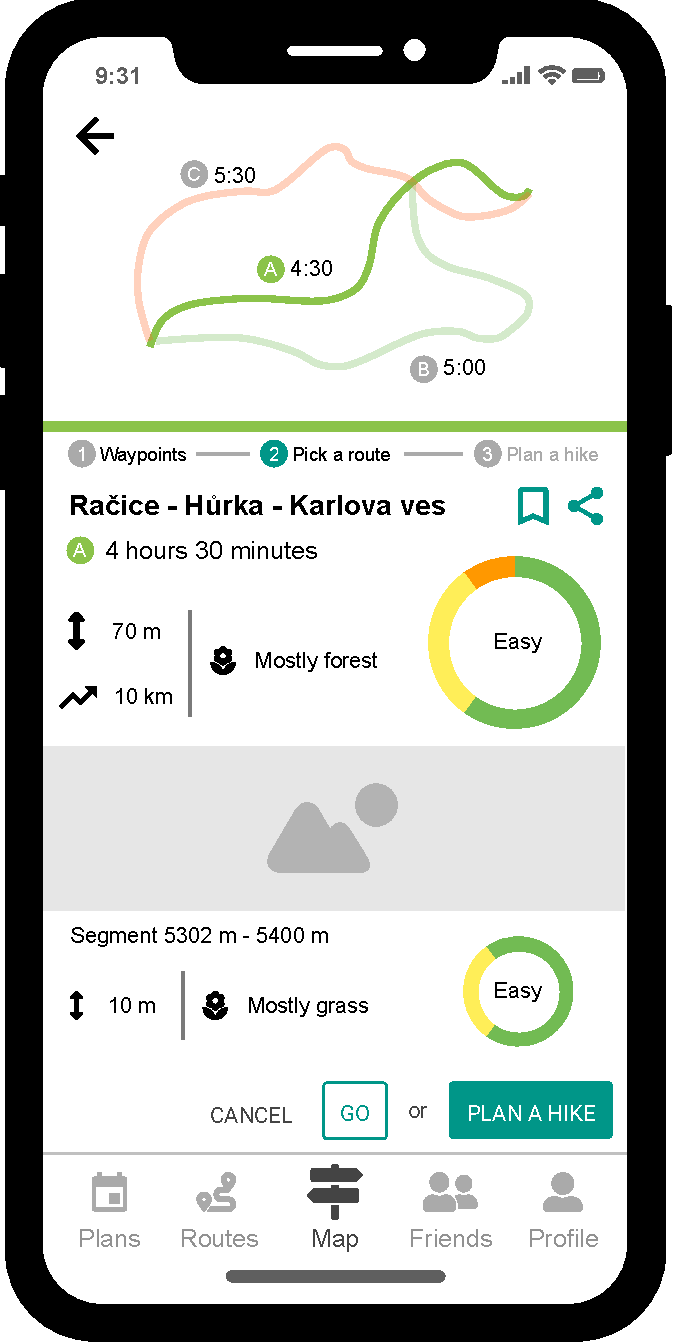
\includegraphics[width=0.4\textwidth]{Images/appScreens/map-plan3.pdf}}\hfill
    \tmpframe{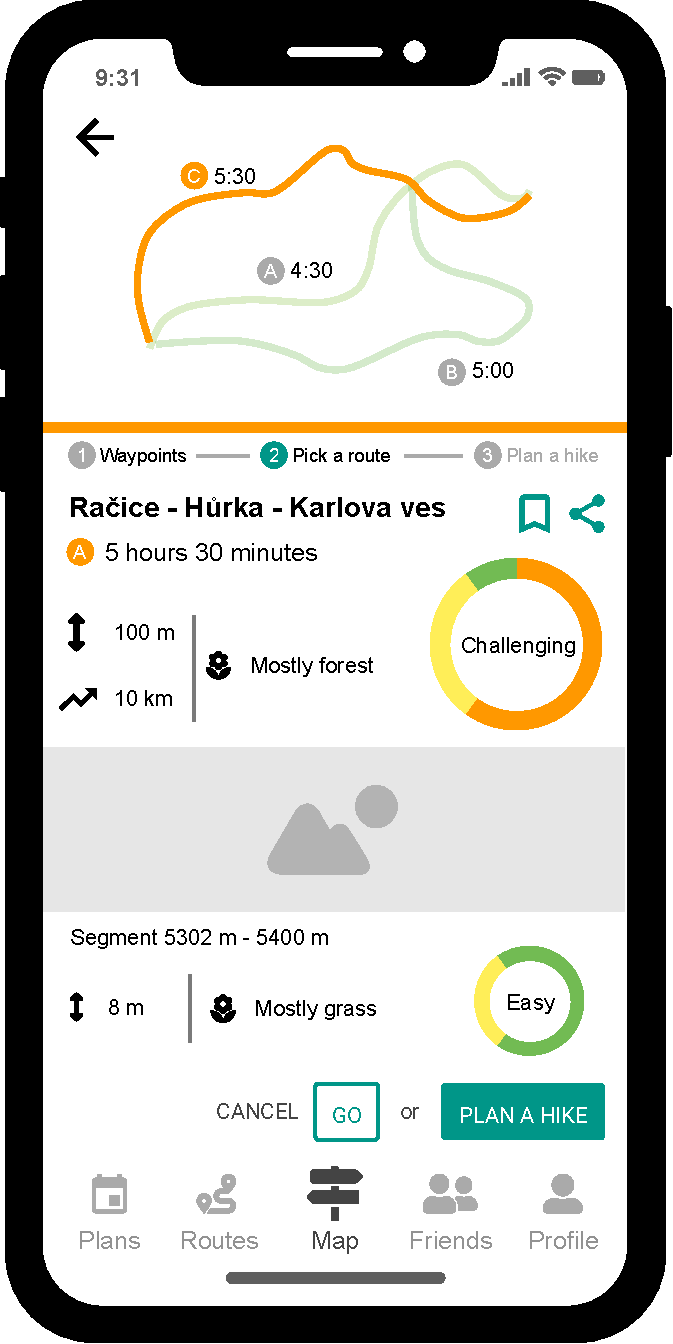
\includegraphics[width=0.4\textwidth]{Images/appScreens/map-plan4.pdf}}\hfill
    \caption{Picking a route based on its details.}
    \label{fig:plan-pick-route}
\end{figure}

The last step is planning a hike.
This means choosing the date with a date picker, and the people to join the user~(fig.\ref{fig:plan-plan-hike}).
These can be searched for among the user's friends, using the `invite people' button~(fig.\ref{fig:plan-invite-friends}).
While searching for friends, their avatars are added to the summary on the bottom and the counter is incremented.

\begin{figure}[h!]
    \centering
    \tmpframe{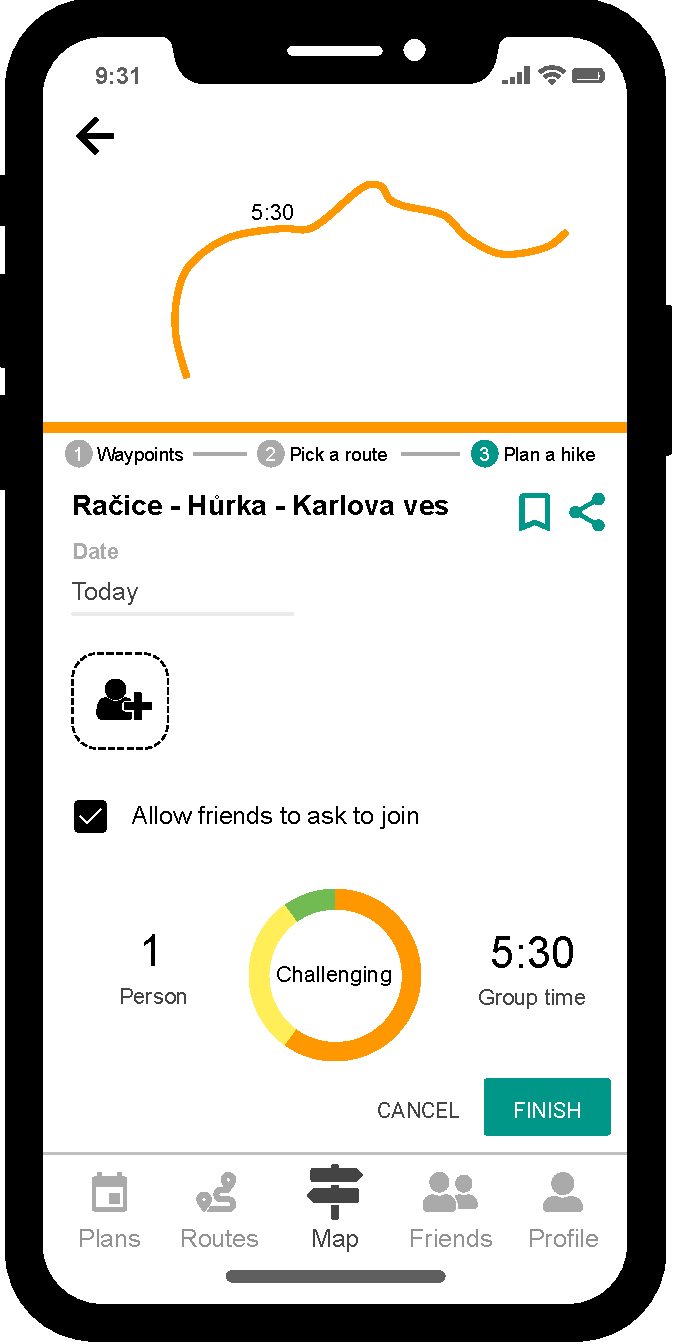
\includegraphics[width=0.4\textwidth]{Images/appScreens/map-plan5.pdf}}\hfill
    \caption{The initial state of a planned hike.}
    \label{fig:plan-plan-hike}
\end{figure}

\begin{figure}[h!]
    \centering
    \tmpframe{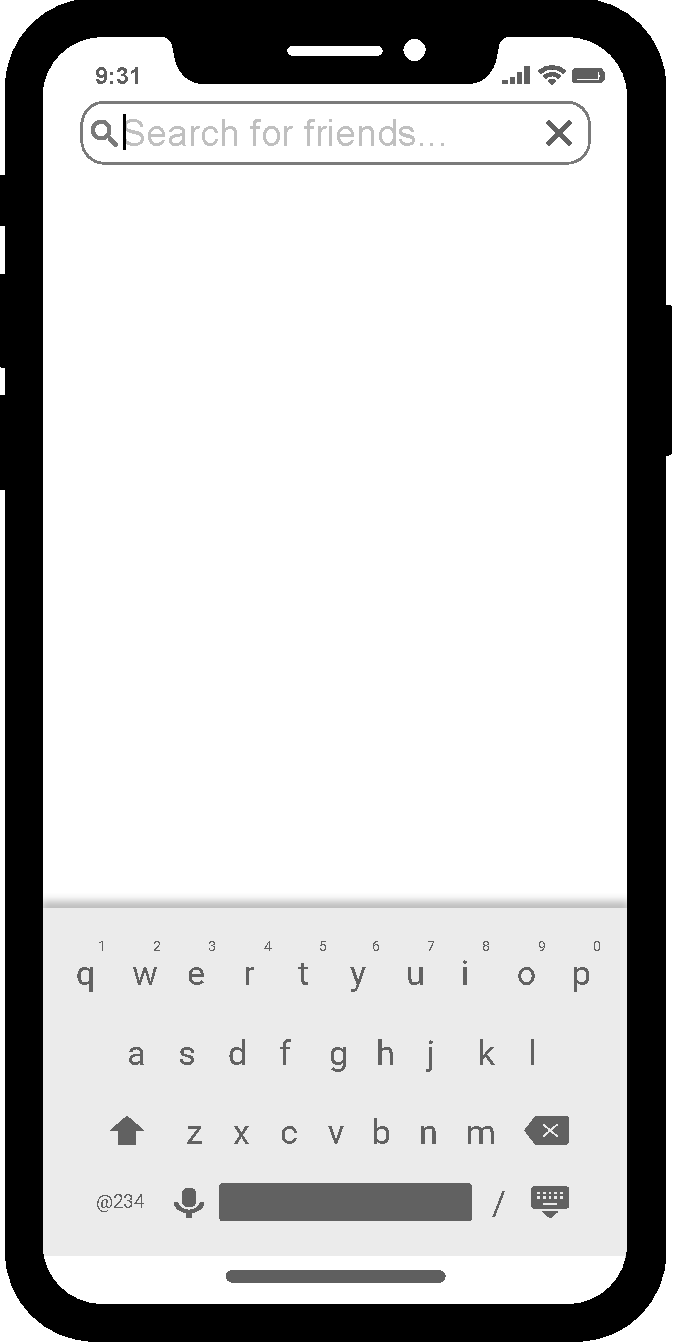
\includegraphics[width=0.4\textwidth]{Images/appScreens/map-plan6-friends.pdf}}\hfill
    \tmpframe{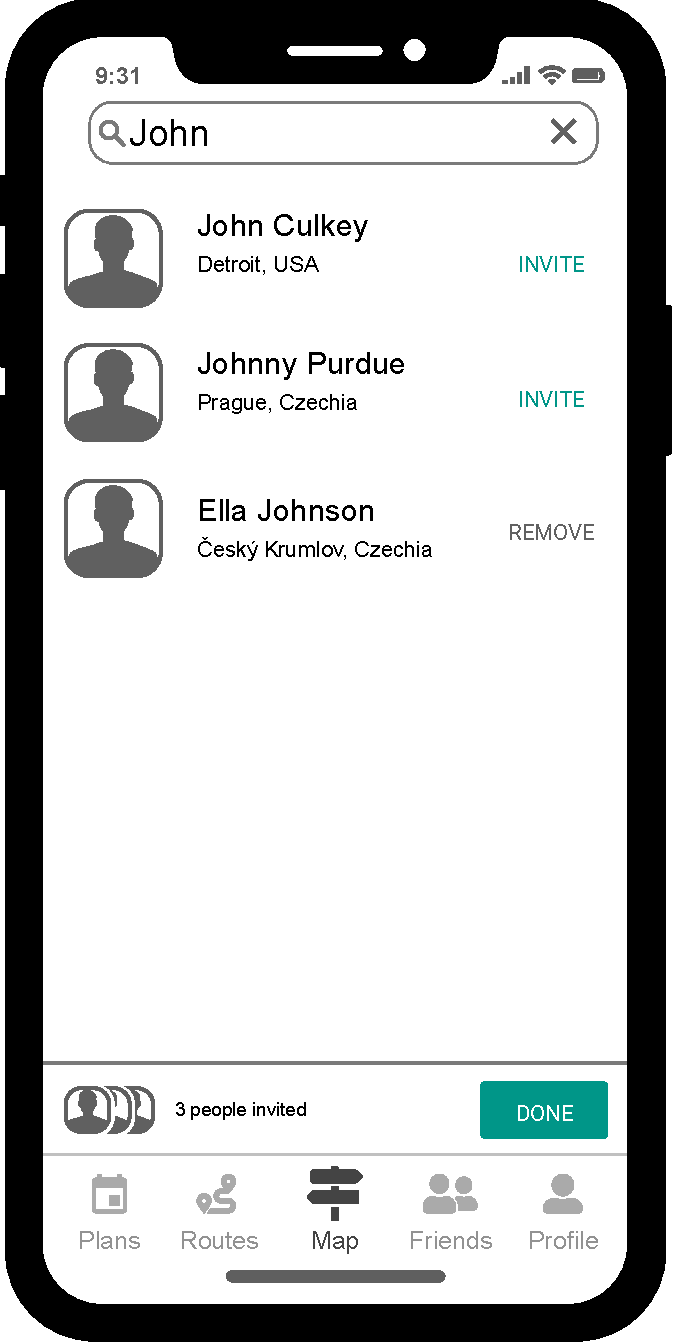
\includegraphics[width=0.4\textwidth]{Images/appScreens/map-plan7-friends.pdf}}\hfill
    \caption{Searching for friends to invite to a hike. A summary of already chosen people is on the bottom.}
    \label{fig:plan-invite-friends}
\end{figure}

Once the friends are chosen, the user can see a summary of the hike, with the difficulty chart adjusted to the group's common fitness (fig.\ref{fig:plan-end}), the number of people who are coming or invited, and how long it is going to take them.

This screen also contains a checkbox to allow friends join the hike -- whether the hike should be marked as joinable when it is shared to the friends' feed of `All plans'~(fig.\ref{fig:plan-all-plans}).

Once the planning is finished, we return to the basic `Map' screen, with a snack bar notification telling the user where they can find the planned hike and how many people were invited~(fig.\ref{fig:plan-end}).

The whole planning can be stopped at any point with the `Cancel' button, which will trigger a confirmation dialogue, as the user is about to delete all their progress, and after confirming, we return to the `Map' tab.

\begin{figure}[h!]
    \centering
    \tmpframe{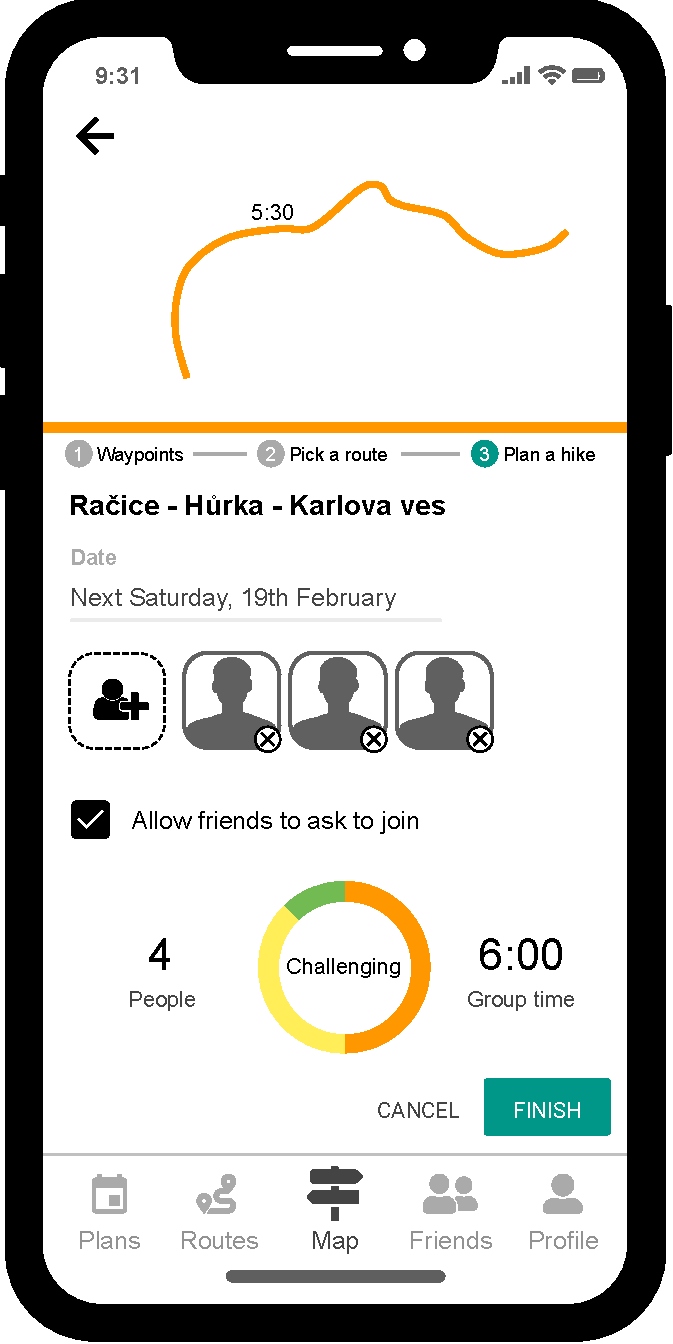
\includegraphics[width=0.4\textwidth]{Images/appScreens/map-plan8.pdf}}\hfill
    \tmpframe{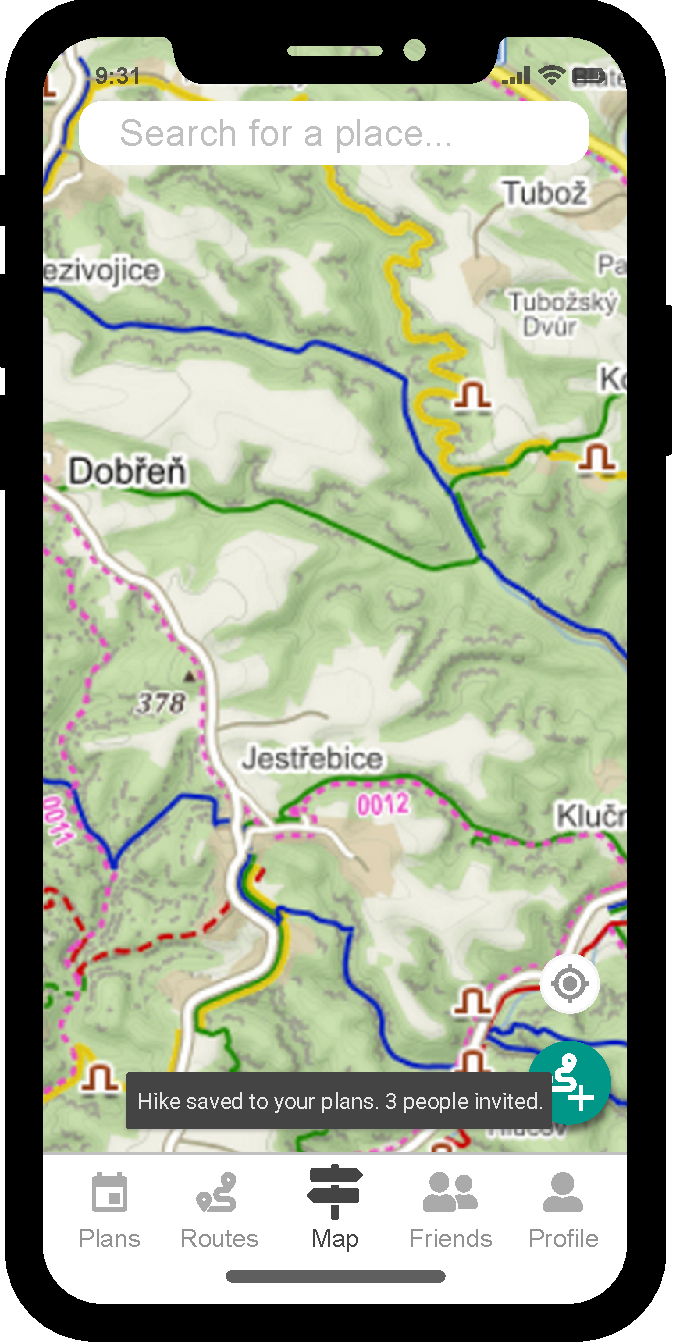
\includegraphics[width=0.4\textwidth]{Images/appScreens/map-plan9.pdf}}\hfill
    \caption{Overview of the hike. After pressing the `Finish' button, we are back to the `Map' screen.}
    \label{fig:plan-end}
\end{figure}

\section{Plans tab}
The `Plans' tab is divided into three sections -- `All plans', `My plans' and `History'.
The default `All plans' section~(fig.\ref{fig:plan-all-plans}) is a filterable feed of the users' and their friends' upcoming plans.
This is also where the user's invitations to friends' hikes are displayed; these can be either dismissed or accepted.

A collapsed hike card contains basic information, the route on a map (represented by the picture placeholder) such as who hosts it, when it is happening and how long it will take, whether it is joinable and how difficult it would be for the user.

When tapping on the card, the card expands to show more of the hike's details: 
who is coming, how long it is currently planned to be plus how much longer it will take if the user joins, and all of its information recalculated to the user's fitness.

If the hike is joinable, there is an `Ask to join' button; if not, the user can only go back.

Again, there are the options to save the route, and share either the route or the hike, which is chosen in a dropdown dialogue.

\begin{figure}[h!]
    \centering
    \tmpframe{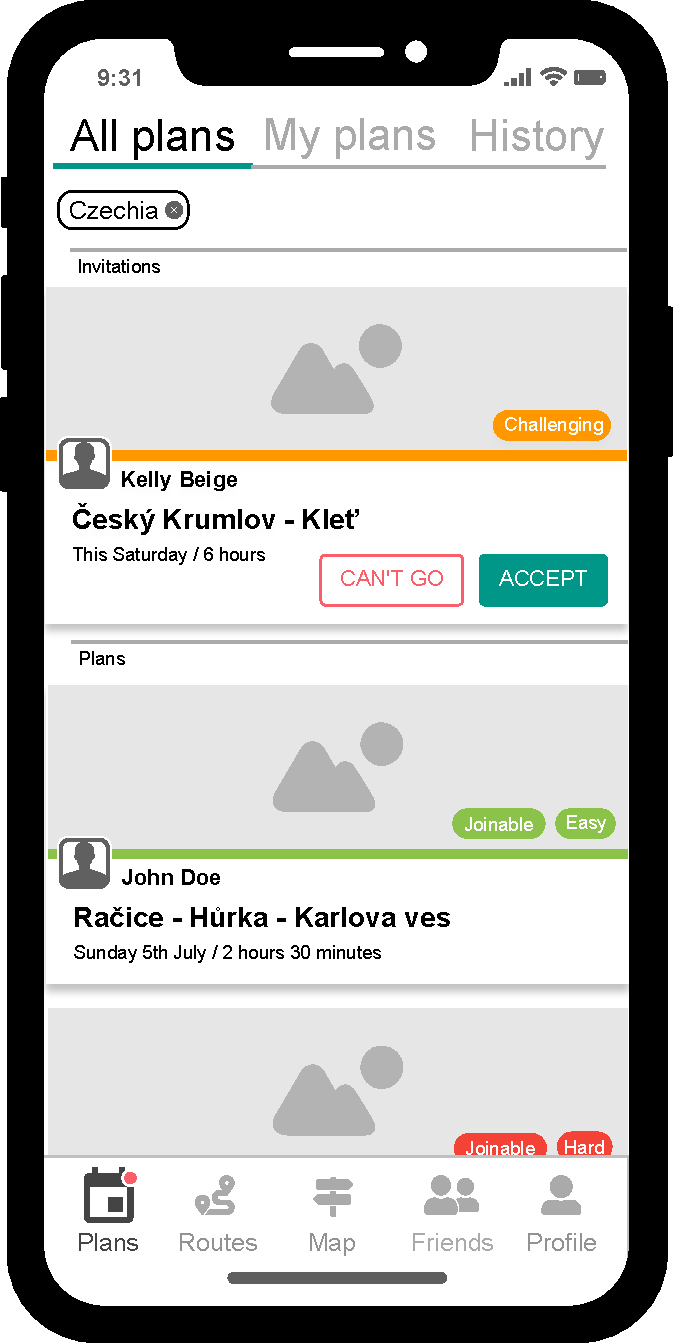
\includegraphics[width=0.4\textwidth]{Images/appScreens/plans-all-plans.pdf}}\hfill
    \tmpframe{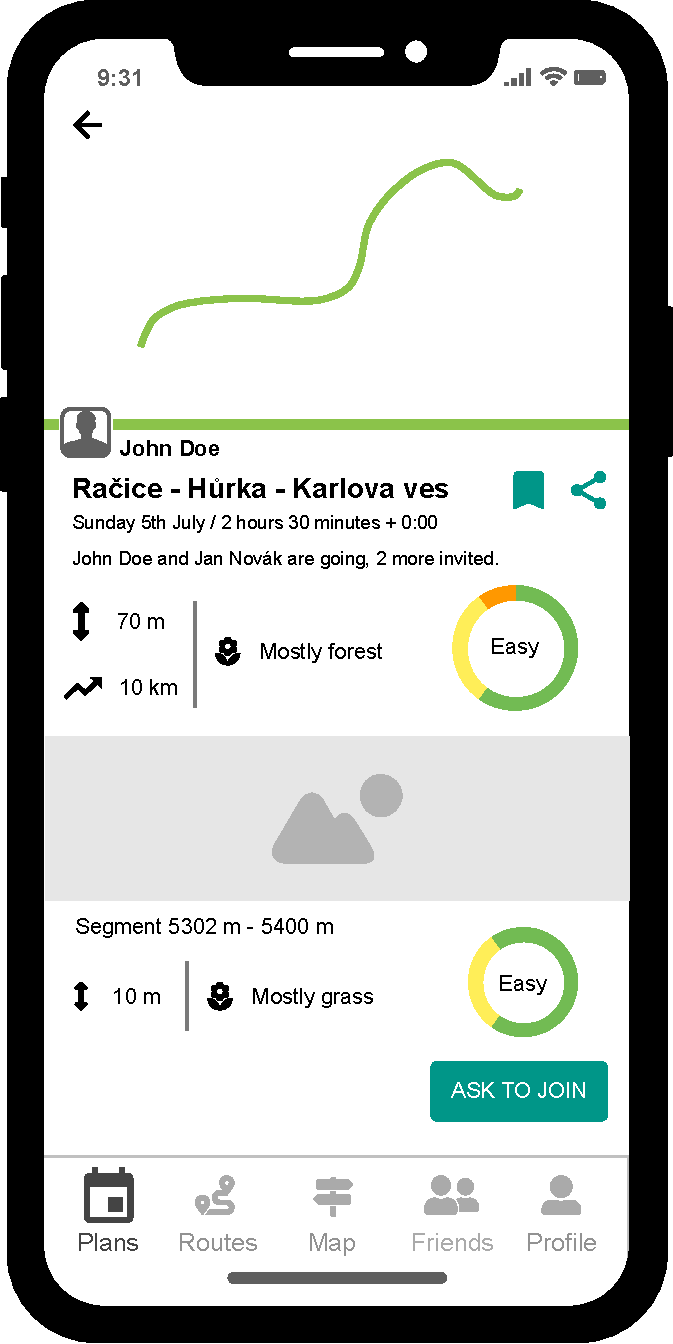
\includegraphics[width=0.4\textwidth]{Images/appScreens/plans-all-plans-joinable-detail.pdf}}\hfill
    \caption{All plans feed. Detail of a joinable hike.}
    \label{fig:plan-all-plans}
\end{figure}

The `My plans' section~(fig.\ref{fig:plan-my-plans}) contains the hikes that the user has planned or joined.
The detail of a hike planned by the user is different, compared to looking at hikes planned by other people,
since there have to be options to administer the hike.
Requests to join are shown in this detail; by tapping at the `People' section the user can manage the people connected to the hike, as well as allow or disallow people to join the hike.
The route can be cancelled by the red trash icon, and the user can also let others know that they can't go.
If the user is the host of the hike, they have to appoint a new host from the people who have accepted the invitation.

The `Start' button will become active on the day of the hike.
When it is pressed, the route will be activated on the phones of all the attendants, allowing to switch to navigation mode.

Tapping on the `Route' section will show the route's details, just like in fig.\ref{fig:plan-pick-route}.

\begin{figure}[h!]
    \centering
    \tmpframe{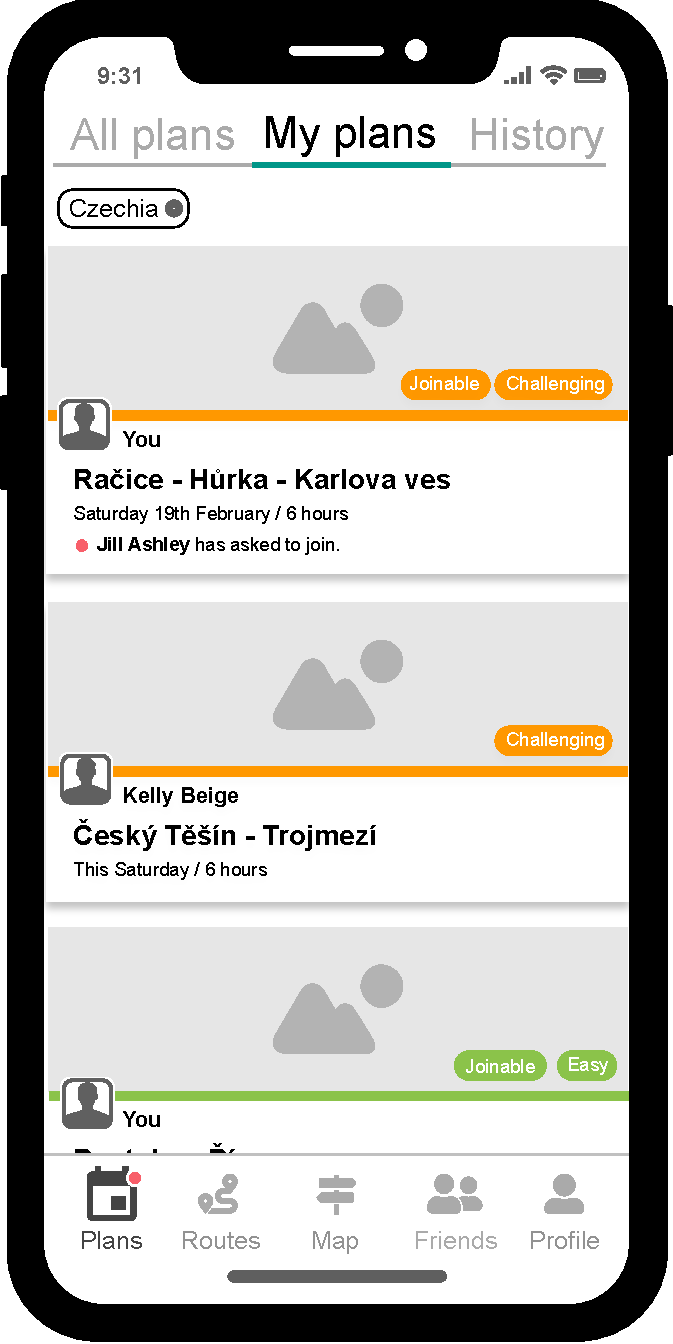
\includegraphics[width=0.3\textwidth]{Images/appScreens/plans-my-plans.pdf}}\hfill
    \tmpframe{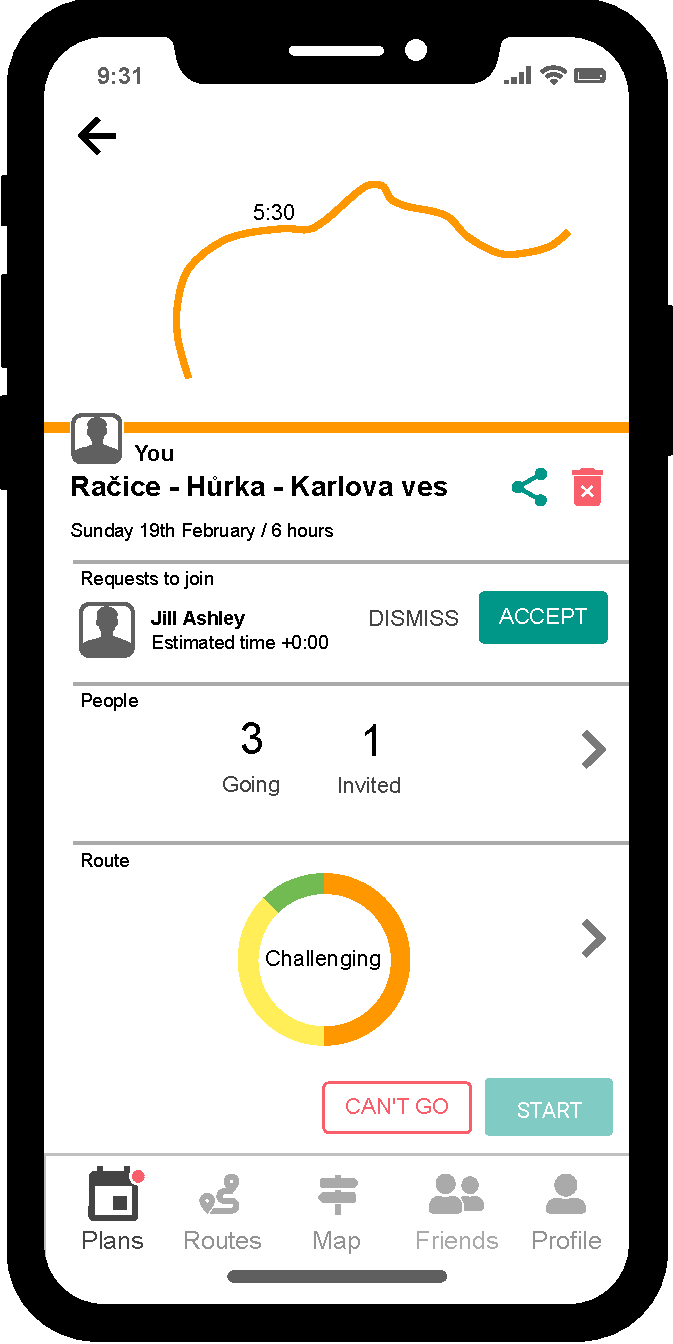
\includegraphics[width=0.3\textwidth]{Images/appScreens/plans-my-plans-detail.pdf}}\hfill
    \tmpframe{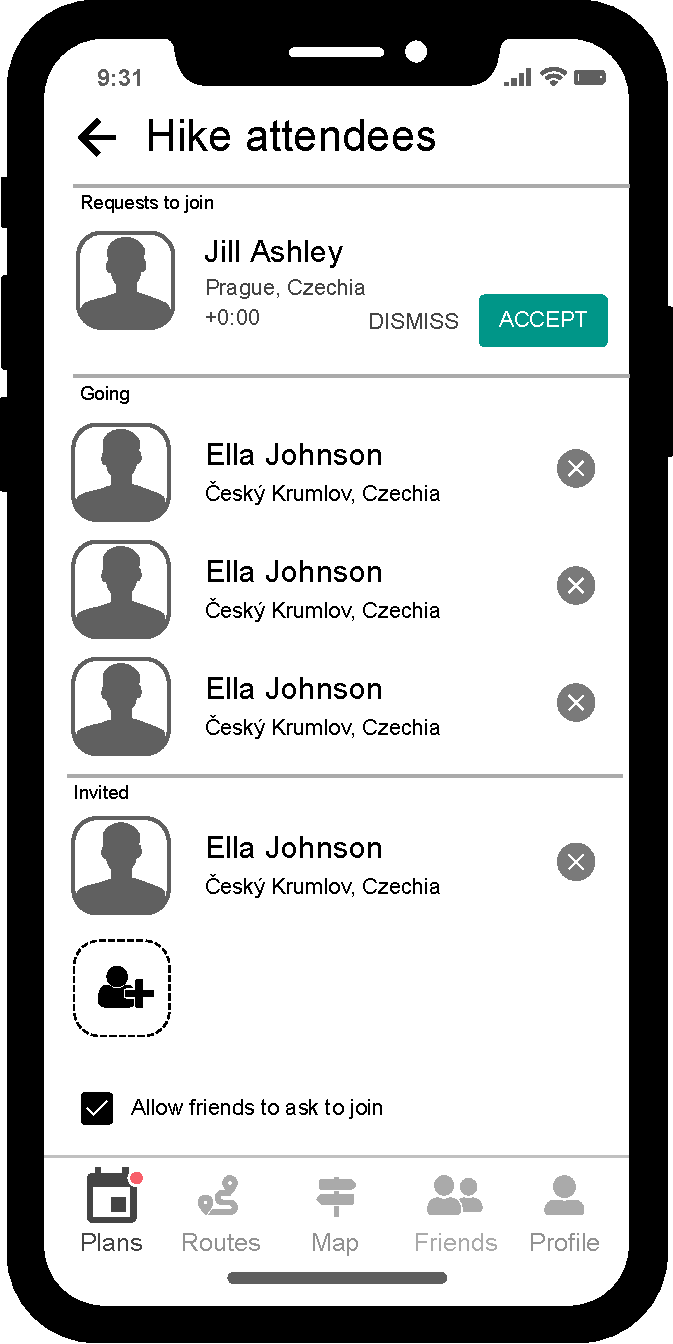
\includegraphics[width=0.3\textwidth]{Images/appScreens/plans-my-plans-detail-people.pdf}}\hfill
    \caption{My plans. Detail of a hike planned by the user, and a view of the invited and going people.}
    \label{fig:plan-my-plans}
\end{figure}

The `history' section~(fig.\ref{fig:plan-history}) of the `Plans' tab is the same as the `My plans' section, except all the hikes are in the past.
Each hikes' map contains the planned route, and the real route in case the user didn't precisely follow the plan.
This hike can be repeated by pressing the `Plan a hike' button and choosing whether to use the originally planned or the actually taken route.
Then the user is again taken to the planning UI.

\begin{figure}[h!]
    \centering
    \tmpframe{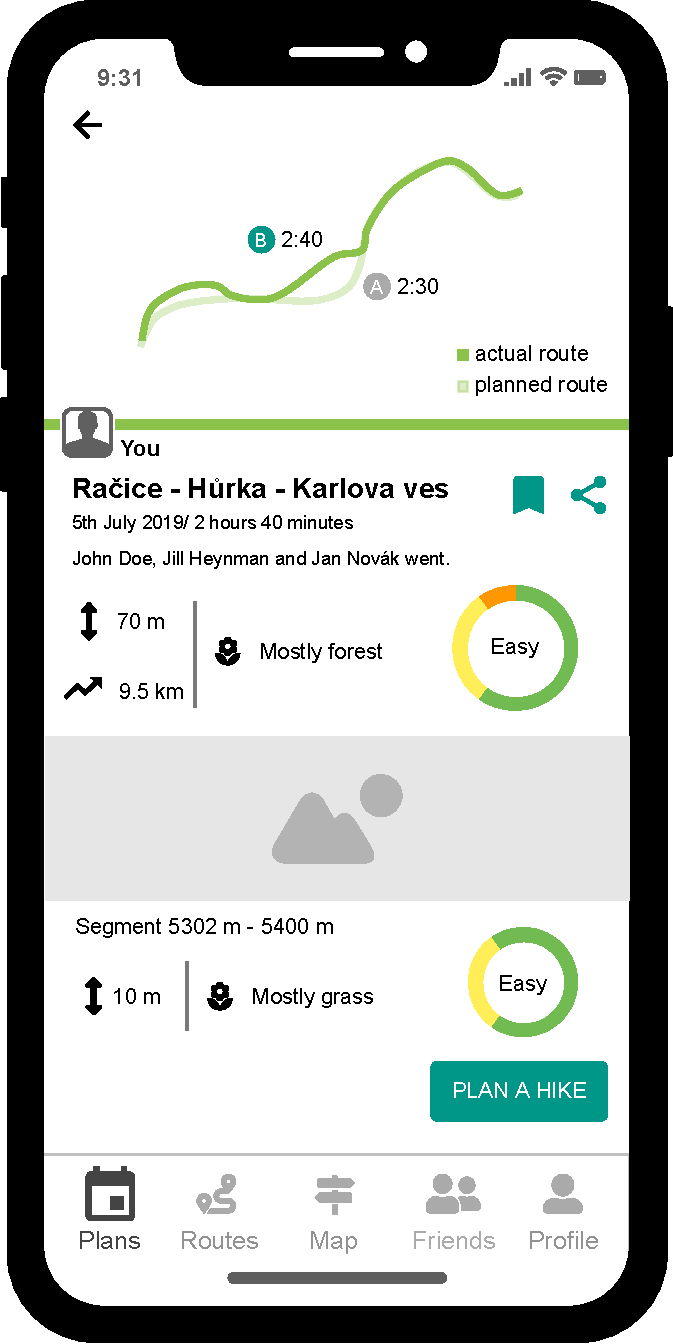
\includegraphics[width=0.4\textwidth]{Images/appScreens/plans-history-detail.pdf}}\hfill
    \caption{Detail of a historic hike.}
    \label{fig:plan-history}
\end{figure}

\section{Routes tab}
The `Routes' tab~(fig.\ref{fig:routes}) contains a filterable list of saved routes.
The only difference between a hike card and a route card is the fact that routes are not planned, so they don't include a host, people who are going, or the date they are planned for.

\begin{figure}[h!]
    \centering
    \tmpframe{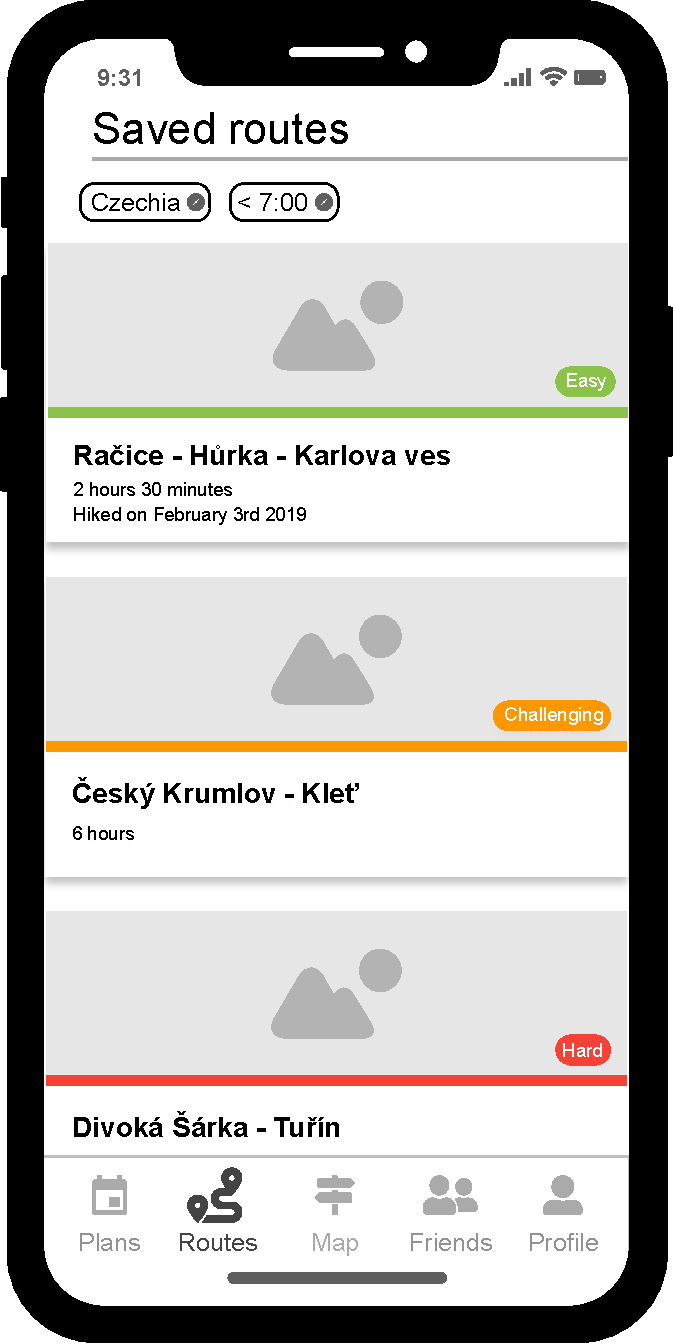
\includegraphics[width=0.4\textwidth]{Images/appScreens/routes.pdf}}\hfill
    \tmpframe{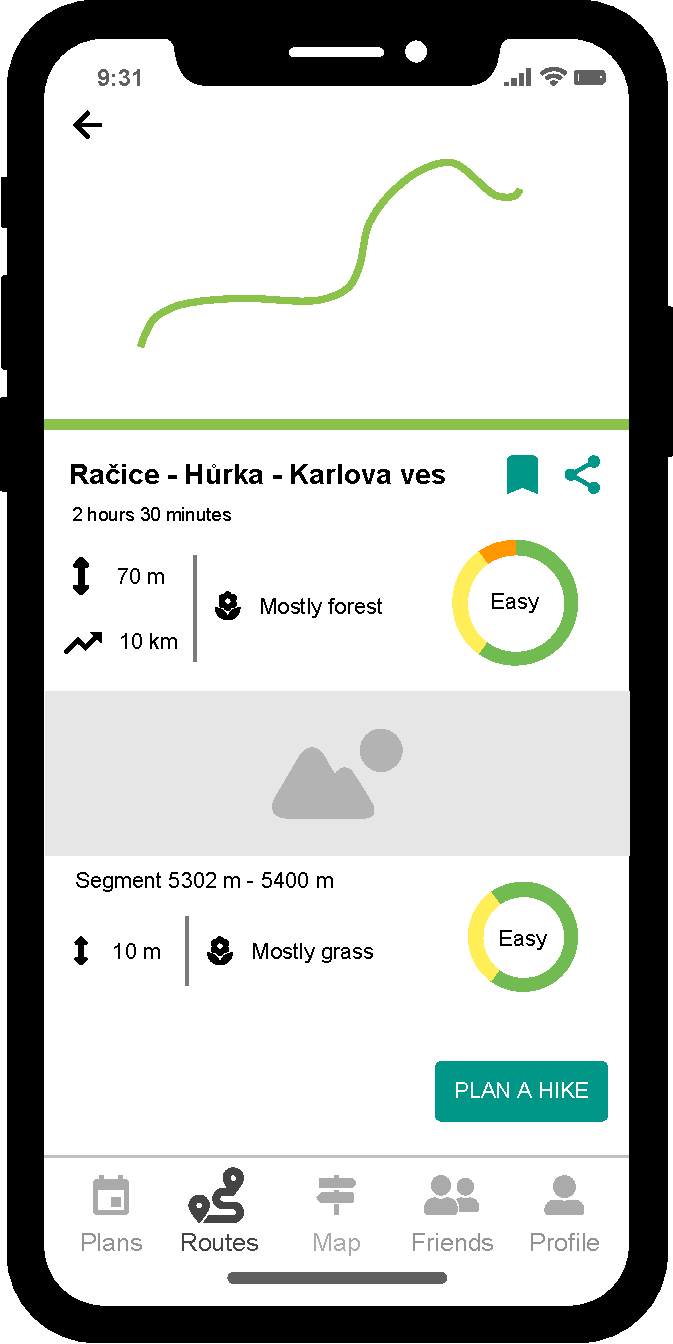
\includegraphics[width=0.4\textwidth]{Images/appScreens/routes-detail.pdf}}\hfill
    \caption{Routes tab. Detail of a route.}
    \label{fig:routes}
\end{figure}

\section{Friends tab}
Finally, the last tab is the `Friends' tab.
It contains a view of all the user's friends, as well as any pending friendship requests.
The detail of a user's profile is similar to the user who is signed in, but contains only basic information.
The profile is shareable, and the friend can also be removed from the user's friends list.
This is confirmed by a confirmation dialogue, warning the user about the fact that they will be removed from one another's plans.

\begin{figure}[h!]
    \centering
    \tmpframe{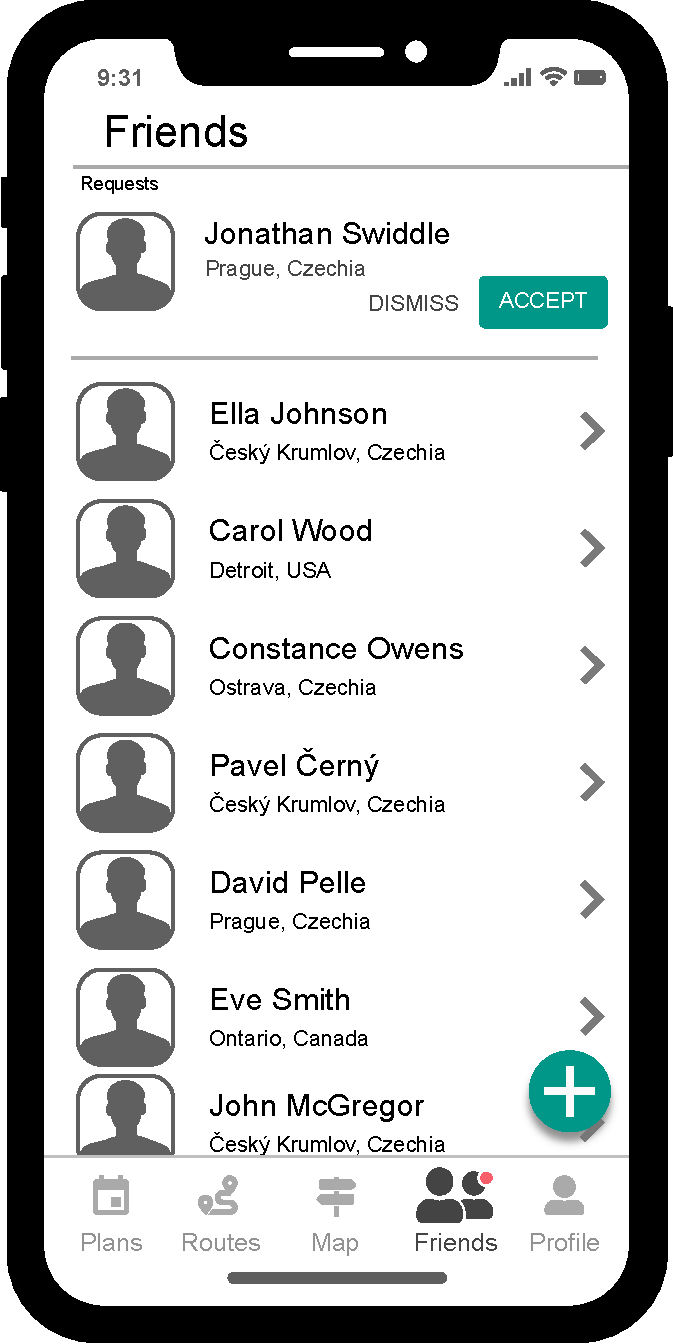
\includegraphics[width=0.3\textwidth]{Images/appScreens/friends.pdf}}\hfill
    \tmpframe{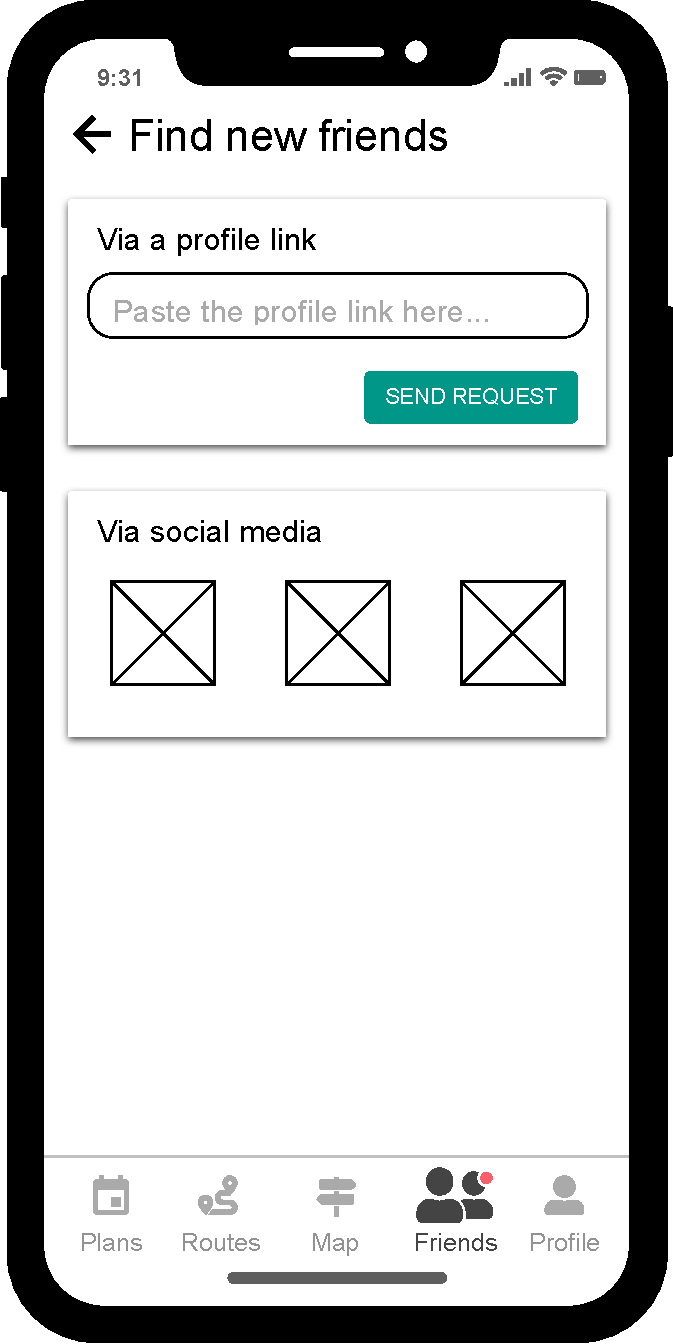
\includegraphics[width=0.3\textwidth]{Images/appScreens/friends-find.pdf}}\hfill
    \tmpframe{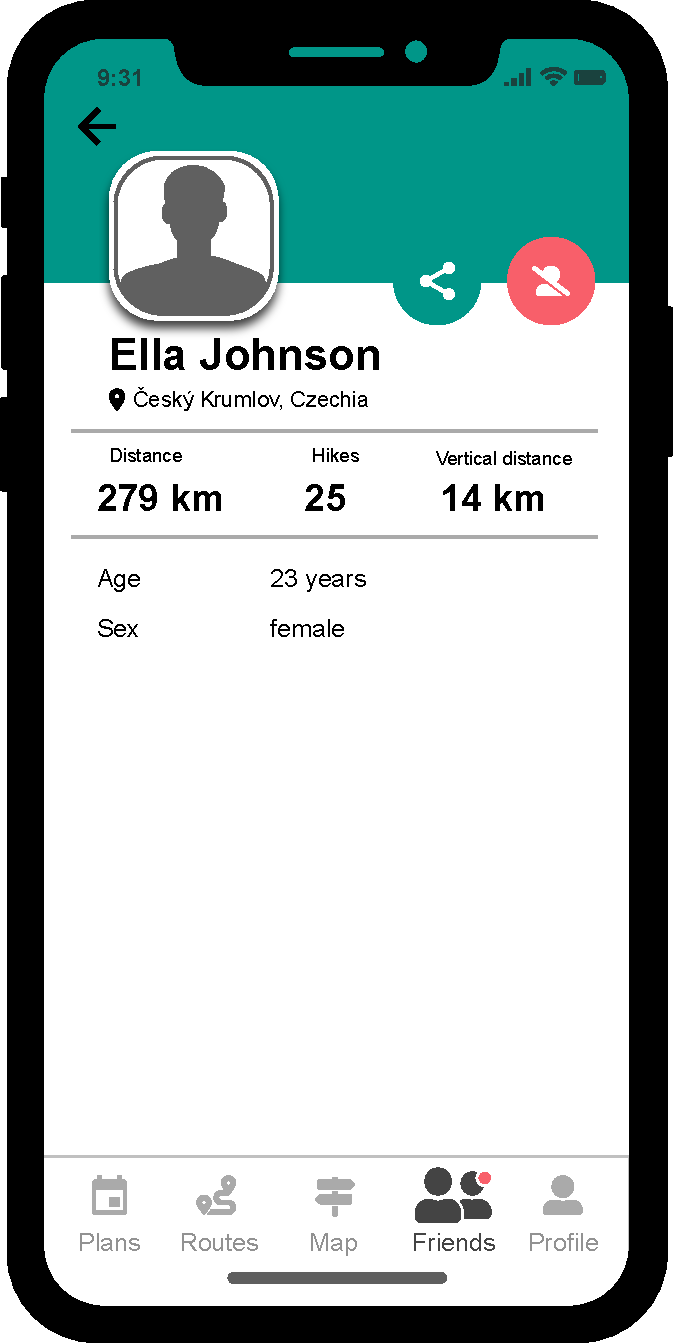
\includegraphics[width=0.3\textwidth]{Images/appScreens/friends-detail.pdf}}
    \caption{Friends tab, finding new friends and the user profile of a friend.}
    \label{fig:routes}
\end{figure}

\section{Navigation mode}
The application allows a user to navigate a planned route using a map and written directions (fig.\ref{fig:navigation}).
Once a hike is started, the view is switched to the `Map' tab.
The route is visualized on the map in colours of respective hiking trails and the user's position is highlighted.
There's also an overview of the difficulty of the current part of the route, and the user is notified if they are lagging behind the plan.
If the user wants to see something else than the navigation mode, they can use the close button on the top right, or just switch between tabs.
The navigation mode stays alive and accessible through a permanent notification.

\begin{figure}[h!]
    \centering
    \tmpframe{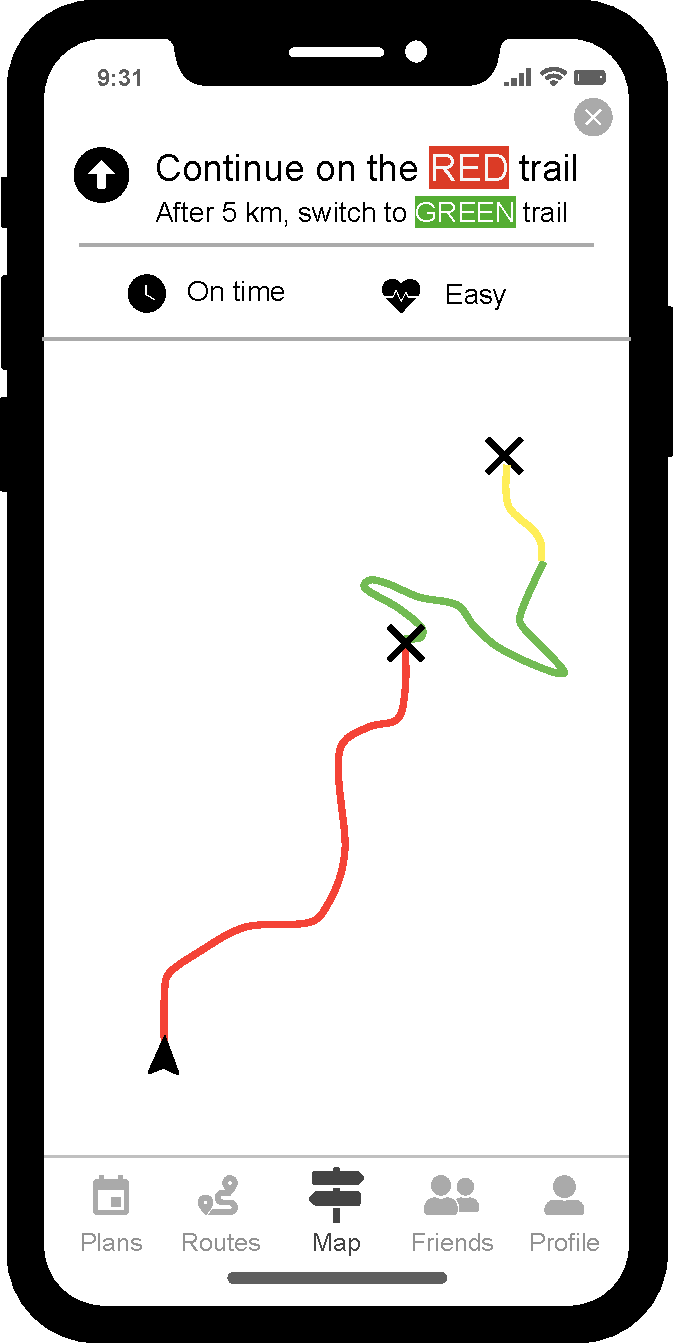
\includegraphics[width=0.4\textwidth]{Images/appScreens/navigation.pdf}}
    \label{fig:navigation}
\end{figure}
\chapter{Architecture}
\linebreak
In this chapter I aim to describe the proposed architecture of the solution, starting with a high-level glance -- the component diagram.

The smart wearable gadget will require an application to propagate the data from the heart rate sensor to the smart phone application.
Once the raw data is received, it is combined with GPS data and forwarded through the 'biometric and GPS raw data exchange' interface to the IoT platform, where it gets processed and saved.
When the smart phone application requires it, it requests the processed data through the 'processed data retrieval' and displays it.

\begin{figure}[h]
    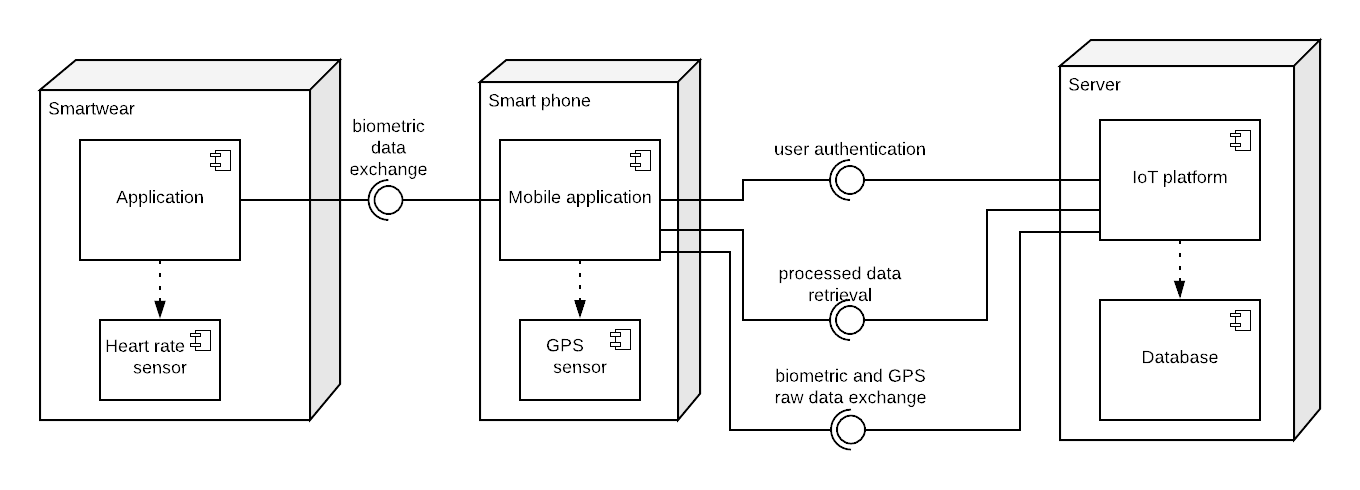
\includegraphics[width=\textwidth]{component.png}
    \caption{Component diagram of the designed IoT solution}
\end{figure}

\setsecnumdepth{part}
\chapter{Conclusion}
\linebreak
For now, I have been spending time mostly thinking about the importance of different features, evaluating the costs of having some compared to others, and how the use cases of existing apps apply to mine.
I have also thought out a high-level architectural model for communication between the components.

\bibliographystyle{iso690}
\bibliography{mybibliographyfile}

\setsecnumdepth{all}
\appendix

\chapter{Acronyms}
\begin{description}
	\item[IoT] Internet of Things -- \textit{The interconnection via the Internet of computing devices embedded in everyday objects, enabling them to send and receive data} \cite{IoT-dictionary} without requiring human-to-human or human-to-computer interaction. \cite{IoT-definition-no-interaction}
	\item[PoC] Proof of Concept -- \textit{Evidence, typically deriving from an experiment or pilot project, which demonstrates that a design concept, business proposal, etc. is feasible.} \cite{PoC-dictionary}
\end{description}


% \chapter{Contents of enclosed CD}

%change appropriately

% \begin{figure}
% 	\dirtree{%
% 		.1 readme.txt\DTcomment{the file with CD contents description}.
% 		.1 exe\DTcomment{the directory with executables}.
% 		.1 src\DTcomment{the directory of source codes}.
% 		.2 wbdcm\DTcomment{implementation sources}.
% 		.2 thesis\DTcomment{the directory of \LaTeX{} source codes of the thesis}.
% 		.1 text\DTcomment{the thesis text directory}.
% 		.2 thesis.pdf\DTcomment{the thesis text in PDF format}.
% 		.2 thesis.ps\DTcomment{the thesis text in PS format}.
% 	}
% \end{figure}

\end{document}
